% !TEX root = main.tex


% 文章的主体架构章节数均在此设计编辑。


\documentclass[UTF8,twoside,zihao=-4,AutoFakeBold,scheme=chinese,openany]{ctexbook}
\usepackage{graphicx}
\usepackage[ruled]{algorithm2e}
\usepackage[normalem]{ulem}
% 输入配置文件,例如调用的宏包(公式,插图等)

%设置文章格式

\usepackage[final]{pdfpages}

\usepackage{geometry}
\usepackage{makecell}
\usepackage{caption}
\usepackage{multirow}
\usepackage{booktabs}
\makeatletter
\let\c@lofdepth\relax
\let\c@lotdepth\relax
\makeatother
\usepackage{subfigure}
\usepackage{float}
\usepackage[titles,subfigure]{tocloft}
\usepackage{soul}
\usepackage{color,xcolor}
\usepackage{setspace}
\usepackage{titletoc}
\usepackage{longtable}
\usepackage[list=off]{bicaption}
\usepackage[hidelinks]{hyperref}
% \usepackage{mathptmx} %设置数学公式为新罗马字体
\usepackage{amsmath} %几个数学宏包
\usepackage{fontspec}
%\usepackage{caption2}


\AtBeginDocument{\DeclareMathAlphabet{\mathbf}{OT1}{cmr}{bx}{n}}







% 设置页边距
\geometry{a4paper,top=3cm,bottom=3cm,left=3cm,right=3cm}

% 设置行间距 1.5倍
%\linespread{1.4}\selectfont

% 设置段与段之间的垂直距离 \parskip默认橡皮长度是0pt plus 1pt
\setlength{\parskip}{0pt}
%\setlength{\baselineskip}{20pt}
% \setlength{\parindent}{0pt}

% 行间距={}*字体里面的第二个{},对于xiaosi而言就是1等于20磅
\linespread{1}\selectfont

%设置字体
% 设置英文字体
\setmainfont{Times New Roman}[
    BoldFont = Times New Roman Bold,
    ItalicFont = Times New Roman Italic,
    BoldItalicFont = Times New Roman Bold Italic
]

\setsansfont{Times New Roman}[
    BoldFont = Times New Roman Bold,
    ItalicFont = Times New Roman Italic,
    BoldItalicFont = Times New Roman Bold Italic
]

\setmonofont{Times New Roman}[
    BoldFont = Times New Roman Bold,
    ItalicFont = Times New Roman Italic,
    BoldItalicFont = Times New Roman Bold Italic
]

%设置字号,举例\xiaosi表示的是20磅行距,\xiaosid对应的是单倍行距


\usepackage{ctexsize,type1cm}
\newcommand{\chuhaod}{\fontsize{42pt}{54.6pt}\selectfont}
\newcommand{\xiaochud}{\fontsize{36pt}{46.8pt}\selectfont}
%\newcommand{\yihao}{\fontsize{26pt}{39pt}\selectfont}
%\newcommand{\xiaoyi}{\fontsize{24pt}{36pt}\selectfont}   
\newcommand{\erhaod}{\fontsize{22pt}{28.6pt}\selectfont}          
\newcommand{\xiaoerd}{\fontsize{18pt}{23.4pt}\selectfont}          
\newcommand{\sanhaod}{\fontsize{16pt}{20.8pt}\selectfont}        
\newcommand{\xiaosand}{\fontsize{15pt}{19.5pt}\selectfont}        
\newcommand{\sihaod}{\fontsize{14pt}{18.2pt}\selectfont}            
\newcommand{\xiaosid}{\fontsize{12pt}{15.6pt}\selectfont}            
%\newcommand{\wuhao}{\fontsize{10.5pt}{20pt}\selectfont}
%\newcommand{\xiaowu}{\fontsize{9pt}{13.5pt}\selectfont}    
%\newcommand{\liuhao}{\fontsize{7.5pt}{11.25pt}\selectfont}

\newcommand{\chuhao}{\fontsize{42pt}{42pt}\selectfont}
\newcommand{\xiaochu}{\fontsize{36pt}{36pt}\selectfont}
\newcommand{\yihao}{\fontsize{26pt}{39pt}\selectfont}
\newcommand{\xiaoyi}{\fontsize{24pt}{36pt}\selectfont}   
%\newcommand{\erhao}{\fontsize{22pt}{33pt}\selectfont}          
\newcommand{\xiaoer}{\fontsize{18pt}{27pt}\selectfont}          
\newcommand{\sanhao}{\fontsize{16pt}{20pt}\selectfont}        
\newcommand{\xiaosan}{\fontsize{15pt}{20pt}\selectfont}        
\newcommand{\sihao}{\fontsize{14pt}{20pt}\selectfont}            
\newcommand{\xiaosi}{\fontsize{12pt}{20pt}\selectfont}            
\newcommand{\wuhao}{\fontsize{10.5pt}{20pt}\selectfont}
\newcommand{\xiaowu}{\fontsize{9pt}{13.5pt}\selectfont}    
\newcommand{\liuhao}{\fontsize{7.5pt}{11.25pt}\selectfont}

%使用公式,表格,图片
\usepackage{mathtools,amsmath,amssymb,graphicx,array,float}

%按照章节编号
\numberwithin{figure}{chapter}
\numberwithin{table}{chapter}
\numberwithin{equation}{chapter}

%图、表、公式格式改为 X-X
\renewcommand\thefigure{\arabic{chapter}-\arabic{figure}}
\captionsetup[figure]{labelsep=space}

\renewcommand\thetable{\arabic{chapter}-\arabic{table}}
\captionsetup[table]{labelsep=space}

\renewcommand\theequation{\arabic{chapter}-\arabic{equation}}

%设置图表英文标题格式
\captionsetup{font={stretch=1.1}} %调整中英文图表标题的行距
\setlength{\abovecaptionskip}{6pt} %调整图表标题与图片和表格之间的距离
%\setlength{\belowcaptionskip}{1pt} 
\captionsetup[figure][bi-second]{name=\wuhao Fig.}
\captionsetup[table][bi-second]{name=\wuhao Table}




% 设置页眉面脚
%% 设置章节前的页码格式
%\usepackage[pagestyles]{titlesec}
%\newpagestyle{MyStyle}{
%  \setfoot{}{\Roman{page}}{}
%%  \headrule
%}

\usepackage{fancyhdr}

%\fancypagestyle{abstract}
%{
%	\fancyhf{}
%	\renewcommand{\headrulewidth}{0.5pt}
%	%	\renewcommand{\footrulewidth}{0mm}
%	\fancyfoot[C]{\songti\xiaowu \Roman{page}}
%	\fancyhead[C]{\wuhao \leftmark}
%}

%重新设置plain,chapter设置页眉时会调用plain,因此需要重新定义plain,不能设置为其他名称



\fancypagestyle{plain}{
	\fancyhf{}
	\fancyfoot[C]{\songti\xiaowu  \Roman{page} }
	\fancyhead[C]{\songti\wuhao \leftmark}
}





%页眉设置,博士和硕士学位论文请在下面自行修改
\fancypagestyle{body}{
    \fancyhf{}
    \fancyfoot[C]{\songti\xiaowu \thepage}
    \fancyhead[CO]{\songti\wuhao \rightmark}
    \fancyhead[CE]{\songti\wuhao 重庆邮电大学硕士学位论文}
}

\fancypagestyle{others}{
	\fancyhf{}
	\fancyfoot[C]{\songti\xiaowu \thepage}
	\fancyhead[CO]{\songti\wuhao \leftmark}
	\fancyhead[CE]{\songti\wuhao 重庆邮电大学硕士学位论文}
}







%设置双线页眉
%\makeatletter
%\def\headrule{
%    {\if@fancyplain\let\headrulewidth\plainheadrulewidth\fi%
%    \hrule\@height 1.0pt \@width\headwidth\vskip1pt%上面线为1pt粗
%    \hrule\@height 0pt \@width\headwidth  %下面0.5pt粗
%    \vskip-2\headrulewidth\vskip-1.2pt}    %两条线的距离1pt
%    \vspace{6mm}}     %双线与下面正文之间的垂直间距
%\makeatother

%设置双线页脚
\makeatletter
\def\footrule{
    {\if@fancyplain\let\footrulewidth\plainfootrulewidth\fi%
    \hrule\@height 0pt \@width\headwidth          %上面0.5pt粗
    \vskip 1pt
    \hrule\@height 0pt \@width\headwidth %下面线为1pt粗
    \vskip-2\headrulewidth\vskip-1.2pt}    %两条线的距离1pt
    \vspace{8mm}}     %双线与下面正文之间的垂直间距
\makeatother

%\renewcommand\thechapter{\arabic{chapter}}

%设置文章格式
\ctexset {
    contentsname={目 \quad 录},
    listfigurename={图目录},
    listtablename={表目录},
    figurename={\wuhao 图},
    tablename={\wuhao 表},
    bibname={参考文献},
    appendixname={附录},
    chapter={
    	name={第,章},
    	aftername=\enspace,
    	number={\arabic{chapter}},
        beforeskip={-2pt},
        afterskip={18pt},
        nameformat={\heiti\sanhao\centering\mdseries}, 
        titleformat={\heiti\sanhao\centering\mdseries},
    },
    section={
    	aftername=\enspace,
    	beforeskip={18pt},
    	afterskip={6pt},
        format={\heiti\sihao\leftline},
    },
    subsection={
    	aftername=\enspace,
    	beforeskip={12pt},
    	afterskip={6pt},
        format={\heiti\sihao\leftline},
    },
    subsubsection={
    	aftername=\enspace,
    	beforeskip={12pt},
    	afterskip={6pt},
        format={\heiti\xiaosi\leftline},
    }
}



% 目录中的章加点
%\usepackage[titles]{tocloft}
%\renewcommand{\cftdot}{$\cdot$}
%\renewcommand{\cftdotsep}{1.5}
%\setlength{\cftbeforechapskip}{10pt}
%
%\renewcommand{\cftchapleader}{\cftdotfill{\cftchapdotsep}}
%\renewcommand{\cftchapdotsep}{\cftdotsep}
%\makeatletter
%\renewcommand{\numberline}[1]{
%\settowidth\@tempdimb{#1\hspace{0.5em}}
%\ifdim\@tempdima<\@tempdimb
%  \@tempdima=\@tempdimb
%\fi
%\hb@xt@\@tempdima{\@cftbsnum #1\@cftasnum\hfil}\@cftasnumb}
%\makeatother

% 设置目录字体尺寸
%\renewcommand{\cftchapfont}{\heiti\xiaosi}
%\renewcommand{\cftsecfont}{\heiti\xiaosi}
%\renewcommand{\cftsubsecfont}{\songti\xiaosi}
%\renewcommand{\cftsubsubsecfont}{\songti\xiaosi}

% 设置目录标题深度
\setcounter{secnumdepth}{3}
\setcounter{tocdepth}{2}


% 设置目录标题缩进,字体等
\titlecontents{chapter}[3.8em]{\heiti\xiaosi}{\contentslabel{3.8em}}{\hspace{-3.76em}}{\titlerule*[0.4pc]{$\cdot$}\contentspage\hspace*{0.01em}}
\titlecontents{section}[3.8em]{\songti\xiaosi}{\contentslabel{2em}}{\hspace{-2em}}{\titlerule*[0.4pc]{$\cdot$}\contentspage\hspace*{0.01em}}
\titlecontents{subsection}[6.5em]{\songti\xiaosi}{\contentslabel{2.7em}}{\hspace{-2.7em}}{\titlerule*[0.4pc]{$\cdot$}\contentspage\hspace*{0.01em}}

%设置图表目录标题格式
\titlecontents{figure}[0pt]{\songti\xiaosi\settowidth{\hangindent}{图~\thecontentslabel\ \ }}{图~\thecontentslabel\ \ }{}{\hspace{.25em}\titlerule*[4pt]{$\cdot$}\contentspage}


\titlecontents{table}[0pt]{\songti\xiaosi\settowidth{\hangindent}{表~\thecontentslabel\ \ }}{表~\thecontentslabel\ \ }{}{\hspace{.25em}\titlerule*[4pt]{$\cdot$}\contentspage}

%\dottedcontents{subsubsection}[4cm]{\normalsize}{4em}{4pt}

%使用代码排版包
\usepackage{listings}
\usepackage{color}
\lstset{%
    frame=shadowbox,
    extendedchars=false,            % 不使用xelatex而使用CJK方式处理汉字
    language=python,
    basicstyle=\sffamily,           % 设置整体格式
    keywordstyle=\bfseries,         % 关键字格式
    commentstyle=\rmfamily\itshape, % 注释格式
    stringstyle=\ttfamily,          % 字符串格式
    columns=flexible,
    escapechar=',                   % 注释中显示汉字,eg //'一个整数'
    tabsize=4,
    numbers=left,
    numberstyle=\small,             % 行号字体设置
    stepnumber=1,                   % 行号距离设置,1代表每行加行号
    numbersep=8pt,                  % 行号和代码距离设置
    backgroundcolor=\color{white},
    showspaces=false,               % show spaces adding particular underscores
    showstringspaces=false,         % 使用下划线连接字符串
    showtabs=false,
    frame=single,                   % 给代码加边框
    captionpos=b,                   % sets the caption-position to bottom
    breaklines=true,                % 自动换行设置
    breakatwhitespace=false,        % sets if automatic breaks should only happen at whitespace
    escapeinside={\%*}{*)},         % if you want to add a comment within your code
    xleftmargin=2em,                % 设置左边距,宽度默认是与页芯等宽的
    xrightmargin=2em,               % 设置右边距,宽度默认是与页芯等宽的
    aboveskip=1em                   % 设置上边距
}

%设置自定义变量
\newcommand\degree{^\cire}

% 定义文献引用格式,\cite正常引用 \supercite右上角引用
\usepackage{cite}
\newcommand{\upcite}[1]{\textsuperscript{\textsuperscript{\cite{#1}}}}
\newcommand\supercite[2][]{%
\textsuperscript{\cite[#1]{#2}}
}

\usepackage{enumitem}
\setlist[description]{
    itemsep=-5pt,
    font=\songti,
}

% 定义中文封面环境
\newenvironment{titletabbing}
{\par\bfseries\songti\sihao\tabbing}
{\endtabbing\par}

\usepackage[nottoc]{tocbibind}
\endinput



%取消章节编号
\makeatletter
\newcommand\specialsectioning{
	\setcounter{secnumdepth}{-2}
}
\makeatother




\begin{document}
	
% 封面页及扉页
\pagestyle{empty}
% !TEX root = main.tex
\quad
% 封面及扉页
\vspace{-3mm}

\begin{center}

%\begin{spacing}{1.0}


\erhaod 重\hspace{11pt}庆\hspace{11pt}邮\hspace{11pt}电\hspace{11pt}大\hspace{11pt}学\\[1mm]
\xiaosid CHONGQING UNIVERSITY OF POSTS AND TELECOMMUNICATIONS\\
\vspace{14mm}

%根据学位论文种类自行编辑中英文名称,硕士、工程硕士名称请参照写作指南
% \chuhaod 博士学位论文\\[2mm]
% \sanhaod DOCTORAL DISSERTATION

\chuhaod 硕士学位论文\\
\sanhaod MASTER THESIS

%\chuhaod 专业学位硕士学位论文\\
%\sanhaod MASTER THESIS FOR PROFESSIONAL DEGREE

%\end{spacing}

\vspace{13mm}

        
        \begin{figure*}[h]
        	\centering
        	
\includegraphics[scale=0.475]{chapters/logo2.jpg}
        \end{figure*}
\end{center}

\vspace{3mm}

		\begin{table}[h]

		\renewcommand\arraystretch{2}
		\begin{tabular}{p{3cm}p{10cm}}
			
%输入论文题目如果过长可以在第二行进行输入,如果不需要第二行请自行删除,注意字体里面的\xiaoerd表示的是单倍行距,在封面页各种字体后面都加一个d

			\makecell[c]{\songti\bfseries\xiaoerd 论文题目}	& \makecell[c]{\songti\bfseries\xiaoerd 基于显著锚点几何嵌入的点云配准} \\ 
			\cline{2-2}
			 	&  \makecell[c]{\songti\bfseries\xiaoerd 方法研究}\\ 
			\cline{2-2}
			\end{tabular}
	\end{table}

\vspace{5mm}

\begin{table}[!hb]
			\centering
	\renewcommand\arraystretch{2}
	
%这是一个表格,请在相应位置输入相关信息 
       \begin{tabular}{p{2.5cm}p{9.4cm}}		
		\makecell[c]{\songti\bfseries\sanhaod 学科专业} 	& \makecell[c]{\songti\bfseries\sanhaod 电子信息} \\
		\cline{2-2} 
		\makecell[c]{\songti\bfseries\sanhaod 学\qquad 号} 	&  \makecell[c]{\songti\bfseries\sanhaod } \\
		\cline{2-2} 
		\makecell[c]{\songti\bfseries\sanhaod 作者姓名} 	& \makecell[c]{\songti\bfseries\sanhaod } \\
		\cline{2-2} 
		\makecell[c]{\songti\bfseries\sanhaod 指导教师} 	& \makecell[c]{\songti\bfseries\sanhaod } \\
		\cline{2-2} 
		\makecell[c]{\songti\bfseries\sanhaod 学\qquad 院} 	&  \makecell[c]{\songti\bfseries\sanhaod } \\
		\cline{2-2}
	
			
			
%如果是专硕,需要改为专业学位类别,表格列宽需要调整,请将上述部分替换为下面所示
%	\begin{tabular}{p{3.5cm}p{8.1cm}}
%	\makecell[c]{\songti\bfseries\sanhaod 专业学位类别} 	& \makecell[c]{\songti\bfseries\sanhaod XXXX} \\
%	\cline{2-2} 
%	\makecell[c]{\songti\bfseries\sanhaod 学\qquad \qquad 号} 	&  \makecell[c]{\songti\bfseries\sanhaod XXXX} \\
%	\cline{2-2} 
%	\makecell[c]{\songti\bfseries\sanhaod 作 \enspace 者\enspace 姓 \enspace 名} 	& \makecell[c]{\songti\bfseries\sanhaod XXXX} \\
%	\cline{2-2} 
%	\makecell[c]{\songti\bfseries\sanhaod 指 \enspace 导\enspace 教 \enspace 师} 	& \makecell[c]{\songti\bfseries\sanhaod XXXX} \\
%	\cline{2-2} 
%	\makecell[c]{\songti\bfseries\sanhaod 学\qquad \qquad 院} 	& \makecell[c]{\songti\bfseries\sanhaod XXXX}  \\
%	\cline{2-2}	
 		
		\end{tabular}
	\end{table}

\clearpage


\begin{table}[ht]
	\centering
	\renewcommand\arraystretch{1.5}
	\begin{tabular}{p{2cm}p{4.5cm}p{1.5cm}p{4cm}}
		
%这也是一个表格,请在相关位置输入相关信息		
		\makecell[l]{\songti\xiaosid 学校代码} 	&	\makecell[c]{\xiaosid 10617} &	\makecell[c]{\xiaosid UDC} & \makecell[c]{\xiaosid 004.93} \\
		\cline{2-2} \cline{4-4}
		
		\makecell[l]{\songti\xiaosid 分\hspace{6pt}类\hspace{6pt}号} 	&\makecell[c]{\xiaosid TP391.4} &\makecell[c]{\songti\xiaosid 密级} & \makecell[c]{\xiaosid 公开} \\
		\cline{2-2} \cline{4-4}
	   
	\end{tabular}
\end{table}

		\vspace{1mm}

\begin{center}

	


		\songti\xiaochud\textbf{学\hspace{36pt}位\hspace{36pt}论\hspace{36pt}文}\\
		
		\vspace{15mm}


\makeatletter
\newcommand\dlmu[2][4cm]{\hskip1pt\underline{\hb@xt@ #1{\hss#2\hss}}\hskip1pt}
\makeatother
%请在此输入论文题目,如果一行不够请自行添加
\dlmu[14cm]{\songti\bfseries\xiaoerd 基于显著锚点几何嵌入的点云配准方法研究}\\
\vspace{5mm}
%请在此输入作者姓名
\dlmu[5cm]{\songti\bfseries\sanhaod  \quad }\\


\end{center}

\vspace{10mm}

	\begin{table}[h]
	\renewcommand\arraystretch{2}
	\begin{tabular}{p{3cm}p{9cm}}
%请在相关位置输入指导教师姓名,如果有第二导师请在第二行输入,如果没有,可以自行删去第二行
		\makecell[r]{\songti\xiaosid 指导教师}	& \makecell[c]{\songti\bfseries\sanhaod  \quad \,  \quad \, \qquad \hspace{16pt}} \\
		\cline{2-2}
		&  \makecell[c]{\songti\bfseries\sanhaod \quad \,  \quad \, \qquad \hspace{16pt}}\\ 
		\cline{2-2}
	\end{tabular}
\end{table}

\vspace{30mm}


	\begin{table}[!hb]
	\centering
	\renewcommand\arraystretch{2}
	\begin{tabular}{p{2.6cm}p{0.4cm}p{0.8cm}p{2.8cm}p{2.6cm}p{4cm}}
%请在相关位置输入相关信息,工程硕士、学硕及博士的部分类容有不同,请自行修改	
		\makecell[l]{\songti\xiaosid 申请学位级别} 	&	\multicolumn{3}{c}{\songti\bfseries\sihaod 硕士} &	\makecell[c]{\songti\xiaosid 学科专业} & \makecell[c]{\songti\bfseries\sihaod 电子信息}\\
	\cline{2-4} \cline{6-6}
	
	% \makecell[l]{\songti\xiaosid 专业学位领域} 	& \multicolumn{5}{c}{\songti\bfseries\sihaod XXXXXX} \\
	%  \cline{2-6}
	 
	 \multicolumn{2}{l}{\songti\xiaosid 答辩委员会主席} 	&	\multicolumn{2}{c}{\songti\bfseries\sihaod   \quad  } &	\makecell[c]{\songti\xiaosid 论文答辩日期} & \makecell[c]{\songti\bfseries\sihaod 2023年5月20日}\\
	 \cline{3-4} \cline{6-6}
	 
	 \multicolumn{3}{l}{\songti\xiaosid 学位授予单位和日期} & \multicolumn{3}{c}{\songti\bfseries\sihaod 重庆邮电大学 \qquad 2023年6月}\\
	 \cline{4-6}
	 

	 
	 	\end{tabular}
 \end{table}

\clearpage

\quad

\begin{center}
	
%	\begin{spacing}{1.0}
%英文论文题目自行修改
	\xiaoerd\textbf{Research on Point Cloud Registration Method Based on Geometric Embedding of Significant Anchor Points}\\
	
	\vspace{60mm}
%根据硕士或者博士,自行修改下面语句中的论文种类,标准请参照写作指南	
	% \xiaosand A Doctoral Dissertation Submitted to \\
	% Chongqing University of Posts and Telecommunications\\
	
		\xiaosan A Master Thesis Submitted to \\
	School of Chongqing University of Posts and Telecommunications\\
	
	
%	\end{spacing}

\vspace{60mm}

\begin{table}[!hb]
	\centering
	\renewcommand\arraystretch{2}
	\begin{tabular}{p{2.5cm}p{11cm}}
		
%这是一个表格,在相应位置输入相关信息		
		\makecell[r]{\sanhaod Discipline} 	& \makecell[c]{\bfseries\sanhaod Electronic and Information Engineering} \\
		\cline{2-2} 
		\makecell[r]{\sanhaod Student ID} 	&  \makecell[c]{\bfseries\sanhaod } \\
		\cline{2-2} 
		\makecell[r]{\sanhaod Author} 	& \makecell[c]{\bfseries\sanhaod } \\
		\cline{2-2} 
		\makecell[r]{\sanhaod Supervisor} 	& \makecell[c]{\bfseries\sanhaod } \\
		\cline{2-2} 
		\makecell[r]{\sanhaod School} 	&  \makecell[c]{\bfseries\sanhaod } \\
		\cline{2-2}			
	\end{tabular}
\end{table}



\end{center}
\clearpage







	 
	 	
	




	












% 原创性声明
% 原创性声明
%这一页无需改动,打印出来手动签名

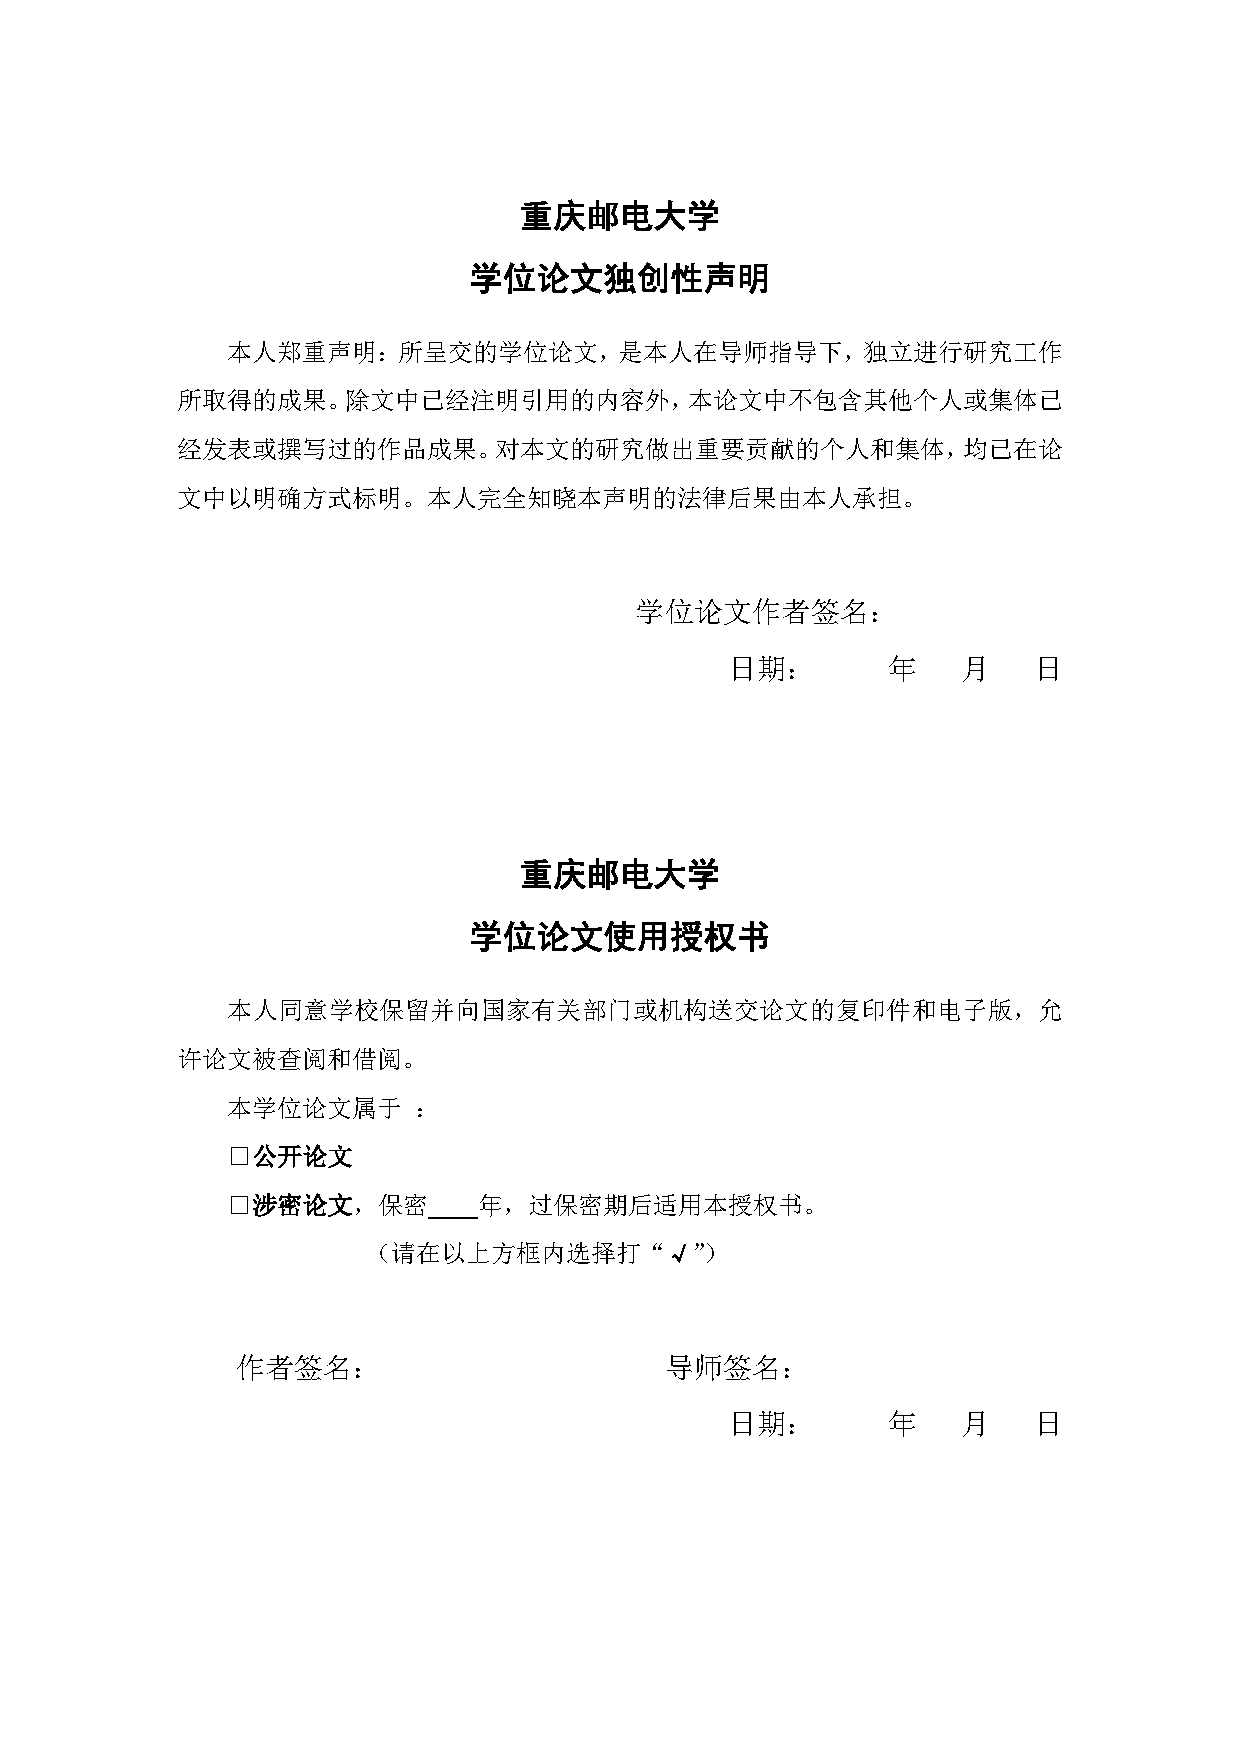
\includepdf{original.pdf}
\clearpage


\clearpage

%前序部分(中英文摘要,目录等,chapter后面不编号)
\frontmatter

%开始以大写罗马字母计页码
\pagenumbering{Roman}

\pagestyle{plain}
%页面格式
%\pagestyle{plain}

% 中文摘要页
%中文摘要,自行编辑内容



\chapter{摘 \quad 要}
\xiaosi
点云是一种用于表示三维空间中的对象的数据结构。它由许多离散的点组成,可以通过激光扫描仪、三维相机或其他传感器来捕捉和记录。由于这些传感器的视野有限,因此需要将多个点云合并成一个更大的点云,或将点云与先前的点云模型对齐以进行比较或更新,这个过程就是点云配准。点云配准是计算机视觉和机器人视觉中的重要问题,它们可以用于许多应用,例如三维建模、机器人导航、虚拟现实和医学影像分析。早期的点云配准主要集中于计算机合成数据集,然而随着社会的发展,越来越多的研究开始关注真实场景下的点云配准。但真实场景中普遍存在图案重复、几何形状较弱的困难区域,这些困难区域往往会由于特征相似导致点匹配的错误,影响变换矩阵的估计结果。

为了解决该问题,本文提出了一种基于显著锚点几何嵌入的点云配准方法。该方法嵌入显著锚点与超点之间的几何结构,以增强点特征的差异性和区分度。即使在源点云和目标点云中存在大量图案重复和弱几何区域,也能分辨出相似非重叠区域找到正确的点匹配。具体来说,首先通过锚点定位模块,在源点云和目标点云中定位识别能力最强、几何信息最丰富的超点对应作为显著锚点对应。采用非最大抑制算法,保证选定的一组显著锚点在点云中稀疏分布并且具有一定的几何结构。针对显著锚点,提出了一种基于锚点距离和角度的选择性几何结构嵌入算法,用于超点特征增强。这种显著锚点与超点之间的几何一致性,可以提高几何挑战性区域的特征区分度。然后,迭代更新以增强特征和锚点位置,获得最有效的显著锚点和超点特征。最后,通过在超点对应区域内寻找最近的相邻点来实现精确的点对应。

另外,本文提出了一种基于多模态融合的锚点定位点云配准方法,该方法通过将点云的结构特征和图像的纹理特征融合以提高几何挑战性区域的特征差异性。首先本文利用对齐模块将点云和图像数据对齐以找到超点与像素之间的对应关系。然后,利用融合模块将超点与对应像素之间的特征进行融合。该融合模块将点云特征和图像特征分别投影至模态无关和模态相关的两个子空间中,并先后在两个子空间中融合两种模态特征以达到减小域差异影响和防止信息丢失的作用。\\

% 学位论文是研究生从事科研工作的成果的主要表现,集中表明了作者在研究工作中获得的新发明、新理论或新见解,是研究生申请硕士或博士学位的重要依据,也是科研领域中的重要文献资料和社会的宝贵财富。
% 为进一步规范我校研究生学位论文撰写格式,提高研究生学位论文质量,参照国家标准《学位论文编写规则》(GB/T 7713.1-2006),结合我校实际,制定本模板。
\noindent\songti\textbf{关键词:} 点云配准,几何嵌入,弱几何区域,重复图案,多模态融合

\clearpage


% 英文摘要页
%英文摘要,自行编辑内容




\chapter{ABSTRACT}
\xiaosi
A point cloud is a data structure used to represent objects in three-dimensional space. It consists of many discrete points that can be captured and recorded by laser scanners, 3D cameras, or other sensors. Due to the limited field of view of these sensors, multiple point clouds need to be merged into a larger point cloud, or point clouds are aligned with previous point cloud models for comparison or updating. This process is point cloud registration. Point cloud registration is an important problem in computer vision and robot vision, and it can be used in many applications, such as 3D modeling, robot navigation, virtual reality, and medical image analysis. Early point cloud registration mainly focused on computer-synthesized datasets. However, with the development of society, more and more researchers began to focus on point cloud registration in real scenes. However, the geometrically challenging areas with repetitive patterns and low geometry commonly exist in real scenes, causing failure in point matching followed by inaccurate point cloud registration. 

In this thesis, this thesis propose a robust point cloud registration approach that embeds the geometry of salient anchors to enhance the discriminative ability of the point features even in the presence of a large number of repetitive patterns and low-geometry areas in the source and target point clouds. Specifically, an anchor location module is designed to locate corresponding superpoints with the most discriminative and the richest geometric information as salient anchors in the source and target. Non-maximum suppression is adopted to ensure the salient anchors are structure-preserved and sparsely distributed. With salient anchors, a selectively geometric structure embedding of anchorsuperpoint distances and angles is proposed for superpoint feature enhancement. This integration of geometry consistency between the salient anchors and superpoints can improve the distinction of features in those geometrically challenging areas. Afterwards, the enhanced features and anchor positions are updated in an iterative manner to acquire the most effective salient anchors and descriptive superpoint features. The updated features allow for accurate superpoint matches. Finally, accurate point correspondences are achieved by finding the nearest neighbour points within superpoints. 

In addition, this thesis proposes a point cloud registration method based on multimodal fusion for anchor location, which improves the feature diversity of geometrically challenging regions by fusing the structural features of the point cloud and the texture features of the image. First, this paper uses the alignment module to align the point cloud and image data to find the correspondence between superpoints and pixels. Then, a fusion module is used to fuse the features between the superpoints and the corresponding pixels. The fusion module projects the point cloud features and image features into two subspaces that are modality-independent and modality-dependent, and fuses the two modality features successively in the two subspaces to reduce the impact of domain differences and prevent information loss role.\\
% Dissertation /Thesis is postgraduate’s main academic performance to display her/his works of scientific research, which shows the author’s new invention, new theory or new opinion in her/his research. It is the crucial document for the graduate students to apply for degree, and it is also the important scientific research literature and the valuable wealth of society.

% In order to further standardize the format of dissertation/thesis writing and improve graduate dissertation/thesis quality, this temolate is formulated with reference to the national standard "Rules for Dissertation Writing" (GB/T 7713.1-2006) and the reality of CQUPT.
\noindent\textbf{Keywords:} Point cloud registration, Geometry embedding, Low-geometry area, Repetitive patterns, Multimodal fusion

\clearpage


% 目录
%\begin{spacing}{1.14}
\tableofcontents


\begingroup
\renewcommand*{\addvspace}[1]{}
%图目录
%\newcommand{\loflabel}{图}
%\renewcommand{\numberline}[1]{\loflabel~#1\hspace*{1em}}
\listoffigures

%表目录
%\newcommand{\lotlabel}{表}
%\renewcommand{\numberline}[1]{\lotlabel~#1\hspace*{1em}}
\listoftables
\endgroup

%\end{spacing}


%主要符号表
% 

\chapter{主要符号表}



\begin{table}[h]
	\renewcommand{\arraystretch}{1.5}
	\centering
	\begin{tabular}{p{2cm}p{10cm}p{1.5cm}}
		\toprule[1.5pt]
		\makecell[l]{\songti\xiaosi\bfseries 符号}&\makecell[l]{\songti\xiaosi\bfseries 说明}&\makecell[c]{\songti\xiaosi\bfseries 页码}\\
		\hline
		\makecell[l]{\wuhao c}&\makecell[l]{\wuhao 电磁波的相平面速度}&\makecell[c]{\wuhao 10}\\
		\bottomrule[1.5pt]
	\end{tabular}
     
\end{table}

\clearpage

%缩略词表
% 



\chapter{缩略词表}

\begin{table}[h]
	\renewcommand{\arraystretch}{1.5}
	\centering
	\begin{tabular}{p{2cm}p{8.5cm}p{3cm}}
		\toprule[1.5pt]
		\makecell[l]{\songti\xiaosi\bfseries 英文缩写}&\makecell[l]{\songti\xiaosi\bfseries 英文全称}&\makecell[l]{\songti\xiaosi\bfseries 中文全称}\\
		\hline
		\makecell[l]{\wuhao CQUPT}&\makecell[l]{\wuhao Chongqing University of Posts Telecommunications}&\makecell[l]{\wuhao 重庆邮电大学}\\
		\bottomrule[1.5pt]
	\end{tabular}
	
\end{table}

\clearpage

\clearpage

%% 开始章节写作,chapter后面开始编号,显示特定页眉页脚
\mainmatter
\pagenumbering{arabic}

%正文页眉避免英文全部大写
\renewcommand\thechapter{\arabic{chapter}}
\renewcommand{\chaptermark}[1]{\markboth{第 \thechapter 章 \ #1}{}}

% 第1章
\chapter{绪论}
\thispagestyle{others}
\pagestyle{others}
\xiaosi

\section{研究背景及意义}
近些年来,计算机视觉的发展让我们的生活越来越便利。与此同时,随着我国信息化水平和自动化进程的不断提高与推进,国家对计算机视觉的应用和发展也提出了更高要求。相比于二维图像,三维点云数据能更加清晰的表示我们所处的三维世界。图\ref*{fig:1-1}显示了两对激光雷达点云和图像的例子,它们分别取自于不同时间的同一场景。可以清晰的观察到,点云的几何结构在光照和季节变化的情况下能够保持基本不变,而图像的变化使得人眼也难以分辨出这对图像来自于同一场景。由于点云数据具有光照不变性,能够有效避免图像处理过程中的问题,因此越来越多的研究人员开始研究点云并从中获益。但是三维视觉传感器的视野范围是有限的,因此为了感知全局的环境,在应用中经常需要将若干不同位置采集的点云数据对齐到世界坐标系下。因此,点云配准已成为许多任务的基础问题,近年来备受关注。

\vspace{-0.1cm}
\begin{figure}[h]
    \centering 
    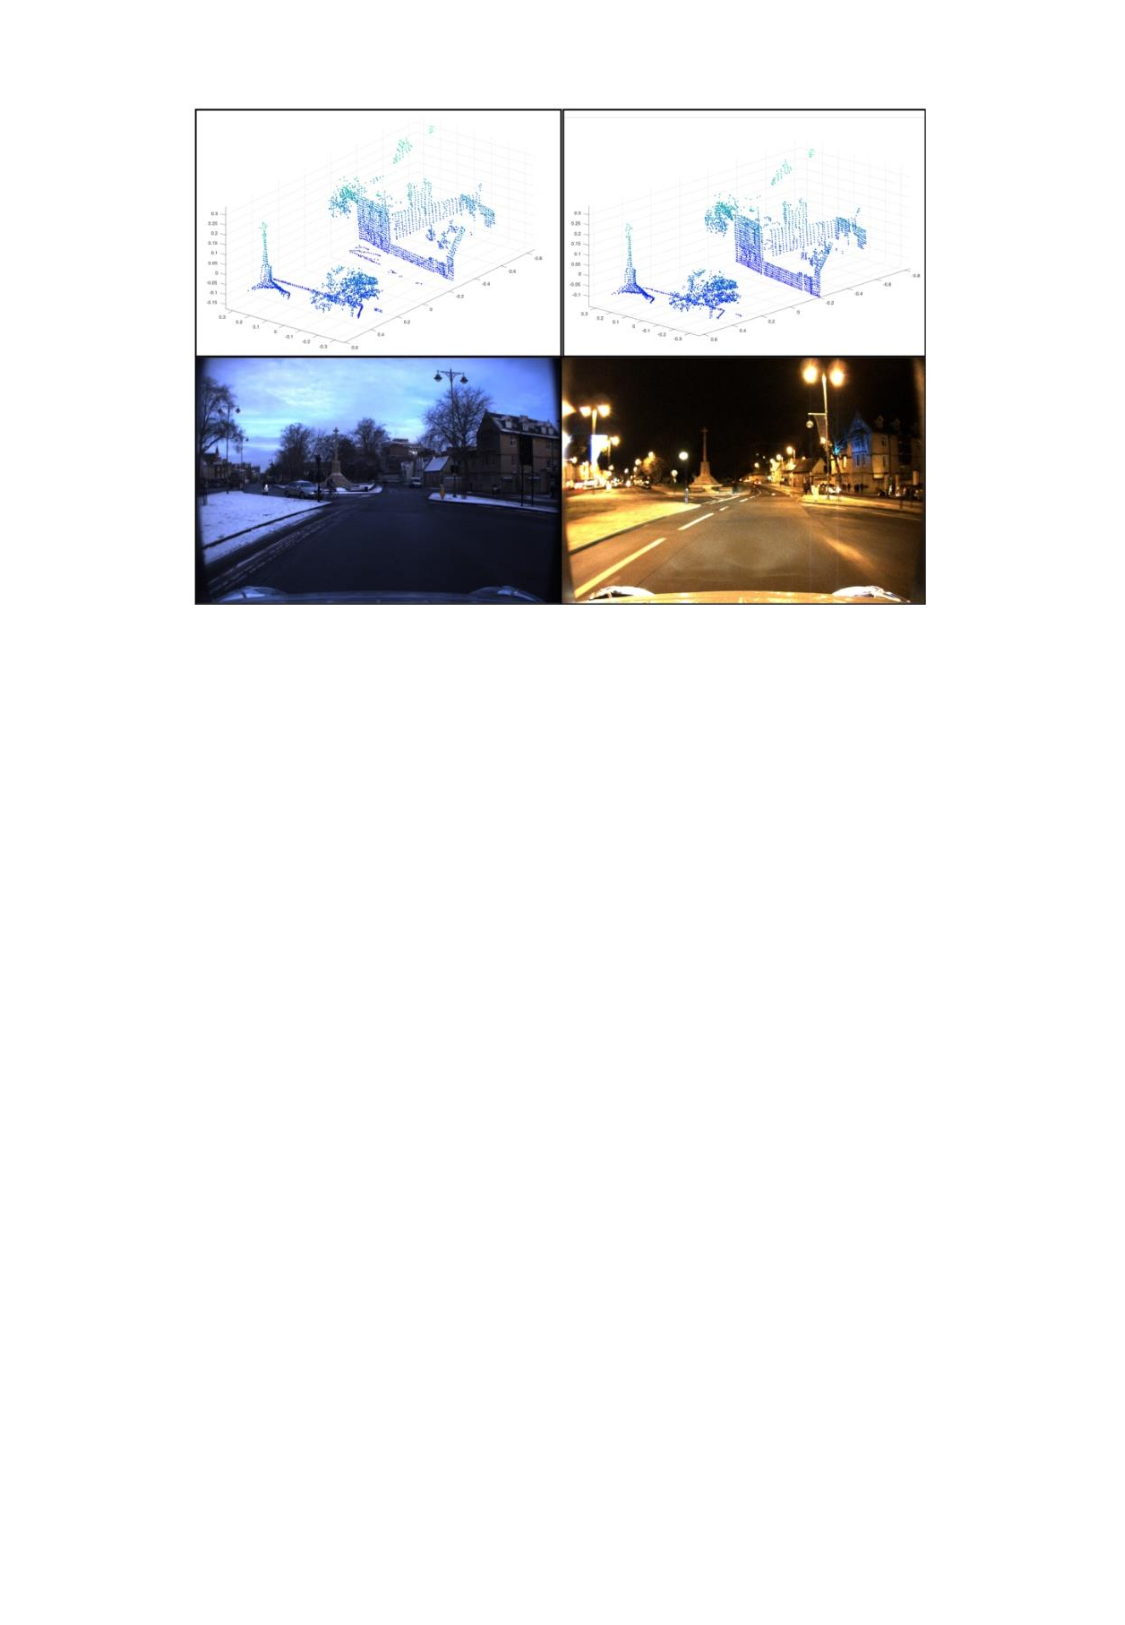
\includegraphics[width=\textwidth]{my/figure/1-1.pdf}
    \bicaption[\xiaosi 不同时间同一场景的点云与图像对比]
    {\wuhao 不同时间同一场景的点云与图像对比\upcite{PointNetVLAD}}
    {\wuhao Comparison between point cloud and image of the same scene at different time\upcite{PointNetVLAD}}
    \label{fig:1-1} 
\end{figure}
\vspace{-0.35cm}

在医疗领域,使用点云配准能够将患者的器官及内脏等组织融合成一个整体构建三维模型,辅助医生诊断。在文物修复领域,研究人员能过够对大型文物多次扫描后将其配准生成完整的文物模型,不仅能够存储文物的三维数据以实现文物的数字化存储,还能够为后续文物的保护和修复提供可靠的数据\upcite{文物}。在工业领域,点云配准是逆向工程的重要一环,能够为研究人员提供产品模型的三维数据\upcite{逆向工程}。更重要的是,点云配准是许多机器人任务的关键组成部分,是机器人对环境感知的重要一环\upcite{Map-matching}。在同时定位与建图(Simultaneous Localization And Mapping,SLAM)中,点云配准可以构建用于自动驾驶的路径规划和决策的三维地图\upcite{LCDNet}。点云配准也广泛应用于位置识别,它能够将实时的三维视图匹配到所属的三维地图中,以实现机器人对自身位置的定位\upcite{LPD}。同时点云配准在机器人的姿态估计中也发挥着不可或缺的作用。通过对齐视图与环境,可以获取机器人手臂的姿态信息,进而决定下一步该如何移动以抓取物体\upcite{2015review}。

点云配准是三维图形学研究的一个重要研究课题,也是计算机视觉的重要分支,其目的是将两个具有部分重叠区域的点云,经过一个变换矩阵在同一个坐标系下对齐。早期,不少学者提出了许多不同的方法来解决点云配准问题,这些方法主要针对于实验室理想环境下的合成数据集,而这些数据集也往往由单一的物体模型而不是场景构成。随着社会的发展,这些方法已经不能够满足生产生活需要。近年来越来越多的工作开始关注真实环境下的点云配准,其中基于深度学习的点云配准方法有着突出的表现。最近,针对低重叠率情况的点云配准得到了学界的广泛关注。所谓低重叠率的点云配准指的是将两个至多只存在30\%重叠区域的点云进行对齐。相比于一般情况的点云配准,低重叠率的点云对之间存在许多相似非重叠区域,这会很大程度上增加特征搜索寻找正确点对应的难度,导致大量非匹配区域的误匹配。由此可见低重叠情况下的点云配准的研究重点在于如何将点的对应关系聚集在重叠区域和如何增加相似区域的特征差异。

综上所述,点云配准是处理点云数据的一项基本任务,是推进自动化进程的关键一环,在生产生活中扮演着重要的角色。因此,研究点云配准算法,提高配准精度和减少算法时间复杂度具有重大的研究价值。同时,随着近年来人工智能深度学习的快速发展,基于深度学习的点云配准方法也取得了巨大成功。本文通过对现有方法研究进行分析并改进,提高在低重叠度的情况下点云配准算法的成功率。
% 由于传感器的视野有限,单次扫描只能捕捉一定空间的信息。因此将两个点云对齐的点云配准算法是正确处理点云数据基础。在点云配准中有两个相互关联的子问题:找到使两个点云对齐的刚性变换和找到两个点云之间点对点的对应关系。虽然在已知其中某个子问题的解时,另一个子问题很容易求解,但要同时求解两个子问题是比较困难的。尤其存在异常值时,点云配准将变得更加困难。其中异常值是指部分点在另一个点云中没有对应的点。异常值可能来自于用于收集点云的传感器的不完善或两个要配准的点云没有完全重叠的情况。

\section{国内外研究现状}
本节将从传统点云配准方法和基于深度学习的点云配准方法两个方向介绍点云配准方法的研究现状。其中传统点云配准方法早在上世纪90年代就得到了初步发展,而后在研究人员的不懈努力下传统方法的点云配准现在已经广泛应用于工业生产领域。随着近些年来的人工智能的发展,将点云配准与与深度学习融合也逐渐受到越来越多的研究人员的关注,并且其性能上已经超过传统的点云配准方法。

    \subsection{传统点云配准方法}
    迭代式最近点法\upcite{ICP}(Iterative Closet Points,ICP)是传统点云配准方法中最典型的一类,它由BESL等人在1992年提出。ICP方法通过计算源点云和目标点云原始点之间的欧氏距离,以最临近点作为对应点确定两点云间点的对应关系。然后,在已知点的对应关系时,通过基于奇异值分解法求解两点云之间的变换矩阵,并进行单次对齐。重复上述两个步骤直至满足预设要求完成整个配准过程。当源点云与目标点云之间具有良好的初始位姿时,ICP方法可以取得良好的配准结果。但是,当二者之间的距离较大时,该算法往往会在局部最优点处收敛,导致最终的结果不能满足实际生产生活需要。文献\cite{1998}提出一种模拟退火算法将ICP算法中根据点到点的距离确定的“硬”匹配关系转化为一种“软”匹配方式。这种方法虽然不能完全避免局部最优解问题,但是能够使算法在一定程度上得到缓解。YANG等人\upcite{Go-ICP}为了解决上述问题,提出一种全局最优的迭代式最近点算法(Globally Optimal Iterative Closet Point, Go-ICP),其基本思想是通过分支界定法跳出局部最优解,以实现全局最优解,但与此同时算法的速度严重下降。

    基于图的配准是另一类常见的方法,它主要是寻找更加准确的对应关系。相比于ICP方法中直接选取最邻近点作为对应点,基于图的配准方法将同时考虑点和边的关系。具体而言,图匹配算法不仅要求匹配点的点相似度高,而且要求节点之间的连线即边的相似度也要高。这种关系能够找到更准确的对应关系,而精确的对应关系有助于更好的变换估计。图匹配的优化属于二次分配问题,是一个典型的NP难问题,解决思想主要采取近似策略逼近。文献\cite{Almohamad}和文献\cite{CSGM}采用线性规划来解决图匹配问题。文献\cite{FGM}则将较大的相似矩阵分解为若干较小矩阵,这些矩阵对每个图的局部结构和相似性进行编码,解耦节点和边之间的相似性,使得求解过程简化。LERDEANU等人\upcite{Leordeanu}提出了一种谱松驰的方法来近似二次分配问题,它指出正确的对应能够形成强关联的集群,而错误的对应只是一种偶然,因此不太可能产生强关联的簇,根据这一特性能够有效找出正确的对应关系。

    高斯混合模型(Gaussian Mixture Models, GMM)是另一种常见的点云配准方法,它的核心思想是将配准问题中变换估计问题转化为求解点云数据的最大似然估计问题。任意两点之间的对应关系,将由原来的“硬”匹配转化为了由置信度表示的“软”匹配,但也因此其时间复杂度大大增加了。JRMPC等人\upcite{JRMPC}提出了一个EM算法,它估计了GMM参数以及将每个独立集合映射到“中心”模型上的旋转和平移。文献\cite{CPD}通过最大似然估将源点云数据拟合到目标点云。使源点云作为一个整体移动,以保持点集的拓扑结构。通过对具有刚性参数的GMM质心位置的重新参数化来施加一致性约束,并推导出EM算法的最大步骤的封闭解。文献\cite{CH-GMM}提出了一种新的凸包索引高斯混合模型。该模型通过计算每个点集凸包上的加权高斯混合模型响应来工作。

    传统的点云配准算法的优点有两个方面:(1)严格的数学理论可以保证算法的收敛性;(2)不需要训练数据。然而这类方法的局限性也较为明显:ICP算法需要一个较好的初始位置才能有良好的表现,这在真实场景下尤其是低重叠情况下难以达到要求;这类方法对数据的离群值、噪声和点云密度等特点较为敏感,在真实场景下的表现远没有在合成数据上的表现好。

    \subsection{基于深度学习的点云配准方法}
    基于深度学习的点云配准方法大致可以分为两类:端到端的点云配准方法和基于对应关系的点云配准方法。\par
    \subsubsection{端到端的点云配准方法}
    文献\cite{PointNetLK}提出的PointNetLK可以被认为是一个可学习的函数。因此,将用于图像对齐的经典视觉算法Lucas-Kanade\upcite{LucasKanade}(LK)算法与其相结合,并融合为一个循环深度神经网络。
    文献\cite{PPF}赋予PPF-FoldNet自动编码器(Auto Encoder,AE)一个姿态差异结构,其中两者之间的差异产生特定于姿态的描述符。在此基础上,引入了相对姿态估计网络RelativeNet,为关键点分配对应特定的方向。最后,利用一个简单而有效的假设-验证算法来快速预测和对齐两个点云。
    % 文献\cite{PCRNet}提出了PCRNet用来比较源点云和目标点云的全局特征。根据点云的物体形状的先验信息,生成特定形状包括不可见的形状,并使用带有全连接层的暹罗架构增加网络的鲁棒性。
    FMR\upcite{FMR}借鉴了PointNetLK的思想,利用刚性变换的可逆特性,采用编解码器结构监督全局特征。
    文献\cite{OMNet}提出了一种基于全局特征的迭代网络OMNet,用于部分重叠点云的配准。OMNet以由粗到细的方式学习掩码来拒绝非重叠区域,这将部分重叠的配准转换为相同形状的配准。此外,它提出了一种更实用的数据生成方式,其中CAD模型对源点云和参考点云进行两次采样,避免了普遍存在的过拟合问题。
    \vspace{-0.1cm}
    \begin{figure}[h]
        \centering 
        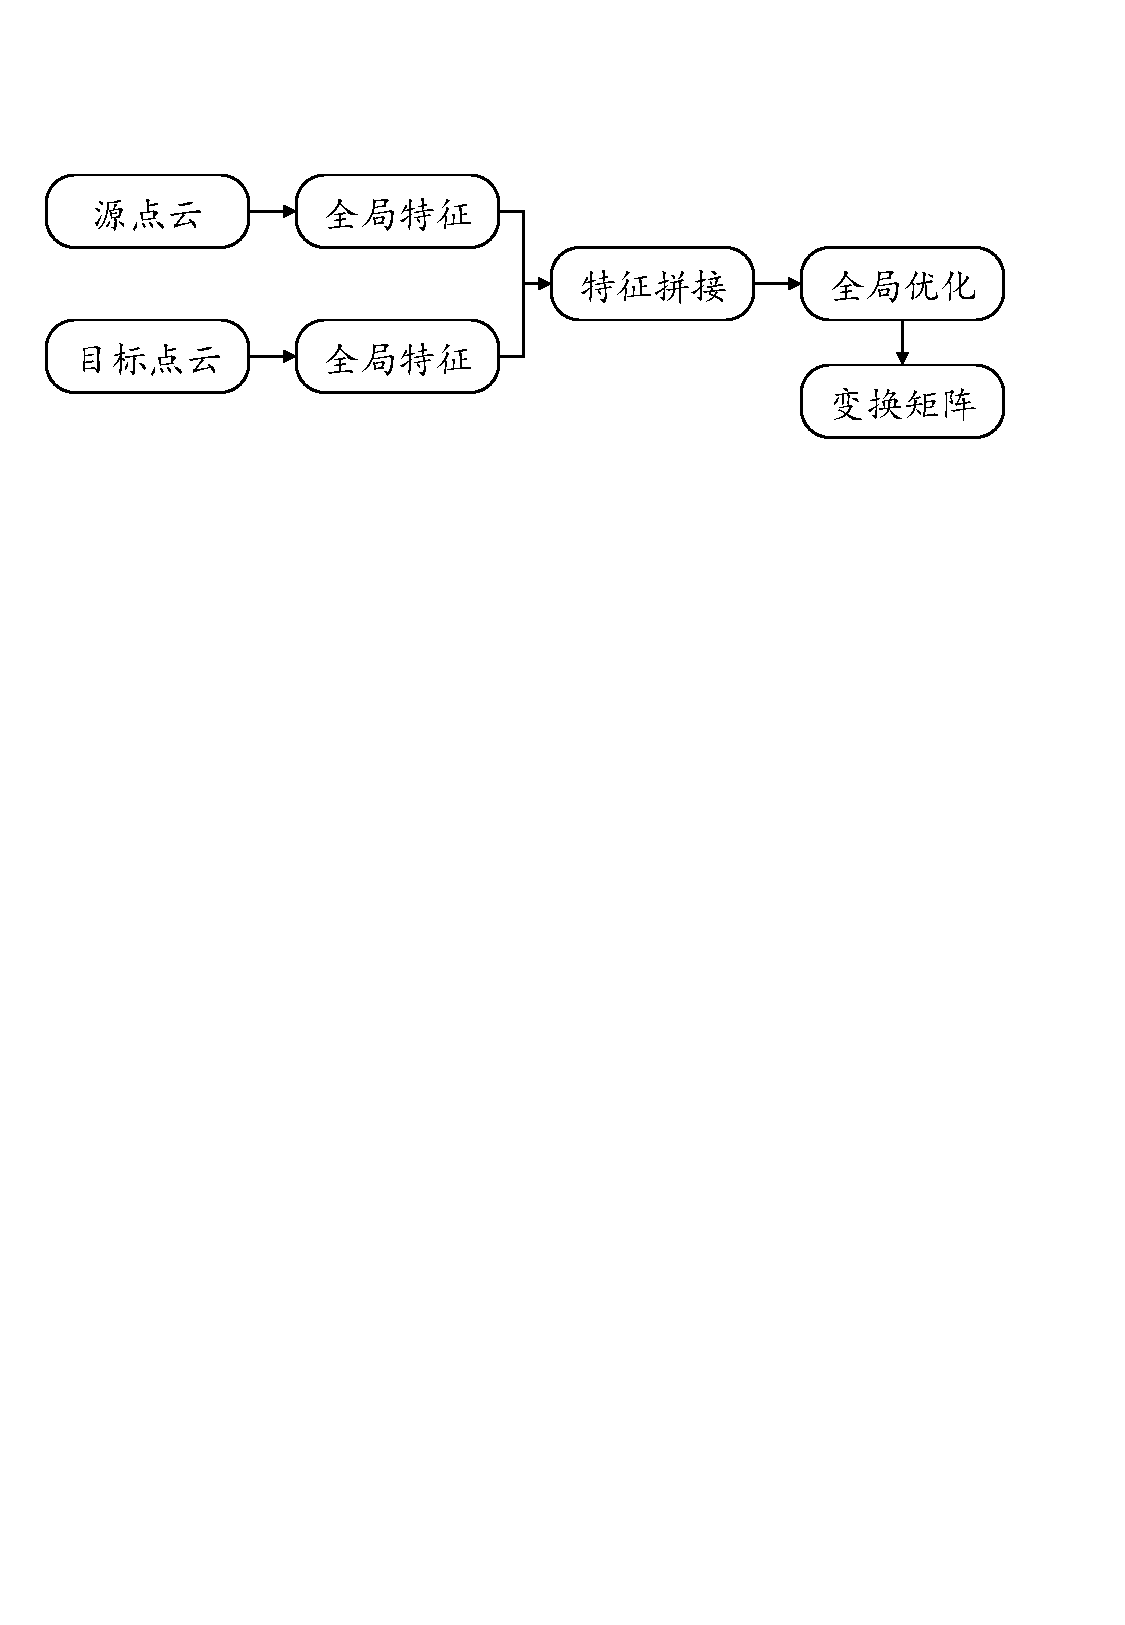
\includegraphics[width=12cm]{my/figure/1-2.pdf}
        \bicaption[\xiaosi 端到端的点云配准方法流程图]{\wuhao 端到端的点云配准方法流程图}{\wuhao Flowchart of the end-to-end point cloud registration}
        \label{fig:1-2} 
    \end{figure}
    \vspace{-0.2cm}
    % Deng等人将PPF特征和点云分别输入到PPF-foldnet和PC-FoldNet网络中,得到包含结构和姿态的新特征,并使用RelativeNet预测相对姿态。
    % PCRNet在拼接两个点云的全局特征后,使用类似于Siamese的网络来预测变换矩阵。FMR借鉴了PointNetLK的思想,利用刚性变换的可逆特性,采用编解码器结构监督全局特征。
    % Xu等人提出OMNet在迭代过程中预测源点云和目标点云的重叠掩码,通过mlp从两者的全局特征预测刚性转换。然而,直接配准方法在处理真实场景时往往受到限制。

    \subsubsection{基于对应关系的点云配准方法}
    基于对应关系的配准方法主要集中在四个方面:特征提取、关键点检测、异常值去除和位姿估计。
    QI等人先后提出了PointNet\upcite{PointNet}和pointnet++\upcite{PointNet++}。这两种方法虽然为点云的特征提取提供了参考,但都没有考虑点云的几何结构特征。
    文献\cite{3DFeat-Net}提出了一种利用弱监督学习三维特征检测器和描述子进行点云匹配的3DFeat-Net。与许多以往的工作不同,该方法不需要手动标注匹配的点。相反,可以利用对齐和注意力机制从全球定位系统(Global Positioning System,GPS)标记的3D点云中学习特征对应关系,而无需人工标注。
    文献\cite{PerfectMatch}提出了3DSmoothNet,它利用暹罗网络架构匹配3D点云,并使用体素化平滑密度值表示实现全卷积层,并与局部参考系对齐以实现旋转不变性。
    文献\cite{DGCNN}提出了一种新的神经网络模块EdgeConv,构造了DGCNN来捕获点之间的拓扑信息。EdgeConv作用于网络每一层中动态计算的图,其中包含了局部邻域信息,并可以叠加应用于学习全局形状属性。
    文献\cite{KPConv}提出KPConv来模拟二维卷积中的运算,以更好地捕获局部几何信息。
    文献\cite{3DMatch}提出的3DMatch网络以体素为输入,利用三维卷积神经网络学习局部几何特征。
    文献\cite{FCGF}提出全卷积几何特征采用稀疏三维卷积代替传统的三维卷积来缓解点云稀疏性带来的问题。
    SpinNet\upcite{SpinNet}通过估计的参考轴约束z轴自由度,并使用球面体素化消除XY平面旋转自由度,提取具有高鲁棒性的特征。
    文献\cite{D3Feat}提出的D3feat在提取点云特征时使用KPConv组成的U-Net网络来检测关键点,并使用密度不变显著性评分来缓解密度对显著性的影响。
    文献\cite{PREDATOR}提出了一种点云配准模型Predator,该模型对重叠区域进行了深度关注。与以前的工作不同,该模型是专门设计来处理低重叠的点云对的。其核心思想是在两个点云的潜在编码之间进行早期信息交换的重叠注意块,以预测哪些点不仅是显著的,而且还位于两个点云之间的重叠区域。
    
    \vspace{-0.1cm}
    \begin{figure}[h]
        \centering 
        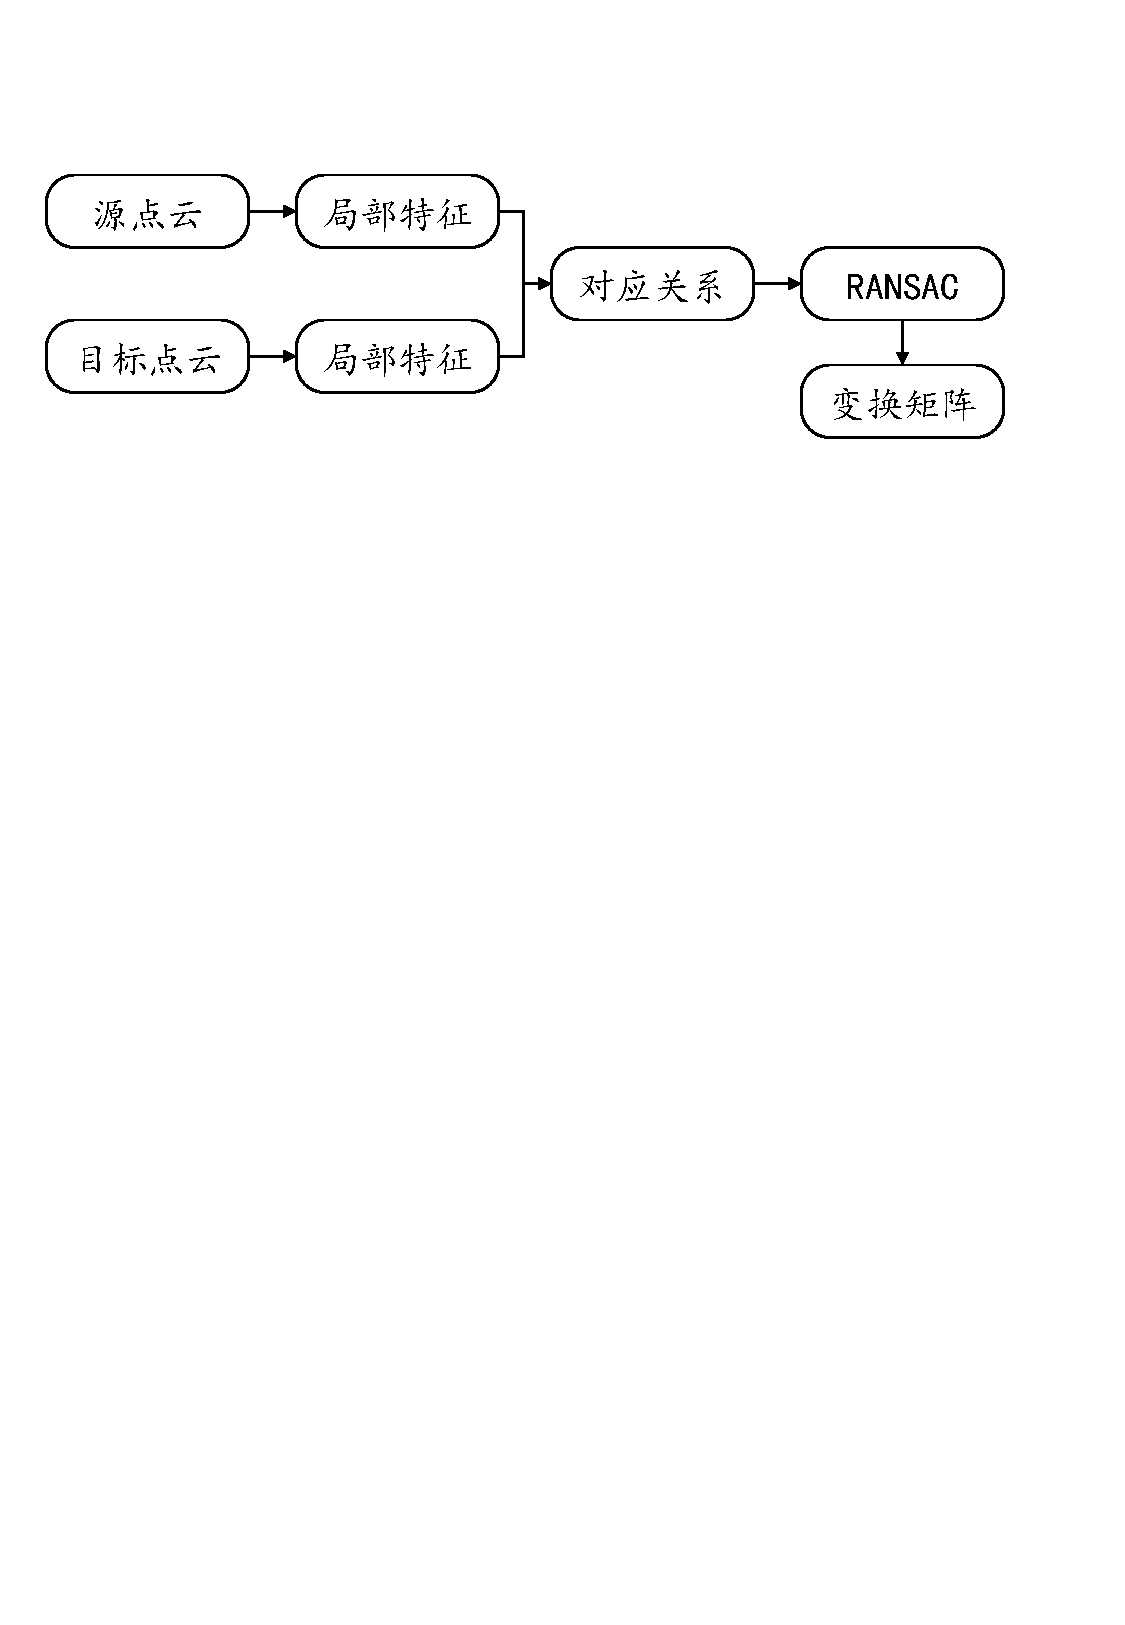
\includegraphics[width=12cm]{my/figure/1-3.pdf}
        \bicaption[\xiaosi 基于对应关系的点云配准方法流程图]{\wuhao 基于对应关系的点云配准方法流程图}{\wuhao Flowchart of point cloud registration method based on correspondence}
        \label{fig:1-3} 
    \end{figure}
    \vspace{-0.35cm}

    文献\cite{PointDSC}提出PointDSC,将传统方法中的空间几何一致性约束添加到网络中,利用神经网络提取对应关系的特征,通过可微的光谱匹配模块,对成对的空间一致性监督,以估计每个对应的嵌入特征的置信度。
    文献\cite{DCP}提出一个由点云嵌入网络、结合注意力模块近似组合匹配层、可微奇异值分解层三部分组成的DCP网络,解决局部最优和ICP方法中的其他问题。
    IDAM\upcite{IDAM}包括一个迭代的距离感知相似矩阵卷积模块,将来自特征和欧几里得空间的信息合并到成对点匹配过程中。这些卷积层学习基于整个几何特征的联合信息和每个点对的欧几里得偏移来匹配点,克服了通过简单地使用特征向量的内积来匹配的缺点。
    文献\cite{DGR}提出了一个可微分的框架DGR。它由三个模块组成:用于对应置信度预测的6维卷积网络,用于封闭姿态估计的可微分加权Procrustes算法,以及用于姿态细化的鲁棒基于梯度的SE(3)优化器。
    % \vspace{-0.1cm}
    % \begin{figure}[h]
    %     \centering 
    %     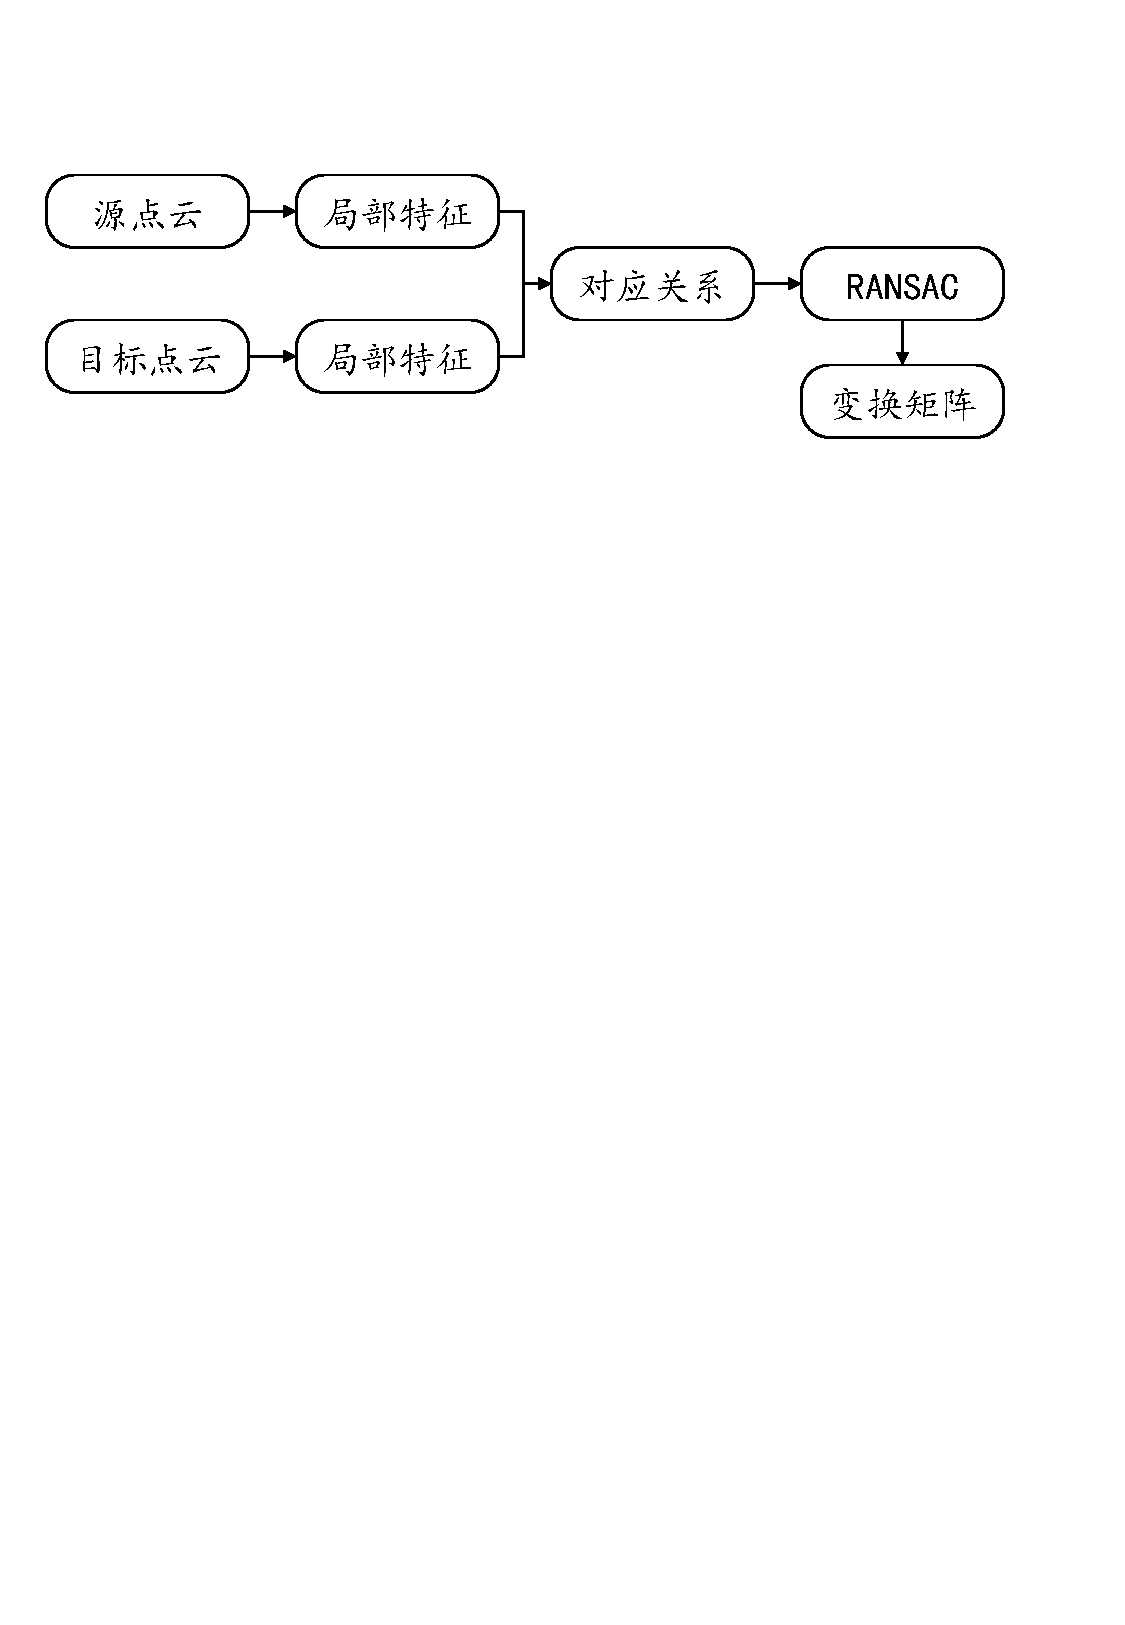
\includegraphics[width=12cm]{my/figure/1-3.pdf}
    %     \bicaption[\xiaosi 基于对应关系的点云配准方法流程图]{\wuhao 基于对应关系的点云配准方法流程图}{\wuhao Flowchart of point cloud registration method based on correspondence}
    %     \label{fig:1-3} 
    % \end{figure}
    % \vspace{-0.35cm}
    % Deng等人提出PPFNet,将点对特征(PPF)与点网相结合,提高了特征对噪声的鲁棒性。
    % Yew和Lee等人提出的3DFeatNet利用弱监督深度网络解决了点云数据精确标注的难题,提高了特征质量。
    % Gojcic等人提出了3DSmoothNet,它利用暹罗网络架构来编码光滑密度值体素化。
    % Wang等人设计了边缘卷积(EdgeConv)运算,构造了DGCNN来捕获点之间的拓扑信息。
    % Thomas等人提出KPConv来模拟二维卷积中的运算,以更好地捕获局部几何信息。
    % Zeng等人提出的3DMatch网络以体素为输入,利用三维卷积神经网络学习局部几何特征。
    % Choy等人提出FCGF采用稀疏三维卷积代替传统的三维卷积来缓解点云稀疏性带来的问题。
    % SpinNet通过估计的参考轴约束z轴自由度,并使用球面体素化消除XY平面旋转自由度,提取具有高鲁棒性的特征。
    % Bai等人提出的D3feat在提取点云特征时使用KPConv组成的U-Net网络来检测关键点,并使用密度不变显著性评分来缓解密度对显著性的影响。
    % Huang等在将任务扩展到低重叠场景的同时,通过检测重叠区域中点的可能性,提高了正确检测的概率。
    % Bai等提出PointDSC,将传统方法中的空间几何一致性约束添加到网络中,利用神经网络提取对应关系的特征,选择一组空间一致的点对。
    % DCP(深度最近点)和DeepVCP采用加权置信度估计相对位姿。
    % IDAM(迭代距离感知相似矩阵)和DGR(深度全局配准)通过选择高置信度点对,采用加权SVD求解刚性变换。
    \subsection{存在的问题}
    点云配准方法的研究已经有了二十多年的发展并且取得了一系列的成就,特别是在深度学习流行起来之后,许多研究利用深度神经网络取得了不错的成果。然而,在最近的相关文献\cite{Dope}中已经提到这些基于深度学习的方法的主干网络往往会遇到高层特征的过度平滑和结构模糊性相关的难以区分的特征问题,这是点云配准的一个关键瓶颈。它们忽略了特征提取的一个关键因素,这可能严重影响配准精度:源点云和目标点云中每个点特征的独特性;也就是说,为了获得精确的点对应关系,以估计最优刚性变换,所需的点特征应该充分表示任何给定点附近的几何模式,同时仍然与同一点云中围绕其它点的局部结构特征有足够的差异性。然而,许多工作\upcite{Deeper,Measuring}使用的骨干网络容易导致特征的超平滑和结构性的模糊问题,导致点特征难以区分。同时,将图像数据中的颜色和纹理信息引入进来通过多模态的融合,增加点特征之间的差异性是一个简单有效的想法。但是在相关研究中,许多多模态融合的方法并没有显示出比单模态的方法更加优异的表现。如何更有效的融合点云和图像两种模态的特征也是一个值得研究的问题。

\section{论文研究的主要内容}
本研究分别从嵌入几何结构和多模态融合两个方面入手,提高特征间的差异性,提出如下两个点云配准的方法。\par
1.基于显著锚点几何嵌入的点云配准方法。首先使用共享参数的骨干网络来提取源点云和目标点云的局部特征,在特征提取过程中同时对点云下采样进行超点聚合。之后在超点层面选取出若干分布于重叠区域的特征显著的锚点。同时,提出了一种新颖的基于注意力机制的几何嵌入方法。它的核心思想是将每个超点与锚点间的距离与角度信息进行编码,由于选取的多个锚点在空间中保持了一定的几何结构,因而使得这些超点与锚点之间的几何编码能够给每个超点带来各不相同的差异性特征。然后通过一个迭代优化模块,选取出更加显著的锚点进一步作结构嵌入增加特征差异性,并形成最终的超点对应。这些超点在物理空间中表示一个连续空间的区域,通过上采样能够建立超点与原始点之间的包含关系。这种由粗到细的配准方法可以在对应区域内部寻找点的对应关系而无需在全局点云中寻找,能够有效缓解特征平滑带来的误匹配,进而在变换估计中产生更加准确的变换矩阵。\par
2.基于多模态特征融合的锚点定位点云配准方法。现有的点云和图像两种模态融合方法往往通过对图像进行特征提取之后,将其与点云进行简单拼接并送入神经网络完成特征融合。与这些方法不同的是,本方法采用一种对齐策略,利用相机参数将点云和图像完成点与像素的对齐之后分别提取点云特征和图像特征。并利用点与像素之间的对应关系,通过交叉注意力机制完成像素到点的选择性融合。在此过程中,两种模态的特征均会被映射至模态无关与模态相关的两个特征子空间。在模态无关子空间中,点云和图像完成模态间特征的融合,随后将融合后的特征与点云在模态相关子空间中的投影相融合。这种方法能够有效减少点云和图像之间的域间隙,使得融合过程既不过多的引入噪声也不丢失互补信息,形成最终的超点特征中。
% 随着深度学习的蓬勃发展,通过学习到的特征\cite{D3Feat}、\cite{FCGF}进行对应搜索,无需迭代,通过一阶段估计(如RANSAC\cite{RANSAC})完成转换。根据学习到的特征,对源点云和目标点云中的一组关键点进行检测和匹配,进行配准\cite{D3Feat}、\cite{Graphite}。然而,由于源点云与目标点云之间存在非重叠区域的重复模式和重叠部分的低几何区域,因此精确提取源点云与目标点云之间的可重复兴趣点并非易事。如图1所示,源和目标包含重复的沙发,这些沙发在不重叠的区域外观相似。重复的模式容易产生不正确的对应关系。此外,对于重叠区域的低几何部分,例如由平面组成的楼层,很难获得准确的对应关系,因为可以提取的特征很少。这些问题对定位精确的点对应并进行可靠的配准提出了巨大的挑战,在室内情况下尤其突出。\par
% 本文首先通过聚合原始点获得超点,然后利用超点的特征进行区域匹配。在相应区域内,进一步得到点对应关系进行变换估计。利用注意机制\cite{attention}将全局上下文合并为特征,实现更好的超点匹配。给定一个超点,所有其他超点的几何信息被无差别地嵌入到特征\cite{Geometric}中。然而,点云通常存在弱几何和重复模式。在这种情况下,周围的斑块往往充满了相似的几何结构,而模糊的几何结构的加入,并不能帮助区分低几何和重复区域的超点,导致斑块对应不正确。\par
% 因此,在本文中,提出了一种鲁棒点云配准方法。一组对应的包含相对丰富的判别几何信息的超点被定位为显著锚点。由于突出锚点与正确的超点对应点之间的几何信息是一致的,因此突出锚点的几何嵌入可以有效地剔除异常值,在几何难度较大的区域获得准确的对应点。具体来说,我们首先对源点和目标点进行下采样,形成超点,并联合学习相关特征。我们首先设计了一个锚点定位模块,利用非最大抑制来获取源点云和目标点云上分布稀疏且具有代表性的锚点。\par
% 通过显著锚定,我们提出了一种选择性几何嵌入模块,增强了超点特征,以实现精确的补丁匹配。我们利用注意机制,有选择地嵌入突出点的几何信息,而不是聚集周围超点的所有几何信息。点云内的超点距离采用自注意结构嵌入。利用结构交叉注意技术,将超点、距离、角度等选择性几何信息纳入系统。为了获取最有效的突出点和显著特征,迭代更新突出点和超点特征的位置,这对于获得精确的超点对应关系起着至关重要的作用。最后,利用姿态估计器建立点间的对应关系来生成最终的变换。\par

%     \begin{itemize}
%     \item 我们提出了一个健壮的点云配准框架,通过嵌入显著锚的几何结构,能够实现具有低几何结构和重复模式的点云配准的最先进性能。
%     \item 我们设计了一种选择性几何结构嵌入方法,通过在超点和突出锚点之间嵌入几何信息来增强超点特征的区别。
%     \item 我们提出了一种突出锚的定位和更新方法,以获得在源点云和目标点云的重叠区域中分布稀疏且包含丰富的判别几何信息的最有效的突出锚。
%     \end{itemize}

\section{论文组织结构}
为了更加清晰地阐述本文的主要工作,本文结构安排如下:

第1章为绪论部分。首先对本文的选题背景和研究意义进行了介绍。然后,对国内外学者在点云配准研究领域取得的一些成就和研究进展进行了简单的陈述,并对目前点云配准方法中存在的问题进行了分析探讨。最后,对本文的主要研究做了简单的介绍,并阐述了本文的组织结构。

第2章为相关技术理论基础。首先对点云配准任务进行介绍。然后,介绍了点云配准任务中常用的用于求解刚体变换矩阵的基于SVD的线性代数法和基于RANSAC\upcite{RANSAC}的随机一致性采样法。接着,对点云配准的数据集做了详细介绍,主要包括合成数据集和真实场景数据集。最后,介绍了用于评估点云配准算法的性能的评价指标。

第3章是基于显著锚点几何嵌入的点云配准方法。首先介绍了本文提出方法的主要动机。接下来介绍了基于显著锚点几何嵌入的框架网络,介绍了如何从下采样后的超点中选取出位于重叠区域的保持一定几何结构的显著锚点。接下来介绍了如何利用自注意力和交叉注意力机制嵌入超点与超点之间以及超点与锚点之间的几何结构特征。之后对基于由粗到细框架的点云配准方法的点匹配阶段和变换估计方法做了简单介绍。接着介绍了该网络分别用来监督粗匹配阶段产生的超点匹配结果与细匹配阶段产生的点匹配结果的两个损失函数。然后是实验部分,对实验用到的数据集,实验设置以及实验结果及分析做了详细的描述。最后对第三章进行了总结。

第4章是基于多模态的锚点定位点云配准。首先介绍了当前方法将点云与图像两种模态融合的一些问题和多模态融合之前加入对齐模块的动机。然后简要介绍了本文对点云和图像两种模态数据进行特征提取的网络结构。之后介绍了对齐模块在整个网络中的作用与功能,主要是消除在数据增强情况下点云和图像数据的错位。然后介绍了多模态融合模块,利用一个简单的映射网络将两种模态的特征在模态无关子空间进行融合,并在模态相关子空间进一步补充相关信息的过程。接下来是实验部分,从数据集的预处理,实验设计和结果分析三个方面来进行阐述。最后对本章进行了总结。

第5章是总结与展望。首先对本文所作的工作进行了总结,然后根据本文的实验结果指出了方法中存在的问题和未来的研究方向。

\clearpage

% 第2章
\chapter{点云配准相关理论}
\thispagestyle{others}
\pagestyle{others}
\xiaosi

\section{本章引言}
首先,本章将对数字空间如何表示三维空间的物体及运动做出简要介绍,这是研究点云配准方法的前提。同时,当前点云配准方法与人工智能相关技术深度融合,因此本章将对深度神经网络作出必要介绍,这是研究点云配准方法的基础。之后,本章将介绍若干用于评估算法性能的公开数据集,包括合成数据集和真实场景数据集,这是验证点云配准算法的基础。最后,本章将对用于评价算法优劣的各项指标做出简要介绍。

\section{刚体变换基础}
    \subsection{表示形式}
    \subsubsection{变换矩阵}
    三维变换最常见的表示是变换矩阵,三维变换矩阵由旋转和平移两部分组成。首先在只考虑旋转变换的情况下,对于任意向量$\mathbf{a}$而言,已知它在两个单位正交基$\mathbf{(e_1,e_2,e_3)}$,$\mathbf{(e'_1,e'_2,e'_3)}$下的坐标分别是$(a_1,a_2,a_3)$,$(a'_1,a'_2,a'_3)$, 其中$\mathbf{(e'_1,e'_2,e'_3)}$由$\mathbf{(e_1,e_2,e_3)}$经过旋转得到。因为向量本身并没有发生变化,所以可以用公式(2-1)表示$\mathbf{a}$与$\mathbf{a'}$之间的关系:
    \begin{equation}
        \begin{bmatrix}
            \mathbf{e_1},\mathbf{e_2},\mathbf{e_3}
        \end{bmatrix}
        \begin{bmatrix}
            a_1 \\ a_2 \\ a_3
        \end{bmatrix}
        =
        \begin{bmatrix}
            \mathbf{e'_1},\mathbf{e'_2},\mathbf{e'_3}
        \end{bmatrix}
        \begin{bmatrix}
            a'_1 \\ a'_2 \\ a'_3
        \end{bmatrix}
    \end{equation}
    对公式(2-1)的左右两边同时左乘$\mathbf{(e_1,e_2,e_3)}^\mathrm{T}$,将左边系数矩阵化简为单位矩阵可以得到公式(2-2),它表示了坐标$(a_1,a_2,a_3)$与坐标$(a'_1,a'_2,a'_3)$之间的转换关系:
    \begin{equation}
        \begin{bmatrix}
            a_1 \\ a_2 \\ a_3
        \end{bmatrix}
        =
        \begin{bmatrix}
            \mathbf{e}^T_1 \mathbf{e}'_1 & \mathbf{e}^T_1 \mathbf{e}'_2 & \mathbf{e}^T_1 \mathbf{e}'_3\\
            \mathbf{e}^T_2 \mathbf{e}'_1 & \mathbf{e}^T_2 \mathbf{e}'_2 & \mathbf{e}^T_2 \mathbf{e}'_3\\
            \mathbf{e}^T_3 \mathbf{e}'_1 & \mathbf{e}^T_3 \mathbf{e}'_2 & \mathbf{e}^T_3 \mathbf{e}'_3\\
        \end{bmatrix}
        \begin{bmatrix}
            a'_1 \\ a'_2 \\ a'_3
        \end{bmatrix}
    \end{equation}
    将公式(2-2)右边的系数矩阵称为旋转矩阵$\mathbf{R}$。旋转矩阵由两组基之间的内积组成,能够表示任意向量在旋转前后的坐标变化关系。可以注意到旋转矩阵是正交矩阵,因此上述旋转变换的逆变换可由公式(2-3)表示:
    \begin{equation}
        \mathbf{a'} = \mathbf{R}^{-1}\mathbf{a} = \mathbf{R}^{\mathrm{T}}\mathbf{a}
    \end{equation}
    为了更准确的描述刚体在三维空间中的运动,现在将平移分量$\mathbf{t}$引入进来,公式(2-4)表示了物体的旋转和平移过程:
    \begin{equation}
        \mathbf{
        a = R a' + t
        }
    \end{equation}
    公式(2-4)虽然能够准确的表示刚体在三维空间中的单次运动变换,但是当需要连续表示多次变换时往往就会包含多个括号并显得不够简洁。故引入齐次坐标和变换矩阵,公式(2-4)的齐次表达式为公式(2-5):
    \begin{equation}
        \mathbf{
        \begin{bmatrix}
            \mathbf{a} \\ 1
        \end{bmatrix}
        =
        \begin{bmatrix}
            \mathbf{R}   & \mathbf{t}\\
            0^\mathrm{T} & 1
        \end{bmatrix}
        \begin{bmatrix}
            \mathbf{a'} \\ 1
        \end{bmatrix}
        }
    \end{equation}
    公式(2-5)等式左边第一个矩阵被定义为变换矩阵$\mathbf{Trans}$,它主要由表示旋转的旋转矩阵$\mathbf{R}$和表示平移的平移向量$\mathbf{t}$两部分组成。\par
    变换矩阵虽然能够精确的表示刚体在三维空间中的运动,但是这种表现形式也存在着某些局限性:(1)对于旋转矩阵而言,需要有9个变量描述物体在三维空间中的旋转,而旋转只存在3个自由度;对变换矩阵而言,则需要16变量表示物体的旋转和平移,即使这些运动只存在6个自由度。因此,以变换矩阵来表示物体在三维空间中的运动是冗余的,这也引出旋转矩阵的另一个局限性;(2)变换矩阵变量之间存在约束关系,由上述公式(2-2)可以看到变换矩阵的旋转矩阵部分是一个行列式为1的正交矩阵。这种约束关系对于变换矩阵的计算求解和优化而言会使得问题变得麻烦复杂。

    \subsubsection{旋转向量}
    旋转向量是表示刚体在三维空间中运动的另一种常见形式。它通过两个变量将三维空间中的旋转参数化,单位向量$\mathbf{n}$表示旋转轴的方向,角度$\theta$描述围绕旋转轴的旋转幅度。通过罗格里格斯公式可以完成旋转向量和变换矩阵之间的转化。对于任意向量$\mathbf{v}$绕单位向量$\mathbf{n}$旋转$\theta$角度后得到$\mathbf{v'}$。可以将向量$\mathbf{v}$相对于$\mathbf{n}$分解成平行分量$\mathbf{v_\parallel}$和垂直分量$\mathbf{v_\perp}$,由公式(2-6)表示:
    \begin{equation}
        \mathbf{
        v = v_\parallel + v_\perp
        }
    \end{equation}
    式中,平行分量$\mathbf{v_\parallel}$和垂直分量$\mathbf{v_\perp}$分别可以用公式(2-7)和公式(2-8)表示:
    \begin{equation}
        \mathbf{
        v_\parallel = (v \cdot n)n
        }
    \end{equation}
    \begin{equation}
        \mathbf{
        v_\perp = v - v_\parallel = v - (v \cdot n)n = -n\times(n\times v)
        }
    \end{equation}
    根据投影关系可以得到$\mathbf{v'}$和$\mathbf{v}$的平行分量和垂直分量之间的关系,分别用公式(2-9)和公式(2-10)表示:
    \begin{equation}
        \mathbf{v'_\parallel} = \mathbf{v_\parallel},
    \end{equation}
    \begin{equation}
        \mathbf{v'_\perp}=cos(\theta) \mathbf{v_\perp} + sin(\theta)\mathbf{n}\times \mathbf{v_\perp}
    \end{equation}
    又因为$\mathbf{n}$与$\mathbf{v'}$平行,因此可以进一步得到公式(2-11):
    \begin{equation}
        \mathbf{
        n\times v_\perp = n\times(v-v_\parallel)= n\times v - n\times v_\parallel = n\times v
        }
    \end{equation}
    将公式(2-11)代入公式(2-10)可知公式(2-12):
    \begin{equation}
        \mathbf{v'_\perp}=cos(\theta) \mathbf{v_\perp} + sin(\theta)\mathbf{n}\times \mathbf{v}
    \end{equation}
    进而$\mathbf{v'}$可由公式(2-13)表示:
    \begin{equation}
        \begin{aligned}
        \mathbf{v'}
    &    =\mathbf{v_\parallel} + cos(\theta)\mathbf{v_\perp} + sin(\theta)\mathbf{n}\times \mathbf{v}\\
    &    =\mathbf{v_\parallel} + cos(\theta)\mathbf{(v-v_\perp)} + sin(\theta)\mathbf{n\times v} \\
    &    =cos(\theta)\mathbf{v} + (1-cos(\theta))\mathbf{v_\perp} + sin(\theta)\mathbf{n\times v}\\
    &    =cos(\theta)\mathbf{v} + (1-cos(\theta))\mathbf{(n\cdot v)n} + sin(\theta)\mathbf{n\times v}
        \end{aligned}
    \end{equation}
    将公式(2-13)重新组合并化简可得到最终旋转向量与变换矩阵之间的关系,可以得到公式(2-14):
    \begin{equation}
        \mathbf{T} = cos(\theta)\mathbf{I} + (1-cos(\theta))\mathbf{n}\mathbf{n}^\mathrm{T} + sin(\theta)\mathbf{n}^\land
    \end{equation}

    \subsubsection{四元数}
    与变换矩阵和旋转向量相比,单位四元数是一种更加紧凑、高效且数值稳定的描述刚体在三维空间运动变换的表达形式。虽然,它并不直观,并且由于三角函数的周期性,不同的旋转角度可能会编码为相同的四元数。但是只要将其弧度限制在$[0,2\pi]$,四元数不失为一种良好的形式。单位四元数可以通过引入抽象符号$\mathbf{i,j,k}$来定义,它们满足规则$\mathbf{i^2=j^2=k^2=ijk=}-1$,同时满足除乘法交换律以外的常用代数规则。
    设$v=[0,\mathbf{v}], u=[0,\mathbf{u}]$,易得公式(2-15)与公式(2-16):
    \begin{equation}
        vu=[-\mathbf{v}\cdot \mathbf{u}, \mathbf{v}\times \mathbf{u}],
    \end{equation}
    \begin{equation}
        uv_\perp= [-\mathbf{u}\cdot \mathbf{v}_\perp, \mathbf{u}\times \mathbf{v}_\perp]
    \end{equation}
    又因为$\mathbf{v_\perp}$与$\mathbf{u}$正交,所以$\mathbf{u}\cdot \mathbf{v_\perp}=0$,将之带入公式(2-16),可得公式(2-17):
    \begin{equation}
        uv_\perp= [0, \mathbf{u}\times \mathbf{v}_\perp] = \mathbf{u}\times \mathbf{v}_\perp
    \end{equation}
    进一步可得到公式(2-18):
    \begin{equation}
        \begin{aligned}
        v'_\perp 
    &= cos(\theta) v_\perp + sin(\theta)(uv_\perp)\\
    &=(cos(\theta)+sin(\theta)u)v_\perp
        \end{aligned}
    \end{equation}
    令$q=cos(\theta)+sin(\theta)u$,可得$v'_\perp=qv_\perp$,令$q=p^2$,有$p=[cos(0.5\theta),sin(0.5\theta)\mathbf{u}]$。又因为$qq^{-1}=qq^*=1,qv_\parallel=v_\parallel q, qv_\perp= v_\perp q^*$,将其带入公式(2-13)可得公式(2-19):
    \begin{equation}
        v' = pvp^*=pvp^{-1}
    \end{equation}

    \subsection{变换矩阵求解}
    对于基于对应关系的点云配准方法而言,在得到源点云和目标点云之间的点对应关系之后,需要将这种点的对应关系转化成点云之间的变换矩阵,以得到的最终的配准结果。由于本文在不同阶段利用了奇异值分解法(SVD)和随机一致性估计法(RANSAC),本节将对这两种方法进行介绍。\par

    \subsubsection{奇异值分解法}
    设集合$\mathcal{C}=\{(\mathbf{p}_i,\mathbf{q}_i)|i=1,...,n\}$,其中$\mathbf{p}_i$是源点云$\mathcal{P}$中与目标点云$\mathcal{Q}$中的$\mathbf{q}_i$点相对应的点。在已知所有对应点的对应关系$\mathcal{C}$后,目标点云与源点云之间的变换问题可以表示成公式(2-20):
    \begin{equation}
        \mathbf{R},\mathbf{t} = \mathrm{argmin} \sum_{(\mathbf{p}_i,\mathbf{q}_i)\in \mathcal{C}}  \Vert \mathbf{q}_i-(\mathbf{R}\cdot \mathbf{p}_i + \mathbf{t}) \Vert^2
    \end{equation}
    对公式(2-20)右边求导并令其等于0有公式(2-21):
    \begin{equation}
        \begin{aligned}
        0 
        &= \sum_{i=1}^{n} 2(\mathbf{R} \mathbf{p}_i + \mathbf{t} - \mathbf{q}_i) \\
        &= 2n\mathbf{t} + 2\mathbf{R} (\sum_{i=1}^n \mathbf{p}_i) - 2\sum_{i=1}^n \mathbf{q}_i
        \end{aligned}   
    \end{equation}
    公式(2-21)左右边同时除以$n$并化简可以得到公式(2-22):
    \begin{equation}
        \begin{aligned}
        0 
        &= 2\mathbf{t} + \frac{2\mathbf{R}(\sum_{i=1}^n \mathbf{p}_i)}{n} -\frac{2\sum_{i=1}^n \mathbf{q}_i}{n}
        &= 2\mathbf{t} + 2\mathbf{R}\mathbf{\bar{p}} -2\mathbf{\bar{q}}
        \end{aligned}   
    \end{equation}
    式中,$\mathbf{\bar{p}}$和$\mathbf{\bar{q}}$分别是源点云和目标点云的形心。将公式(2-22)化简可得:
    \begin{equation}
        \mathbf{t} = \mathbf{\bar{q}} - \mathbf{R}\mathbf{\bar{p}}
    \end{equation}
    将公式(2-23)带入(2-20)可知公式(2-24):
    \begin{equation}
        \begin{aligned}
        \sum_{(\mathbf{p}_i,\mathbf{q}_i)\in \mathcal{C}}  \Vert \mathbf{q}_i-(\mathbf{R}\cdot \mathbf{p}_i + \mathbf{t}) \Vert^2
        &=
        \sum_{(\mathbf{p}_i,\mathbf{q}_i)\in \mathcal{C}}  \Vert (\mathbf{q}_i-\mathbf{\bar{q}})-\mathbf{R}(\mathbf{p}_i-\mathbf{\bar{p}}) \Vert^2\\
        &= 
        \sum \Vert \mathbf{R}\mathbf{p}'_i-\mathbf{q}'_i \Vert^2
        \end{aligned}
    \end{equation}
    根据矩阵Frobenius范数(F-范数)的定义,矩阵F-范数的平方可以转化成矩阵的内积形式,进而得到矩阵迹的表达形式,然后再带入公式(2-24)化简得到公式(2-25):
    \begin{equation}
        \sum_{(\mathbf{p}_i,\mathbf{q}_i)\in \mathcal{C}}  \Vert \mathbf{R}\mathbf{p}'_i-\mathbf{q}'_i \Vert^2
        =
        {\mathbf{p}'_i}^{\mathrm{T}} \mathbf{R}^{\mathrm{T}} \mathbf{R} \mathbf{p}'_i - {\mathbf{q}'}^{\mathrm{T}} \mathbf{R} \mathbf{p}'_i - {\mathbf{p}'}^{\mathrm{T}} \mathbf{R}^\mathrm{T} \mathbf{q}'_i + {\mathbf{q}'_i}^\mathrm{T} \mathbf{q}'_i
    \end{equation}
    又因为$\mathbf{R}$是正交矩阵且${\mathbf{q}'_i}^\mathrm{T} \mathbf{R} \mathbf{p}'_i = ({\mathbf{q}'_i}^T \mathbf{R} \mathbf{p}'_i)^\mathrm{T} = {\mathbf{p}'_i}^\mathrm{T} \mathbf{R}^\mathrm{T} \mathbf{q}'_i$,所以公式(2-25)可化简为公式(2-26):
    \begin{equation}
        \sum_{(\mathbf{p}_i,\mathbf{q}_i)\in \mathcal{C}}  \Vert \mathbf{R}\mathbf{p}'_i-\mathbf{q}'_i \Vert^2
        =
        {\mathbf{p}'_i}^\mathrm{T} \mathbf{p}'_i - 2 {\mathbf{q}'}^\mathrm{T} \mathbf{R} \mathbf{p}'_i + {\mathbf{q}'_i}^\mathrm{T} \mathbf{q}'_i
    \end{equation}
    将公式(2-26)代入公式(2-24)并化简有公式(2-27):
    \begin{equation}
        \mathbf{R}
        = 
        \mathrm{argmin}(\sum_{i=1}^n {\mathbf{p}'_i}^\mathrm{T} \mathbf{p}'_i - \sum_{i=1}^{n} 2{\mathbf{q}'_i}^\mathrm{T} \mathbf{R} \mathbf{p}'_i + \sum_{i=1}^n {\mathbf{q}'_i}^\mathrm{T} \mathbf{q}'_i)
    \end{equation}
    又因为$\sum_{i=1}^n {p'_i}^T p'_i$ 和$\sum_{i=1}^n {q'_i}^T q'_i$对旋转矩阵$\mathbf{R}$求导恒等于0,故可是公式(2-28):
    \begin{equation}
        \mathbf{R}
        = 
        \mathrm{argmin}(\sum_{i=1}^n {\mathbf{q}'_i}^T \mathbf{R} \mathbf{p}'_i)
        =
        \mathrm{argmin}(tr(\mathbf{R} \mathbf{P}' \mathbf{Q}'^{T}))
    \end{equation}
    记矩阵$\mathbf{S}=\mathbf{P}' \mathbf{Q}'^{T}$,对之进行奇异值分解可得公式(2-29):
    \begin{equation}
        \mathbf{S} = \mathbf{U} \mathbf{\Sigma} \mathbf{V}^T
    \end{equation}
    式中,$\mathbf{U}$和$\mathbf{V}$是$n\times3$阶酉矩阵,$\mathbf{\Sigma}$是$3\times 3$阶半正定对角矩阵,且其对角线上的元素是$\mathbf{S}$的奇异值。
    将公式(2-29)带入公式(2-28)有公式(2-30):
    \begin{equation}
        \mathbf{R}
        = 
        \mathrm{argmin}(tr(\mathbf{R} \mathbf{U} \mathbf{\Sigma} \mathbf{V}^T))
        =
        \mathrm{argmin}(tr(\mathbf{\Sigma} \mathbf{V}^T \mathbf{R} \mathbf{U}))
    \end{equation}
    又因为$\mathbf{V},\mathbf{R},\mathbf{U}$均为正交矩阵,因此$\mathbf{V}^T \mathbf{R} \mathbf{U}$也为正交阵,又因为正交阵每个元素的绝对值小于等于1,奇异值大于等于0,因此上式当且仅当对角线上的元素均为1时取最大值,可以得到公式(2-31):
    \begin{equation}
        \mathbf{R} = \mathbf{V} \mathbf{U}^T
    \end{equation}
    将公式(2-31)带入公式(2-23)可以得到$\mathbf{t}$的解:
    \begin{equation}
        \mathbf{t} = \mathbf{\bar{q}} - \mathbf{V} \mathbf{U}^T \mathbf{\bar{p}}
    \end{equation}

    \subsubsection{随机一致性估计法}
    随机一致性估计是一种迭代方法,用于从一组包含离群值的观察数据中利用随机抽样来估计数学模型的参数。它是一种非确定性算法,它仅以一定的概率产生正确的结果,并且随着迭代次数的增加,产生正确结果概率也会随之增加。使用RANSAC方法从一组包含离群值的对应关系中估计出集合所对应的变换矩阵,具体流程如下:\par
    (1)从源点云和目标点云之间的点的对应关系集合$\mathcal{C}$中选取距离大于阈值的三对点对应。\par
    (2)利用三对点对应关系求解变换矩阵$\mathbf{T}_i$\par
    (3)将变换矩阵$\mathbf{T}_i$应用至源点云,并计算变换后的源点云与目标点云之间所有对应点的距离之和,记为该次估计的误差。\par
    不断重复上述三个步骤直至满足迭代次数要求,选取出误差最小的变换矩阵$\mathbf{T}$作为最终的估计结果,其中参数迭代次数$k$主要由内点率$w$确定。假设3对点对应的选择是独立同分布的,那么在一次选择中3对对应关系均正确的的概率为$w^3$。所以一次选择中至少存在一个异常对应的概率为$1-w^3$,这意味着估计出错误的变换矩阵的概率。在经过$k$次估计之后,在这$k$次预测中至少存在一次成功估计的概率为:
    \begin{equation}
        p =1 - (1-w^3)^k
    \end{equation}
    化简公式(2-33),那么可以得出公式(2-34)表示$k$:
    \begin{equation}
        k = \frac{log(1-p)}{log(1-w^3)}
    \end{equation}\par
    RANSAC 的一个优点是它能够对模型参数进行鲁棒估计 ,即使存在大量异常值的情况下,它也可以高精度地估计变换矩阵。RANSAC的一个缺点是计算这些参数所需的时间没有上限。当计算的迭代次数有限时,获得的解决方案可能不是最优的,甚至可能无法良好拟合数据。

\section{卷积神经网络}
卷积神经网络,它的输入层和输出层之间存在多个非线性映射的隐藏层。通过若干非线性映射的隐藏层的叠加,深度神经网络能过够有效的拟合任意的函数,能够对真实世界的问题进行数学建模。通过计算输出层产生的结果与实际结果之间的差距,并最小化数据集的整体差距,网络能够以反向传播的方式优化整个网络的参数并完成网络的整体训练。当前,卷积神经网络主要由卷积层、全连接层、激活函数和池化层等一些基本结构组成。同时,无论是在2维图像领域还是在3D点云领域,关注像素或者点之间的上下文关系的注意力机制已经被广泛应用。综上,本节将逐一介绍相关基本结构。\par
(1)卷积层\par
卷积层指的是使用预先固定尺寸的卷积核与输入特征进行卷积滤波操作的网络结构,整个输入共享同一组卷积核,卷积核通过在输入特征上进行滑窗操作以遍历整个输入特征。卷积层主要由如下参数:卷积核个数、卷积核尺寸和卷积步长。卷积核个数决定卷积层输出特征的维度,而卷积核尺寸决定该层卷积的感受野大小,卷积步长决定滑窗操作的步长。

(2)全连接层\par
全连接层指的是将来自上一层的所有输入都连接到下一层的每一个激活单元的网络结构,下一层输出的特征的每一个特征值均为上一层的全部特征通过权重加权以及添加偏移值之后得到。
在常见的二维图像处理任务中,全连接层常被应用于网络结构的最后几层,它将之前的网络结构提取的数据特征进行降维或升维以形成最终输出;在常见的三维图形任务中,全连接层常被用于直接特征提取或是作为基本模块来提取三维图形输入的局部特征。

(3)激活函数\par
激活函数是穿插在多层全连接层或卷积层之间的关键函数。如果不存在激活函数,那么多层全连接层或卷积层的叠加与一层全连接层或者卷积层的效果是一样的。主要原因是失去了激活函数的非线性映射能力,多层线性映射的叠加本质上就是一层线性映射。因此在深度神经网络中激活函数是不可或缺的,同时,设计更加有效的激活函数也是深度神经网络的关键。当前,研究领域主要采用的激活函数包括:Sigmoid、Tanh、ReLU、Leaky ReLU和ELU等。

(4)注意力机制\par
在现实世界当中,通过眼睛我们可以观察到各种各样的事物,从而能够感知到大量的信息。此外,因为我们具备对信息进行筛选的能力,所以可以根据实际情况来选择重要的信息,而忽略不重要的信息,以避免受海量信息的干扰。从这一角度出发,深度学习研究者希望网络也能够具备与我们相同的能力,所以在网络当中引入了注意力机制。通过注意力机制的方式,网络可以对输入特征进行加权之后再输出,以希望网络对重要的特征给较大的权重,对不太重要的特征给较小的权重,使得网络具备了对特征进行筛选的能力。

\section{数据集介绍}
本节将介绍用于三维点云配准的标准数据集。在评估不同指标的性能时,数据集必不可少。配准任务的点云数据集可以分为合成数据集和真实场景数据集。合成数据集中的对象是完整的,不存在任何遮挡以及无关背景的干扰。真实场景数据集包括室内场景数据集和室外场景数据集,可以通过激光雷达直接获取,或者通过RGB-G相机获取的深度图通过三维成像得到。室外场景数据集专为自动驾驶而设计,其中的对象在空间上的分离性好,并且点云数据分布均匀。当前常见的用于点云配准的数据集包括:ModelNet40、3DMatch和KITTI。\par

(1)ModelNet40\par
普林斯顿大学提出的ModelNet40数据集包含来自40个类别的12311个对齐CAD模型,其中有80\%共9843个数据用作训练,剩余20\%的数据用于测试。ModelNet40数据集包含40个类别的三维模型,其中既有桌子、花瓶、飞机这样具有规则对称结构的点云,也有吉他、花、人这样结构复杂的点云。ModelNet40数据集旨在维计算机视觉、机器人自动化领域和认知科学领域的研究人员提供大规模的三维物体模型。

(2)3DMatch\par
3DMatch数据集包含62个不同场景的RGB-D数据。每个场景被分成几个片段,每个片段使用TSDF融合算法从50个深度图中重建三维点云。最终整个数据集有54个场景用于训练,8个场景用于测试。

(3)KITTI\par
KITTI数据集最初设计用于立体匹配性能评估,包括立体序列、激光雷达点云和地面真实姿态。数据集包含10条完整采集轨迹,市中心的交通、住宅区,以及德国卡尔斯鲁厄周围的高速公路场景和乡村道路,共标注 28 个类,包括区分非移动对象和移动对象的类,即地面、建筑、车、人、物体等大类。原始数据包括22个序列组成,序列00到10作为训练集共23201个数据,11到21作为测试集共20351个数据。

\section{评价指标}
根据点云配准方法的基本步骤,为了评估点云配准不同阶段性能因采取不同的评价指标。同时,针对不同数据集的特点不同,在某些评价方式上也存在些许差异。本节将介绍针对特征提取的评价指标和针对刚体运动估计的评价指标两大类指标进行介绍。其中,针对特征提取的评价指标包括内点率(IR),特征匹配召回率(FMR)和匹配召回率(RR);针对刚体运动估计的评价指标包括均方根误差(RMSE)和相对平移误差(RTE)、相对旋转误差(RRE)。

(1)内点率(Inlier Ratio,IR)测量通过网络预测的假定点对应集合中正确对应所占的比例。所谓正确对应,即源点云中的点经过真实变换运动后,与目标点云中的对应点的距离小于某一阈值$\tau_1$。给定源点云$\mathcal{P}$和目标点云$\mathcal{Q}$的待评价的对应集合$\mathcal{C}$,内点率的数学表达式为公式(2-36):
\begin{equation}
    \mathrm{IR}(\mathcal{C}) = \frac{1}{ |\mathcal{C}|} \sum_{(\mathbf{p}_i,\mathbf{q}_i)\in  \mathcal{C}} [\Vert  \mathbf{\bar{T}}_\mathcal{P}^\mathcal{Q}\mathbf{p}_i -\mathbf{q}_i \Vert_2 < \tau_1]
\end{equation}
式中,$\mathbf{\bar{T}}_\mathcal{P}^\mathcal{Q}$表示源点云与目标点云的之间的真实变换矩阵,$\mathbf{p}_i$和$\mathbf{q}_i$是一对对应点。

(2)特征匹配召回率(Feature Matching Recall,FMR)测量的是内点率大于某一阈值$\tau_2$的点云对的比例。它表明了整个数据集中可以通过鲁棒姿态估计器RANSAC恢复两个点云之间的变换矩阵的点云对的比例。给定一个数据集的所有测试集的点云对集合$\mathcal{D}$,特征匹配召回可以用公式(2-37)表示:
\begin{equation}
    \mathrm{FMR} = \frac{1}{|\mathcal{D}|} \sum_{\mathcal{D}} [\Vert  \mathrm{IR}> \tau_2]
\end{equation}

(3)均方根误差(Root Mean Square Error,RMSE)与配准召回率(Registration Recall,RR)与上述度量对应关系质量的指标不同,RR直接度量点云配准目标任务的性能。它测量的是均方根误差在某一阈值$\tau_3$内的点云对的比例。给定一个数据集的所有测试集的点云对集合$\mathcal{D}$,配准召回定义为公式(2-38):
\begin{equation}
    \mathrm{RR} = \frac{1}{ |\mathcal{D}|} \sum_{\mathcal{D}} [\Vert  \mathrm{RMSE} < \tau_3]
\end{equation}
式中,$\mathrm{RMSE}$由公式(2-39)表示为:
\begin{equation}
    \mathrm{RMSE} = \sqrt{\frac{1}{|\mathcal{C}|} \sum_{(\mathbf{p}_i,\mathbf{q}_i)\in  \mathcal{C}} \Vert \mathbf{T}_\mathcal{P}^\mathcal{Q}(\mathbf{p}_i)-\mathbf{q}_i \Vert^2}
\end{equation}

(4)相对平移误差(RTE)和相对旋转误差(RRE)\par
相对平移和旋转误差(RTE/RRE)测量与真实变换矩阵之间的偏差。给定预测的变换$\mathbf{T}_\mathbf{P}$,其平移向量和旋转矩阵分别是$\mathbf{t}$和$\mathbf{R}$。其相对平移误差(RTE)和相对旋转误差(RRE)相对于真实位姿$\mathbf{T}_\mathcal{P}^\mathcal{Q}$的表示分别为公式(2-40),公式(2-41):
\begin{equation}
        \mathrm{RTE} = || \mathbf{t} - \mathbf{\bar{t}} ||
\end{equation}
\begin{equation}
        \mathrm{RRE} = arccos(\frac{tr(\mathbf{R}^T \mathbf{\bar{R}})-1}{2})
\end{equation}
式中,$\mathbf{\bar{t}}$与$\mathbf{\bar{R}}$分别是$\mathbf{T}_\mathcal{P}^\mathcal{Q}$中真实的平移分量和旋转分量。

\section{本章小结}
本章主要介绍了点云配准方法中所用到的相关技术的基础知识。首先介绍了三维空间中的物体运动在数字空间中的三种表现形式以及在已知对应关系的条件下求解变换矩阵的常见的两种方法。接下来介绍了对本文将要使用的深度神经网络的基础知识做了简要介绍。然后介绍了常见的用于评估点云配准算法性能的数据集,包括合成数据集与真是数据集,室内数据集与室外数据集。最后介绍了点云配准方法研究中常使用的几种评价指标,分别是内点率、特征匹配召回率、均方根误差与配准召回率以及相对平移误差和相对旋转误差。


% 第3章
\chapter{基于显著锚点几何嵌入的点云配准}
\thispagestyle{others}
\pagestyle{others}
\xiaosi

    \section{本章引言}
    随着三维捕获传感器的出现,点云的采集变得越来越方便。许多行业都受益于点云的利用,如自动驾驶\upcite{Temporal, L3Net, IMLSSLAM}、机器人\upcite{Positioning}、虚拟现实\upcite{Generative_Adversarial,Single_Image}和形状建模\upcite{LPOT, Birds_Stone}。
    由于三维传感器的视野有限,在应用中经常需要将若干部分点云对齐到同一个坐标系下形成完整的视图。
    传统点云配准主要依靠经典优化策略的对应搜索和迭代变换估计。
    传统的配准方法对未知场景具有较好的泛化能力,但容易受到噪声、异常值、部分重叠和不同密度等因素的影响,而这种缺陷在实际扫描的点云中普遍存在。

    随着深度学习的蓬勃发展,许多方法\upcite{INENet,Task_specific,RANSAC_Hypotheses}通过神经网络学习到的特征进行对应搜索,并通过鲁棒性变换估计完成变换矩阵的预测。有些方法\upcite{Graphite}则根据学习到的特征,对源点云和目标点云中的关键点进行检测和匹配,并完成配准。最近的由粗到细的点云配准方法表现出优越的性能\upcite{CoFiNet}。首先通过聚合原始点获得超点并提取超点特征,然后在特征空间中寻找另一帧中的最近点形成超点对应。超点在空间中表示一个连续的几何区域,根据超点对应可以在相应区域内进一步通过特征最近点寻找到点对应关系,最后根据点对应完成最终的变换估计。Geo\upcite{Geometric}利用注意力机制\upcite{Attention}将全局上下文合并为特征,可以得到更好的超点匹配。给定一个超点,所有其它超点的几何信息被无差别地嵌入到特征中。然而,点云通常存在弱几何区域和重复图案。在这种情况下,周围的区域往往充满了相似的几何结构,而模糊的几何结构的加入,并不能帮助区分弱几何和重复图案区域的超点。

    由于源点云与目标点云之间存在非重叠区域的重复图案以及重叠区域的弱几何区域两种具有几何挑战的情况,因此精确提取源点云与目标点云之间的点对应并非易事。图\ref{fig:example}展示了本章方法与Geo在具有几何挑战性的情况下两个例子的区域对应和点对应关系:第一行是本方法的区域对应和点对应可视化;第二行是Geo的区域对应和点对应的可视化;第一列和第三列是两种方法的区域对应;第二列和第四了是两种方法的点对应。图中绿线表示正确的对应,红线为错误的对应。第一个例子是非重叠区域存在重复图案的情况,源点云和目标点云包含相似的沙发,这些沙发在不重叠的区域外观相似。可以观察到由于重复图案,Geo方法在沙发上提取了大量的错误匹配。此外,对于重叠区域的弱几何区域而言因为可以提取的特征很少,也很难获得准确的对应关系。如第二个例子所示,地板由平面组成,而平面自身的几何结构并不具备差异性这也导致了平面内部超点特征的相似。由于内部特征相似,因此Geo也不能提取正确的的对应关系。这些问题对定位精确的点对应并进行可靠的配准提出了巨大的挑战,在室内情况下尤其突出。
    % (1)非重叠区域的重复模式和(2)重叠区域的低几何区域。

    \begin{figure}[h]
        \centering
        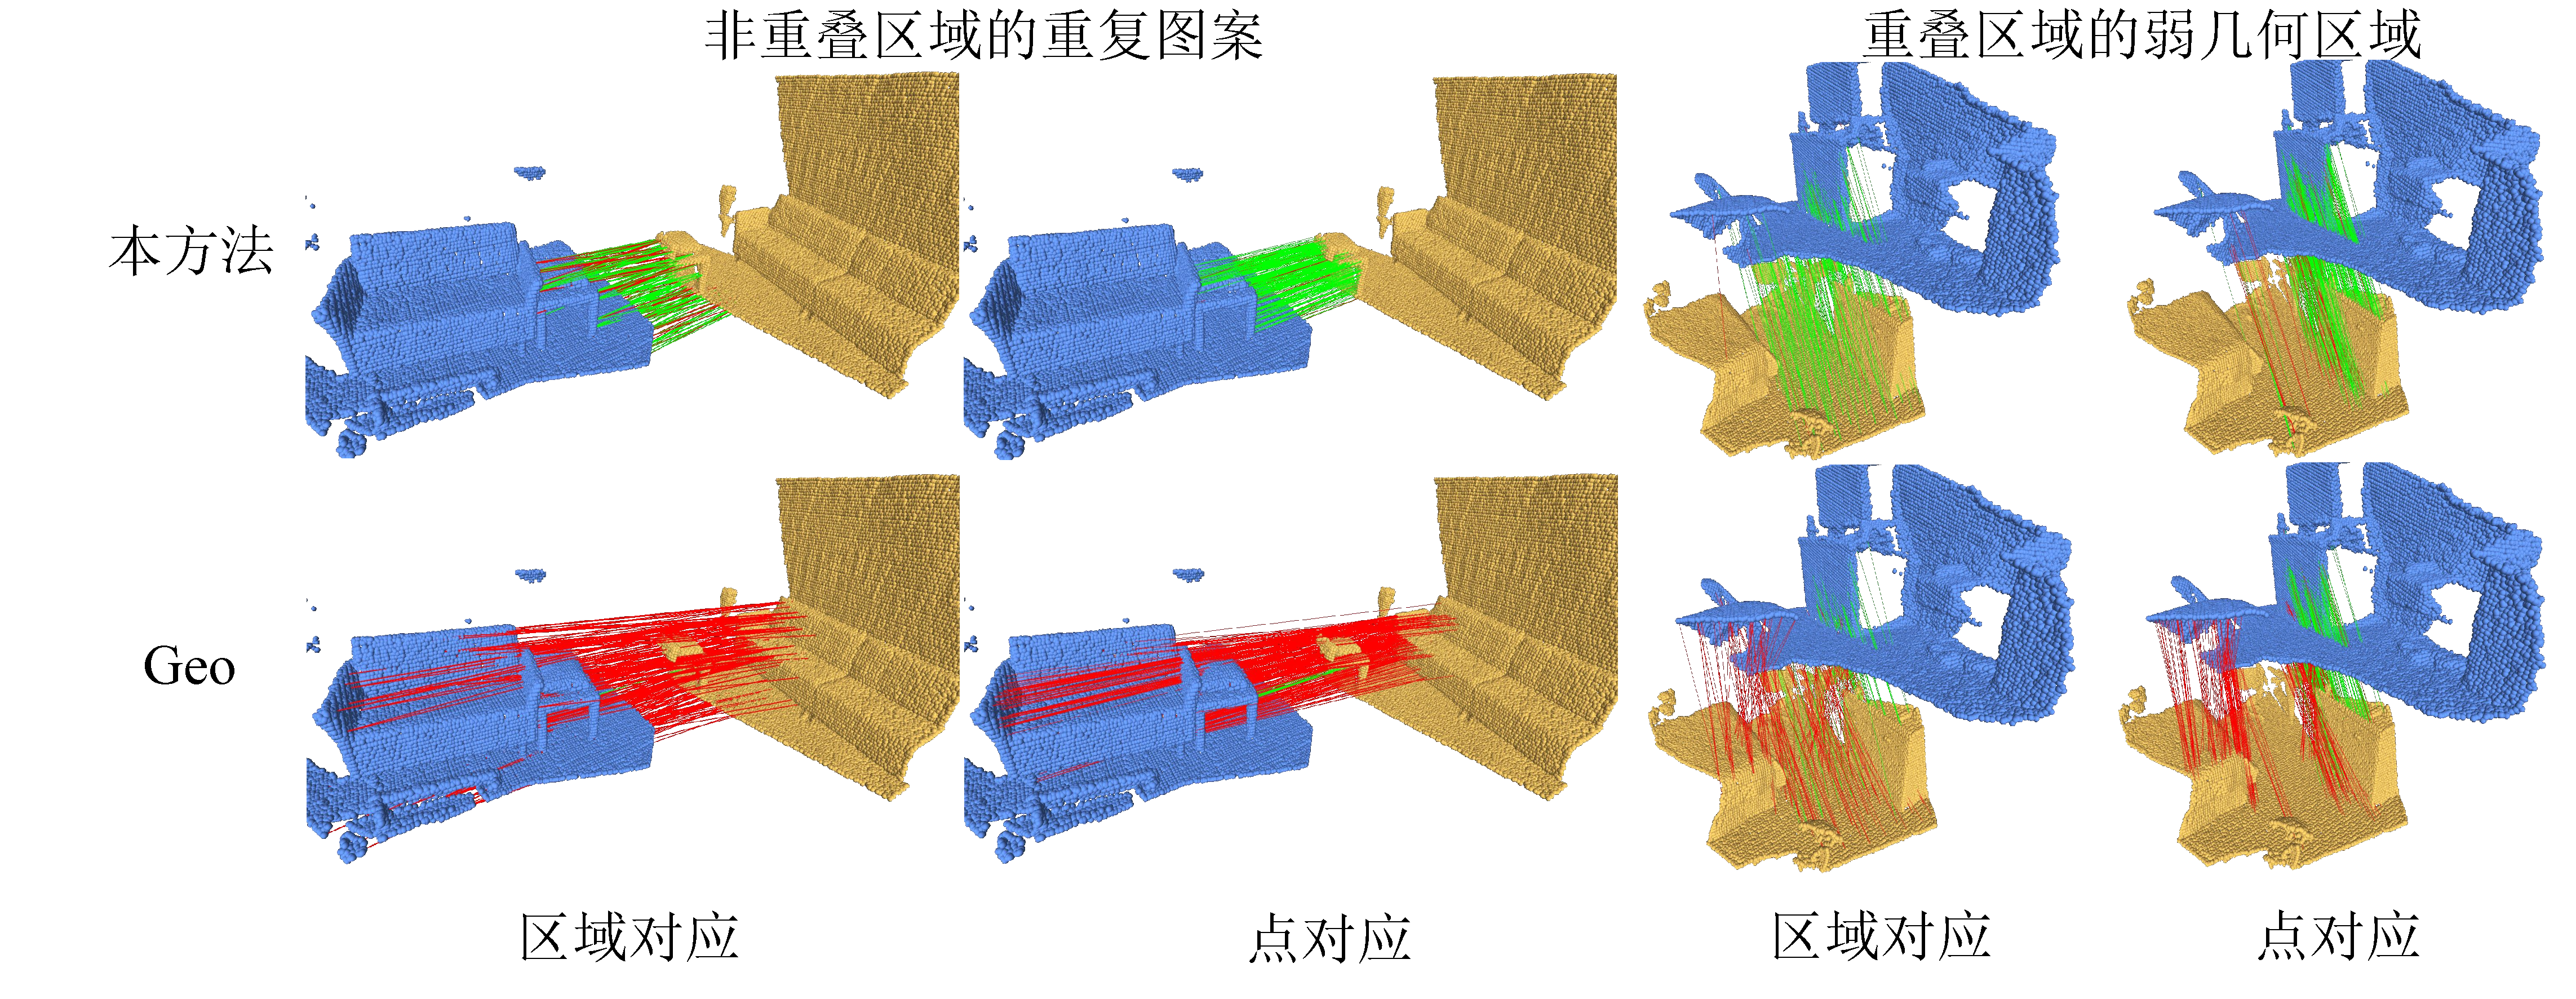
\includegraphics[width = \textwidth]{my/figure/3-1.pdf}
        % \captionsetup{margin = {1.6cm,1.6cm}}
        \bicaption[\xiaosi 第三章方法和Geo在具有几何挑战性的情况下的对比]{\wuhao 本方法和Geo在具有几何挑战性的情况下的对比。}{\wuhao Comparison of our method and Geo in geometrically challenging situations. }
        \label{fig:example}
    \end{figure}
    \vspace{-0.35cm}

    因此,在本章中,提出了一种鲁棒点云配准方法。一组包含相对丰富的判别几何信息的超点对应被定位为显著锚点对应,显著锚点对应由锚点定位模块产生。由于正确的超点对应与这组显著锚点对应存在几何空间一致性,因此将超点与显著锚点之间的几何进行嵌入可以有效地剔除异常值。又由于相似非重叠区域超点以及弱几何区域超点相对于这组锚点的几何位置不同,因而其几何特征也会存在差异,因此将锚点与超点的几何特征进行嵌入能够有效增加上述两种情况超点间的差异性,使得模型能够在几何挑战较大的区域获得准确的点对应。该方法不仅能够提高点云配准的准确性,还能够有效处理异常值和几何挑战较大的情况,具有广泛的应用前景。

    具体来说,本章节首先设计了一个锚点定位模块,利用非极大值抑制法来获取源点云和目标点云上分布稀疏且保持一定几何结构的锚点对应。通过显著锚点,本方法提出了一种选择性几何嵌入模块,增强了超点特征间的差异性,以实现精确的超点匹配。本研究利用注意力机制,有选择地嵌入锚点的几何信息,而不是聚集周围超点的所有几何信息。利用交叉注意力机制,将锚点-超点的距离和角度嵌等选择性几何信息入。为了获取最有效的锚点和显著特征,迭代更新锚点的位置和超点特征,这对于获得精确的超点对应关系起着至关重要的作用。最后,利用姿态估计器通过点的对应关系来生成最终的变换矩阵。\par
    (1)提出了一个健壮的点云配准框架,通过嵌入显著性锚点的几何结构,能够实现具有弱几何结构和重复图案的点云配准的最先进性能。
    (2)设计了一种选择性几何结构嵌入方法,通过在超点和显著锚点之间嵌入几何信息来增强超点特征的区别。
    (3) 提出了一种锚点定位和更新方法,以获得在源点云和目标点云的重叠区域中分布稀疏且包含丰富的判别几何信息的最有效的锚点。

    \section{基于显著锚点几何嵌入的点云配准方法}
    \subsection{问题陈述}
    给定来自不同视角的且部分重叠的源点云$\mathcal{P}=\{{\mathbf{p}_i} \in \mathbb{R}^{3} \mid i=1,..,N\}$和目标点云$\mathcal{Q}=\{{\mathbf{q}_j} \in \mathbb{R}^{3} \mid j =1,\dots,M\}$,点云配准的目标是求解变换矩阵$\mathbf{Trans}$使得两点云对齐。$\mathbf{Trans}$由旋转矩阵$\mathbf{R}$和平移向量$\mathbf{t}$组成,数学描述由公式(3-1)表示:
    \begin{equation}
        \mathrm{arg}\underset{\mathbf{R}, \mathbf{t}}{\min} \sum_{(\mathbf{p}_i, \mathbf{q}_j) \in \mathcal{C}} 
        {\left\|{\mathbf{q}_j-(\mathbf{R} \cdot \mathbf{p}_i+\mathbf{t})}\right\|_{2}^{2}}
    \end{equation}
    式中,$(\mathbf{p}_i, \mathbf{q}_j)$属于集合$\mathcal{C}$,表示源点云的$\mathbf{p}_i$点和目标点云的$\mathbf{q}_j$是一对对应点。如第二章所述,求解变换矩阵的问题转换为了寻找对应关系集合$\mathcal{C}$的问题。

    \subsection{方法概述}
    如图\ref{fig:framework}所示,在使用共享骨干网络提取点云特征后,本方法首先使用所提出的锚点定位模块在源点云和目标点云中定位初始锚点对应关系。在选定锚点的基础上,结合锚点的几何特征,提出了选择性几何嵌入模块,增强了超点特征的区分性。为了获得最显著的锚点和差异性的超点特征,提出了一种基于迭代优化的显著锚点更新(IOSAU)方法,以迭代方式更新锚点位置和超点特征。通过迭代增强特征差异性,可以实现精确的超点匹配。然后在每个超点内获得可靠的点对点的对应关系。最后,利用姿态估计器获得变换矩阵并进行精确配准。

    \vspace{-0.1cm}
    \begin{figure}[h]
        \centering
        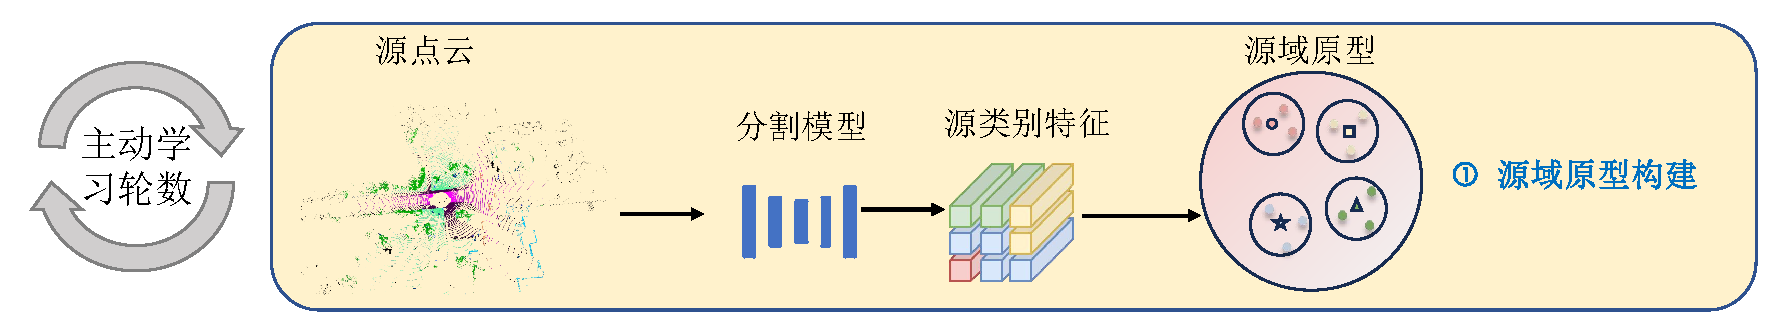
\includegraphics[width = \textwidth]{my/figure/3-2.pdf}
        \bicaption[\xiaosi 第三章点云配准方法概述]{\wuhao 本点云配准方法概述}{\wuhao Overview of the proposed registration method}\label{fig:framework}
    \end{figure}
    \vspace{-0.35cm}

    \subsection{锚点定位模块}
    本研究首先将源点云$\mathcal{P}$和目标点云$\mathcal{Q}$送入共享骨干网络KPConv中。在这个网络中原始点云将被下采样为超点并提取特征,本文用符号$\mathcal{\hat{P}} = \{\mathbf{\hat{p}}_i\}_{i=1}^{|\mathcal{\hat{P}}| }$和$\mathcal{\hat{Q}} = \{\mathbf{\hat{q}}_j\}_{j=1}^{|\mathcal{\hat{Q}}| }$分别表示源点云和目标点云的超点,用符号$\mathbf{F}^{\hat{\mathcal{P}}} \in \mathbb{R}^{\left|\mathcal{\hat{P}}\right| \times \hat{d}}$和$\mathbf{F}^{\hat{\mathcal{Q}}} \in \mathbb{R}^{\left|\mathcal{\hat{Q}}\right| \times \hat{d}}$分别表示这些超点的特征。下采样和特征提取过程可以表述为:
    $\left(\mathbb{R}^{\left|\mathcal{P}\right|\times 3},
    \mathbb{R}^{\left|\mathcal{Q}\right|\times 3}\right) 
    \rightarrow 
    \left(\mathbb{R}^{\left|\hat{\mathcal{P}}\right| \times \hat{d}}, 
    \mathbb{R}^{\left|\hat{\mathcal{Q}}\right| \times \hat{d}}\right)$,其中$ \hat{d}$表示超点特征的通道数。\par

    \vspace{-0.1cm}
    \begin{algorithm}[h]
        \caption{锚点定位}
        \label{alg:anchor_location}
        \LinesNumbered 
        \KwIn{抑制半径$r_{nms}$, 相似矩阵$\mathbf{S}$, 锚点个数$K$}
        \KwOut{$\mathcal{\hat{C}} = \{(\mathbf{\hat{a}}_k,\mathbf{\hat{b}}_k) \mid k=1,\dots,K\}$。其中$\mathbf{\hat{a}}_k$、$\mathbf{\hat{b}}_k$分别表示第$k$个锚点对应在源点云和目标点云中的坐标。}
    
        $\mathcal{\hat{C}} = \phi$ \\
        \While{$|\mathcal{\hat{C}}|<K$}{
            $S_{i,j}=max(\mathbf{S})$; \\
            $\mathcal{\hat{C}} = \mathcal{\hat{C}} \cup (\mathbf{\hat{p}}_{i}, \mathbf{\hat{q}}_{j})$; \\
                \For{$x \in \{1,2,...,row(\mathbf{S})\}$}{
                \If{$||\mathbf{\hat{p}}_{i}-\mathbf{\hat{p}}_{x}||_2<r$}{
                    remove($\mathbf{S}_{x,-}$)
                }
            }
                \For{$y \in \{1,2,..., col(\mathbf{S})\}$}{
                \If{$||\mathbf{\hat{q}}_{j}-\mathbf{\hat{q}}_{y}||_2<r$}{
                    remove($\mathbf{S}_{-,y}$)
                }
            }
        }
    \end{algorithm}
    \vspace{-0.35cm}

    在获取超点后,本方法再定位源点云和目标点云中保持一定几何结构的的锚点对应。一旦得到可靠的锚点对应,就可以将它们作为参考点,将锚点与超点之间的几何结构信息嵌入到每个超点特征中。这样就可以消除特征相似导致的错误超点匹配。因此,在锚点定位模块中,本模块的目标是获取那些具有判别特征的超点对应作为显著锚点对应。\par

    给定源点云和目标点云的超点特征$\mathbf{F}^{\hat{\mathcal{P}}}$和$\mathbf{F}^{\hat{\mathcal{Q}}}$,初始锚点对应可以选择在相似矩阵$\mathbf{S}$中具有较高置信度的超点对应。如图\ref{fig:framework}所示,为了获得分布稀疏的保持一定几何结构的锚点对应,本方法放弃了传统的Top-K选择方法,即连续选择几个最高置信度的超点匹配,避免了所选锚点对应关系位置集中。原因是因为当这组锚点存在聚集情况时,在后续几何嵌入过程中聚集的多个锚点就会退化为一个锚点。对于一个锚点而言,无论是角度还是距离,不同超点与它之间的结构差异性就会丢失。因此,本模块采用非最大值抑制\upcite{NMS}(Non-Maximum Suppression,NMS)来保证所选锚点对应的空间均匀性和稀疏性。首先利用$\mathbf{F}^{\hat{\mathcal{P}}}$和$\mathbf{F}^{\hat{\mathcal{Q}}}$计算源点云和目标点云的超点之间的相似分数矩阵,并从置信度最高到最低进行排序。非最大抑制应用于每个超点周围的固定半径$r_{nms}$。在选择最高置信度的超点后,去除所有在$r_{nms}$的欧氏距离内的对应关系。在剩余的超点中,本模块选择置信度最高的对应作为第二锚点对应,并删除位于$r_{nms}$半径内的对应。重复这个过程,直到本模块获得$K$个初始锚对应,定义如公式(3-2)所示:
    \begin{equation}
        \hat{\mathcal{C}}=\{(\mathbf{\hat{a}}_k,\mathbf{\hat{b}}_k) \mid k =1,\dots,\mathrm{K}\}
    \end{equation}
    式中,$\mathbf{\hat{a}}_k$、$\mathbf{\hat{b}}_k$分别表示第$k$个锚点对应在源点云和目标点云中的坐标。算法\ref{alg:anchor_location}描述了锚点定位的整个过程。

    \subsection{选择性几何嵌入模块}
    在提出的选择性几何嵌入模块中,融合了锚点和超点之间的几何信息。每个点云内部的超点距离通过自注意机制嵌入到超点特征中。在两个点云信息交流过程中,本模块将超点与所有锚点之间的角度和距离进行编码,并与超点的特征进行融合。本方法没有直接将一个点云上的所有超点信息聚合到另一个点云上,而是有选择地嵌入相应锚点的几何信息,进一步增强了超点特征的显著性。将锚点的几何形状嵌入有以下几个优点:(1)在源点云和目标点云只有部分重叠的情况下,直接交换两个点云的所有信息会不可避免地会引入噪声和扰动;(2)有选择地嵌入稀疏和正确的锚点几何,可以避免弱几何区域的对称、上下和前后翻转问题。\par
    本模块为每个点云构造锚点与超点间的距离和角度。当锚点匹配时,正确对应的超点具有一致的锚点距离和角度。为此,本模块利用交叉注意机制将这种几何一致性合并到超点特征中,从而实现点云几何信息的交换。通过这种方式,本模块的选择性几何嵌入模块能够帮助匹配更精确的超点对应。\par

    \subsubsection{内部结构嵌入}
    点云内部结构包含上下文全局信息,有利于增加超点特征间的区分度。在自注意机制中,本模块明确地将超点间的距离信息嵌入到点云特征中。下面本文将以以源点云为例详细说明内部结构嵌入的整个过程。
    给定源点云中的一个超点$\mathbf{\hat{p}}_{i}$,本模块首先计算超点$\mathbf{\hat{p}}_{i}$与其他任意超点$\mathbf{\hat{p}}_{i}$之间的距离,并根据超参数$\sigma_{d}$调节二者的距离灵敏度,随后利用正弦函数将$\mathbf{\hat{p}}_{i}$与$\mathbf{\hat{p}}_{i}$的距离这一标量映射到高维空间,具体流程由公式(3-3)表示:
    \begin{equation}
        \centering
            \mathbf{E}_{sa}^{\mathcal{\hat{P}}_{(i,j)}} = f(d(\mathbf{\hat{p}}_{i},\mathbf{\hat{p}}_{j})/\sigma_{d})
    \end{equation}
    式中,$d(\mathbf{\hat{p}}_{i},\mathbf{\hat{p}}_{j})=\left\|{\mathbf{\hat{p}}_{i}-\mathbf{\hat{p}}_{j}}\right\|_{2}^{2}$表示超点$\mathbf{\hat{p}}_{i}$和$\mathbf{\hat{p}}_{j}$之间的距离;$\sigma_{d}$是调节距离灵敏度的系数,一般设置在$0.1\sim 0.5$之间;$f(\cdot)$表示一个正弦函数,它将标量映射到高维特征。

    给定超点特征$\mathbf{F}^{\mathcal{\hat{P}}}$和距离编码$\mathbf{E}_{sa}^{\mathcal{\hat{P}}}$,利用自注意力机制将超点特征与超点距离编码进行融合。
    利用三个可学习矩阵$\mathbf{W}_{q}$,$\mathbf{W}_{k}$和$\mathbf{W}_{v}$分别将$\mathbf{F}^{\mathcal{\hat{P}}}$映射为$\mathbf{F}_{q}^{\mathcal{\hat{P}}}$、$\mathbf{F}_{k}^{\mathcal{\hat{P}}}$和$\mathbf{F}_{v}^{\mathcal{\hat{P}}}$。
    $\mathbf{W}_{g}$用来将$\mathbf{E}_{sa}^{\mathcal{\hat{P}}}$映射到$\mathbf{E}_{g}^{\mathcal{\hat{P}}}$。然后利用$\mathbf{F}_{q}^{\mathcal{\hat{P}}}$、$\mathbf{F}_{k}^{\mathcal{\hat{P}}}$、$\mathbf{E}_{g}^{\mathcal{\hat{P}}}$计算相似度矩阵$\mathbf{Score}$,其中矩阵每一行每一列的值由公式(3-4)计算:
    \begin{equation}
        \centering
        \mathbf{Score}_{(i, j)}= 
        \frac{
        \mathbf{F}_{q}^{\mathcal{\hat{P}}_{i}} \cdot (\mathbf{F}_{k}^{\mathcal{\hat{P}}_{j}} + \mathbf{E}_{g}^{\mathcal{\hat{P}}_{(i, j)}})^\mathrm{T}
        }{\sqrt{\hat{d}}}
    \end{equation}
    融合点云自身结构信息后的超点特征$\mathbf{F}^{\mathcal{\hat{P}}}$可由公式(3-5)计算得到:
    \begin{equation}
        \centering
        \mathbf{F}^{\mathcal{\hat{P}}} =softmax(\mathbf{Score}) \cdot \mathbf{F}_{v}^{\mathcal{\hat{P}}}
    \end{equation}\par

    \subsubsection{外部结构嵌入}
    两点云之间的信息交流在点云配准问题中起着至关重要的作用,特别是在低重叠的情况下。即使通过自我注意力机制嵌入了自身的几何图形,由于源点云和目标点云中普遍存在重复的图案,仍然存在区域特征相似的情况。对于这些超点,相似的特征会导致源点云和目标点云之间的不匹配。因此,需要在目标点云和源点云之间通过显著锚点对应进行信息交换。与Geo方法不加区别地使用交叉注意力融合另一帧点云特征的方式不同,本模块采用一种选择性几何嵌入方法,构建锚点和超点之间的结构编码,然后将源点云和目标点云信息进行交流。其过程如图\ref{fig:cross_attention}所示。源点云和目标点云的超点的特征和几何结构使用交叉注意机制显式地融合。\par

    \vspace{-0.1cm}
    \begin{figure}[htp]
        \centering
        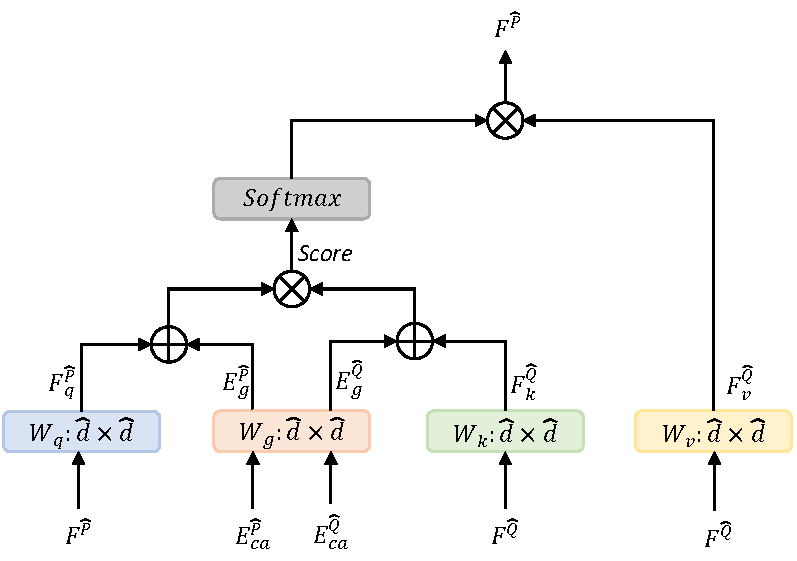
\includegraphics[width = 8.5cm]{my/figure/3-3.pdf}
        \bicaption[\xiaosi 交叉注意力的计算图]{\wuhao 交叉注意的计算图}{\wuhao The computation graph of cross-attention}
        \label{fig:cross_attention}
    \end{figure}
    \vspace{-0.35cm}

    对于源点云中的某个超点$\hat{\mathbf{p}}_{n}$,$\{\hat{\mathbf{a}}_i\}_{i=1}^K$表示为锚点集合,本模块用公式(3-6)计算上超点与第$i$个锚点之间的距离:
    \begin{equation}
        \rho_{i} = d(\hat{\mathbf{p}}_{n},\hat{\mathbf{a}}_i)
    \end{equation}
    然后同内部结构嵌入一致,使用$f(\cdot)$函数将锚点与超点的距离映射到高维特征。然后根据锚点对应得分进行加权求和,形成超点距离编码如公式(3-7)所示:
    \begin{equation}
        \mathbf{Ed}_{ca}^{\mathcal{\hat{P}}_{n}}=  \sum_{i=1}^{K} {f(\rho_{i})/\sigma_{d}}
    \end{equation}
    式中,$\mathbf{Ed}_{ca}^{\mathcal{\hat{P}}_{n}}$是锚点-超点距离嵌入;$K$表示锚点数量;$\sigma_{d}$是用于调节距离灵敏度的参数。除了距离嵌入,超点与锚点之间的角度也被融合到特征中。如图\ref{fig:embedding}所示,本方法以$\hat{\mathbf{p}}_n$为顶点。顶点和两个锚点组成一个夹角,定义为公式(3-8):
    \begin{equation}
        \centering
        \theta_k(\mathbf{\hat{p}}_n, \mathbf{\hat{a}}_l, \mathbf{\hat{a}}_s)= deg(\mathbf{\hat{a}}_l-\mathbf{\hat{p}}_n,\mathbf{\hat{a}}_s - \mathbf{\hat{p}}_n)
    \end{equation}
    式中,$\theta$表示锚点与超点之间角度;$\mathbf{\hat{a}}_l$表示源点云中的第$l$个锚点;$\mathbf{\hat{a}}_s$表示源点云中的第$s$个锚点;$deg(\cdot)$表示计算角度的度函数。在获得锚点与超点的夹角后,本模块使用正弦函数$f(\cdot)$将其映射到高维特征。然后利用置信度加权和得到超点的角度编码,如公式(3-9)所示:
    \begin{equation}
        \mathbf{Ea}_{ca}^{\mathcal{\hat{P}}_{n}} = \sum_{k = 1}^{C_K^2} f(\theta_k(\mathbf{\hat{p}}_{n}, \mathbf{\hat{a}}_l, \mathbf{\hat{a}}_s)/\sigma_\theta)
    \end{equation}
    式中,$K$为锚点的个数;$C_K^2$为组合的个数;$\sigma_\theta$是调节角度灵敏度的系数。然后,将超点距离编码$\mathbf{Ed}_{ca}^{\mathcal{\hat{P}}_n}$与超点角度$\mathbf{Ea}_{ca}^{\mathcal{\hat{P}}_n}$相加,利用公式(3-10)得到最终的超点几何编码:
    \begin{equation}
        \mathbf{E}_{ca}^{\mathcal{\hat{P}}_{n}} =  \mathbf{Ed}_{ca}^{\mathcal{\hat{P}}_{n}} + \mathbf{Ea}_{ca}^{\mathcal{\hat{P}}_{n}}
    \end{equation}

    上述锚点与超点间的几何结构嵌入过程如图\ref{fig:embedding}所示,首先计算出锚点与超点之间的距离和角度,并进行编码,随后将角度和距离编码进行信息合并,形成最终的几何编码。对于目标点云中的超点$\mathbf{\hat{q}}_m$,可以用同样的方法得到几何编码,记为$\mathbf{E}_{ca}^{\mathcal{\hat{Q}}_m}$。\par

    利用KPConv提取的超点特征$\mathbf{F}^{\mathcal{\hat{P}}_n}$和$\mathbf{F}^{\mathcal{\hat{Q}}_m}$,以及在源点云和目标点云中几何编码$\mathbf{E}_{ca}^{\mathcal{\hat{P}}_{n}}$和$\mathbf{E}_{ca}^{\mathcal{\hat{Q}}_{m}}$,通过交叉注意力技术进行融合。
    本方法利用可学习的矩阵$\mathbf{W}_q$将$\mathbf{F}^{\mathcal{\hat{P}}_n}$映射到$\mathbf{F}_{q}^{\mathcal{\hat{P}}_n}$,利用可学习的矩阵$\mathbf{W}_k$和$\mathbf{W}_v$将$\mathbf{F}^{\mathcal{\hat{Q}}_m}$映射到$\mathbf{F}_{k}^{\mathcal{\hat{Q}}_m}$和$\mathbf{F}_{v}^{\mathcal{\hat{Q}}_m}$,利用可学习的矩阵$\mathbf{W}_g$将$\mathbf{E}_{ca}^{\mathcal{\hat{P}}_{n}}$和$\mathbf{E}_{ca}^{\mathcal{\hat{Q}}_{m}}$映射到$\mathbf{E}_{g}^{\mathcal{\hat{P}}_{n}}$和$\mathbf{E}_{g}^{\mathcal{\hat{Q}}_{m}}$。然后由公式(3-11)计算系数矩阵$\mathbf{Score}^{\mathcal{\hat{Q}}\to\mathcal{\hat{P}}}$:
    \begin{equation}
        \mathbf{Score}_{(n, m)}^{\hat{\mathcal{Q}}\to\hat{\mathcal{P}}}=
        \frac{
        {(\mathbf{F}_q^{\mathcal{\hat{P}}_n}+\mathbf{E}_g^{\mathbf{\hat{P}}_n})}\cdot
        {(\mathbf{F}_k^{\mathcal{\hat{Q}}_m}+\mathbf{E}_g^{\mathbf{\hat{Q}}_m})}^\mathrm{T}
        }{\sqrt{\hat{d}}}
    \end{equation}

    在使用交叉注意力机制进行信息交流后,可以使用公式(3-12)计算源点云$\bar{\mathbf{F}}^{\mathcal{\hat{P}}_n}$的超点特征:
    \begin{equation}
        \begin{aligned}  
        \mathbf{\bar{F}}^{\mathcal{\hat{P}}_n} = 
        softmax(\mathbf{Score}_{(n, m)}^{\mathcal{\hat{Q}}\to\mathcal{\hat{P}}})
        \cdot \mathbf{F}_v^{\mathcal{\hat{Q}}_m}
        \end{aligned}
    \end{equation}
    给定目标点云中的一个超点$\mathbf{\hat{q}}_m$,本方法可以按照上述交叉注意过程,得到目标点云到源点云的系数矩阵$\mathbf{Score}_{(n, m)}^{\mathcal{\hat{P}}\to\mathcal{\hat{Q}}}$,并根据$\mathbf{Score}_{(n, m)}^{\mathcal{\hat{P}}\to\mathcal{\hat{Q}}}$更新目标点云超点特征$\mathbf{\bar{F}}^{\mathcal{\hat{Q}}_m}$。通过选择性几何嵌入,显著锚点的几何一致性融合到点云特征中。这样可以对几何形状较弱、图案重复的区域特征进行区分,提高匹配精度。

    \vspace{-0.1cm}
    \begin{figure}[h]
        \centering
        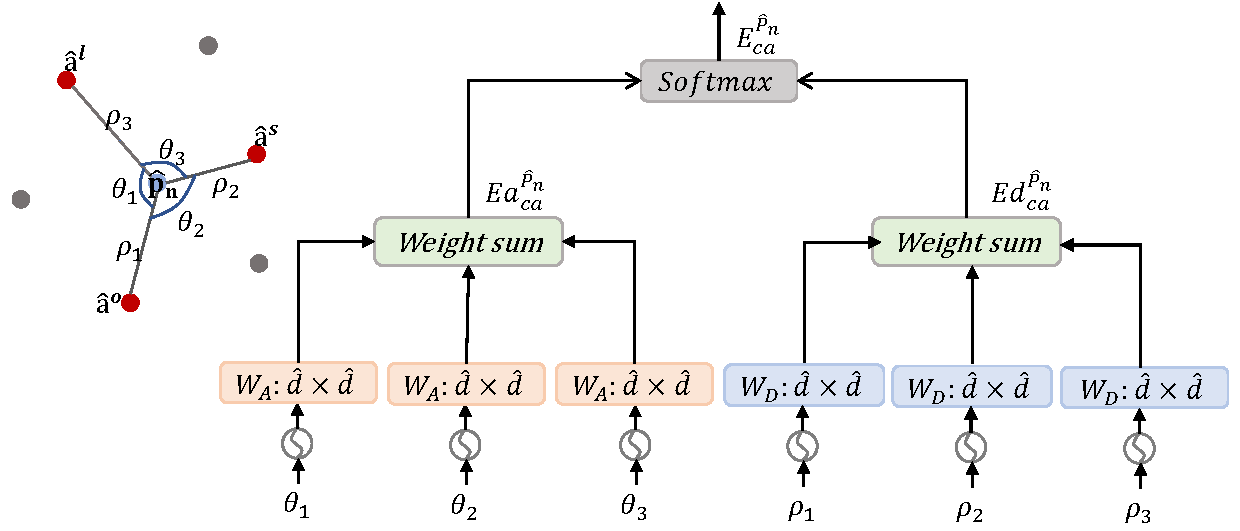
\includegraphics[width = 12cm]{my/figure/3-4.pdf}
        \bicaption[\xiaosi 几何结构嵌入计算图]{\wuhao 几何结构嵌入计算图}{\wuhao The computation graph of geometric structure embedding}
        \label{fig:embedding}
    \end{figure}
    \vspace{-0.35cm}

    \subsection{基于迭代优化的显著锚点更新}
    如前所述,差异性特征有利于定位最显著的锚点,嵌入锚点的几何编码能够使超点特征更具区分度。然而,在初始阶段,神经网络训练不够好,初始锚点对应关系不够准确,分布不够稀疏,导致几何编码不能充分捕获结构信息。
    为了获取精确的几何编码,本章节提出了迭代更新锚点和超点对应关系的方法。真实的超点匹配可以促进获得显著锚点,进而有利于获得精确的超点对应。在迭代过程中,初始错误选择的锚对应关系由于不一致而对特征的不利影响较小。相反,具有一致性的正确锚对应在多次迭代中逐渐增强。

    给定点云的超点$\hat{\mathcal{P}}$、$\hat{\mathcal{Q}}$和对应的超点特征$\mathbf{F}^{\hat{\mathcal{P}}}$、$\mathbf{F}^{\hat{\mathcal{Q}}}$,将其输入到锚点定位模块中获取初始锚点对应关系$\hat{\mathcal{C}}$。通过选择性几何嵌入模块,利用自注意机制和交叉注意机制嵌入初始锚点对应和超点的几何,获得增强的超点特征$\bar{\mathbf{F}}^{\hat{\mathcal{P}}}$和$\bar{\mathbf{F}}^{\hat{\mathcal{Q}}}$。为了更新锚点位置,将增强的特征点坐标重新输入到锚点位置和选择性几何嵌入模块中。

    在获得最终的超点特征$\bar{\mathbf{F}}^{\hat{\mathcal{P}}}$和$\bar{\mathbf{F}}^{\hat{\mathcal{Q}}}$之后,本模块首先将它们归一化,并计算相似矩阵$\hat{\mathbf{S}} = \bar{\mathbf{F}}^{\hat{\mathcal{P}}} (\bar{\mathbf{F}}^{\hat{\mathcal{Q}}})^T /\sqrt{\hat{d}}$。值得注意的是,有些超点不在重叠区域因此没有对应点,所以本模块在矩阵$\hat{\mathbf{S}}$中添加一行和一列作为松弛项。将没有对应关系的超点与松弛项进行对应,以保持正确的对应关系。然后使用Sinkhorn算法对整个矩阵进行优化。最后选取得分最高的$K_s$个对应点作为最终的超点匹配结果,其定义如公式(3-13)所示:
    \begin{equation}
        \begin{aligned}
        \mathcal{\hat{SC}}=
        \left\{
        (\mathbf{\hat{p}}_{x_{i}}, \mathbf{\hat{q}}_{y_{i}}) \mid
        \mathbf{\hat{S}}(x_{i}, y_{i}) \in \operatorname{topk}(\mathbf{\hat{S}})
        \right\}
        \end{aligned}
    \end{equation}
    式中,$\operatorname{topk}(\hat{\mathbf{S}})$返回矩阵$\hat{\mathbf{S}}$中最大$K_s$项的对应超点;$x_{i}$和 $y_{i}$分别表示源点云和目标点云中第$i$对超点对应的下标。

    \subsection{点匹配模块}
    在得到超点对应$\mathcal{\hat{SC}}$后,利用骨干网络的解码器模块对超点进行上采样并提取点特征。本方法先根据空间中的位置关系将每个点划分到最近的超点中,每个超点将有一个内部的点集合。然后根据超点对应寻找内部的点对应。不失一般性,对于任一超点对应$\mathcal{\hat{SC}}_i=(\mathbf{\hat{p}}_{x_{i}}, \mathbf{\hat{q}}_{y_{i}})$, $\mathbf{\hat{p}}_{x_{i}}$的内部点集合记为$\mathcal{G}_{x_i}^{\mathcal{P}}$, $\mathbf{\hat{p}}_{x_{i}}$的内部点集合记为$\mathcal{G}_{y_i}^{\mathcal{Q}}$。接着本文计算集合$\mathcal{G}_{x_i}^{\mathcal{P}}$中每个点与集合$\mathcal{G}_{y_i}^{\mathcal{Q}}$中每个点的相似度,得到相似度矩阵$\mathbf{S}_i$。并选取出$\mathbf{S}_i$中$K_p$个最高分项作为点对应,其数学表达如公式(3-14):
    \begin{equation}
        \begin{aligned}
        \mathcal{PC}_i=
        \left\{
        (\mathcal{G}_{x_i}^{\mathcal{P}}(n), \mathcal{G}_{y_i}^{\mathcal{Q}}(m)) \mid
        \mathbf{S}_i(n, m) \in \operatorname{topk}({\mathbf{S}_i})
        \right\}
        \end{aligned}
    \end{equation}
    随后可以得到最终的点对应集合$\mathcal{PC} = \bigcup_{i=1}^{K_s} \mathcal{PC}_i$

    \subsection{变换矩阵估计}
    传统的点云描述符通常不能捕获足够明显的特征。因此,得到的点对应往往存在大量异常值。为了得到精确的变换,RANSAC作为一种鲁棒估计器,从具有高离群率的点对应集中计算姿态。然而,RANSAC收敛速度慢。为了实现准确高效的变换估计,本方法首先根据所提出的几何嵌入特征获取高置信区域匹配,然后在区域匹配内捕获目标点云和源点云的点对应关系。因此,在不像RANSAC那样去除异常值的情况下,本方法无需迭代就可以估计变换矩阵。对于第$i$个超点对应的旋转$\mathbf{R'}_i$和平移$\mathbf{t'}_i$可以利用公式(3-15)计算:
    \begin{equation}
        \begin{aligned}
        \mathbf{R'}_i, \mathbf{t'}_i=
        \mathrm{arg}\min_{\mathbf{R},\mathbf{t}} 
        \sum_{(\mathbf{p}_{x_j},\mathbf{q}_{y_j}) \in \mathcal{PC}_i}
        w_{j}
        \left\|
        \mathbf{R}\cdot\mathbf{p}_{x_j}+\mathbf{t}-\mathbf{q}_{y_j}
        \right\|_{2}^{2}
        \end{aligned}
    \end{equation}\par

    对于任一的$\mathbf{R'}_i$,$\mathbf{t'}_i$可以通过SVD得到代数解。在得到$K_s$个局部旋转矩阵$\mathbf{R'}$和平移向量$\mathbf{t'}$后,本文从中选取出最优的$\mathbf{R'}_i$,$\mathbf{t'}_i$作为最终配准结构。本方法将所有$\mathbf{R'}_i, \mathbf{t'}_i$应用到最终的点对应集合$\mathcal{PC}$,并计算所有点对应的距离和作为误差判断。最终的变换估计由公式(3-16)表示:
    \begin{equation}
        \begin{aligned}
        \mathbf{R}, \mathbf{t}=
        \mathrm{arg}\min_{\mathbf{R'}_i,\mathbf{t'}_i} 
        \sum_{(\mathbf{p}_{x_j},\mathbf{q}_{y_j}) \in \mathcal{PC}}
        \left\|
            \mathbf{R'}_i\cdot\mathbf{p}_{x_j}+\mathbf{t'}_i-\mathbf{q}_{y_j}
        \right\|_{2}^{2}
        \end{aligned}
    \end{equation}

    \subsection{损失函数}
    训练损失函数$\mathcal{L}$由超点对应损失$\mathcal{L}_c$和点对应损失$\mathcal{L}_f$两部分组成。\par
    \subsubsection{超点对应损失函数}
    本文采用一个变形圆损失来监督超点匹配。首先,如果源点云$\mathcal{P}$中的一个超点与目标点云$\mathcal{Q}$中的一个超点有至少10\%的重叠,将认为这对超点对应是正样本。否则,超点对应被视为负样本。其次,选取$\mathcal{P}$中所有至少有一个正样本的超点,构成基本集$\mathcal{P}_p$。对于每个超点$\hat{\mathbf{p}}_i \in  \mathcal{P}_p$, $\mathcal{Q}$中的正超点构成$\varepsilon_p^i$集,负超点构成$\varepsilon_n^i$集。最后定义$\mathcal{P}$上的变形圆损失如公式(3-16)所示:
    \begin{equation}
        \mathcal{L}_{c}^{\mathcal{P}}=
        \frac{1}{|\mathcal{P}_p|}
        \sum_{\hat{\mathbf{p}}_i \in \mathcal{P}_p} 
        \log[1+\sum_{\hat{\mathbf{q}}_j \in \varepsilon_{p}^{i}}e^{\lambda_{i}^{j} \beta_{p}^{i, j}\left(d_{i}^{j}-\Delta_{p}\right)}
        \cdot \sum_{\hat{\mathbf{q}}_k \in \varepsilon_{n}^{i}}e^{\beta_{n}^{i, k}\left(\Delta_{n}-d_{i}^{k}\right)}]
    \end{equation}
    式中,$d_i^j$表示特征空间中的距离;若超点$\hat{\mathbf{p}}_i$与$\hat{\mathbf{q}}_j$的重叠率$o_i^j$,那么$\lambda_{i}^{j}=\sqrt{o_i^j}$。正裕量$\Delta_{p}$和负裕量$\Delta_{n}$分别设为$0.1$和$1.4$。同时,对每个样品分别计算其正权$\beta_{p}^{i, j}= \gamma \left(d_{i}^{j}-\Delta_{p}\right)$和负权$\beta_{n}^{i, k} = \gamma \left(\Delta_{n}-d_{i}^{k}\right)$。

    \subsubsection{点对应损失函数}
    对于点匹配,本文使用负对数似然函数\upcite{Superglue}来监督每个超点对应的点匹配分数矩阵。在训练阶段,本文选择$N_g$个真实超点匹配,计算对应区域中的真实点对应集$\mathcal{M}_{i}$。然后将两个区域中的未匹配点划分为$\mathcal{I}_{i}$和$\mathcal{J}_{i}$两组。所选第$i$个超点对应区域内的点对应的损失函数定义为公式(3-17):
    \begin{equation}
        \mathcal{L}_{f}^i=
        -\sum_{(x, y) \in \mathcal{M}_{i}} \log \mathbf{S}_i(x,y)
        -\sum_{x \in \mathcal{I}_{i}} \log \mathbf{S}_i(x, m_{i}+1)
        -\sum_{y \in \mathcal{J}_{i}} \log \mathbf{S}_i(n_{i}+1, y)
    \end{equation}
    式中,$\mathbf{S}_i(x,y)$表示第$i$个超点对应内部区域的点对应系数矩阵$\mathbf{S}_i$第$x$行第$y$列的值。
    最终的精细的点对应损失函数是选取$N_g$超点的点对应损失的平均值,定义为公式(3-18):
    \begin{equation}
        \mathcal{L}_{f}=\frac{1}{N_g}\sum_{i=1}^{N_g}\mathcal{L}_{f}^i
    \end{equation}

    \section{实验分析}
    在本节中进行了大量的实验来评估本方法研究的有效性。实验实施细节将在第3.3.1节中描述。在3.3.2和3.3.3节中,本文将在3DMatch, 3DLoMatch和KITTI数据集上与最新方法进行了比较。最后,在第3.3.4节中,消融研究旨在验证该方法每个模块的有效性。

    \subsection{实现细节}
    该实现基于PyTorch,在单个NVIDIA RTX A6000 GPU上进行训练,初始学习率为1e-4。批量大小设置为1。整个网络结构使用Adam优化器进行训练,其权重衰减设置为1e-6。对于3DMatch和3DLoMatch数据集,每个epoch的衰减速率为0.05,epoch的个数设置为40。对于KITTI数据集,学习率每5个epoch以0.05的衰减率衰减一次。同时,KPConv主干网络的设置在两个数据集上也略有不同。3DMatch和3DLoMatch使用4层网络,而KITTI使用5层网络。在实验中,一组锚点对应中包含3对锚点对应。对于距离系数$\sigma_d$和角度系数$\sigma_{\theta}$,本文分别设置为0.2和$15^\circ$,每个注意力模块包含4个注意头。

    \subsection{3DMatch和3DLoMatch实验}
    \subsubsection{数据集与评价指标}
    3DLoMatch中的任意一对点云,它们的重叠率都在$10\% \sim 30\%$,而3DMatch中的任意一对点云,它们的重叠率都在30\%以上。本文主要使用3个评估指标:内点率,特征召回率和配准召回率。对于内点率的残余误差$\tau_1$设置为10cm,特征召回率的阈值$\tau_2$设置为5\%,设置配准召回率的均方根误差(RMSE)$\tau_3 = 0.2m$。

    % \vspace{0.1cm}
    % \begin{table}[htbp]
	\renewcommand{\arraystretch}{1}
    \centering
    \bicaption[\xiaosi 第三章方法与先进方法关于内点率的比较]{\wuhao 本方法与先进方法关于内点率的比较}{\wuhao Comparison of Inlier Ratio between this method and advanced methods}\label{tab:ransac3dmatch-ir}
    \wuhao
    \begin{tabular}{lcccccccccc}
    \toprule[1.5pt]
    \multicolumn{1}{c}{\multirow{3}{*}{Sample}} 
    & \multicolumn{5}{c}{3DMatch}
    & \multicolumn{5}{c}{3DLoMatch}
    \\\multicolumn{1}{c}{}
    &5000 &2500 &1000 &\songti\wuhao500 
    &\multicolumn{1}{c}{250}           
    &5000 &2500 &1000 &\songti\wuhao500 
    &250           
    
    \\ \hline

    \multicolumn{1}{l}{FCGF}
    & 56.8  & 54.1  & 48.7  & 42.5  & \multicolumn{1}{c}{34.1}
    & 21.4  & 20.0  & 17.2  & 14.8  & 11.6
    \\
    \multicolumn{1}{l}{D3Feat}
    & 39.0  & 38.8  & 40.4  & 41.5  & \multicolumn{1}{c}{41.8}
    & 13.2  & 13.1  & 14.0  & 14.6  & 45.0
    \\
    \multicolumn{1}{l}{SpinNet}
    & 47.5  & 44.7  & 39.4  & 33.9  & \multicolumn{1}{c}{27.6}
    & 20.5  & 19.0  & 16.3  & 13.8  & 11.1
    \\
    \multicolumn{1}{l}{Predator}
    & 58.0  & 58.4  & 57.1  & 54.1  & \multicolumn{1}{c}{49.3}
    & 26.7  & 28.1  & 28.3  & 27.5  & 25.8
    \\
    \multicolumn{1}{l}{YOHO}
    & 64.4  & 60.7  & 55.7  & 46.4  & \multicolumn{1}{c}{41.2}
    & 25.9  & 23.3  & 22.6  & 18.2  & 15.0
    \\
    \multicolumn{1}{l}{CoFiNet}
    & 49.8  & 51.2  & 51.9  & 52.2  & \multicolumn{1}{c}{52.2}
    & 24.4  & 25.9  & 26.7  & 26.8  & 26.9
    \\
    \multicolumn{1}{l}{Geo}
    & \ul{71.9}  & \ul{75.2}  & \ul{76.0}  & \ul{82.2}  & \multicolumn{1}{c}{\ul{85.1}}
    & \ul{43.5}  & \ul{45.3}  & \ul{46.2}  & \ul{52.9}  & \ul{57.7}
    \\
    \multicolumn{1}{l}{Ours}
    & \textbf{72.5} & \textbf{79.1} & \textbf{83.6} & \textbf{85.4} & \multicolumn{1}{c}{\textbf{86.6}}
    & \textbf{44.3} & \textbf{50.1} & \textbf{56.1} & \textbf{58.7} & \textbf{60.4} 
    \\
    \bottomrule[1.5pt]
    \end{tabular}
\end{table}

    \subsubsection{与最先进技术的比较}
    由于本方法是基于粗到细的框架,避免了关键点的检测,本方法并不会在训练测试过程中采样关键点。为了与先进方法比较,本文在点匹配过程中,采样一定数量的点对应以代替采样关键点。下划线代表次优模型,加粗代表最优模型。

    本实验首先将本方法与最先进的方法进行比较。具体来说,分别在250、500、1000、2500和5000四种采样条件下通过RANSAC-50k来评估变换矩阵。如表\ref{tab:ransac3dmatch-ir},本方法在3DMatch和3DLoMatch中的内点率高于其他方法。特别是当采样数量为1000时,本模型在3DMatch数据集上的内点率比当前最优模型Geo高7.6\%;在3DLoMatch数据集上的内点率比Geo高9.9\%。这验证了本方法可以提取点云中最明显的特征,并相应地获得最精确的点对应。
    \vspace{0.1cm}
    \begin{table}[htbp]
	\renewcommand{\arraystretch}{1}
    \centering
    \bicaption[\xiaosi 第三章方法与先进方法关于内点率的比较]{\wuhao 本方法与先进方法关于内点率的比较}{\wuhao Comparison of Inlier Ratio between this method and advanced methods}\label{tab:ransac3dmatch-ir}
    \wuhao
    \begin{tabular}{lcccccccccc}
    \toprule[1.5pt]
    \multicolumn{1}{c}{\multirow{3}{*}{Sample}} 
    & \multicolumn{5}{c}{3DMatch}
    & \multicolumn{5}{c}{3DLoMatch}
    \\\multicolumn{1}{c}{}
    &5000 &2500 &1000 &\songti\wuhao500 
    &\multicolumn{1}{c}{250}           
    &5000 &2500 &1000 &\songti\wuhao500 
    &250           
    
    \\ \hline

    \multicolumn{1}{l}{FCGF}
    & 56.8  & 54.1  & 48.7  & 42.5  & \multicolumn{1}{c}{34.1}
    & 21.4  & 20.0  & 17.2  & 14.8  & 11.6
    \\
    \multicolumn{1}{l}{D3Feat}
    & 39.0  & 38.8  & 40.4  & 41.5  & \multicolumn{1}{c}{41.8}
    & 13.2  & 13.1  & 14.0  & 14.6  & 45.0
    \\
    \multicolumn{1}{l}{SpinNet}
    & 47.5  & 44.7  & 39.4  & 33.9  & \multicolumn{1}{c}{27.6}
    & 20.5  & 19.0  & 16.3  & 13.8  & 11.1
    \\
    \multicolumn{1}{l}{Predator}
    & 58.0  & 58.4  & 57.1  & 54.1  & \multicolumn{1}{c}{49.3}
    & 26.7  & 28.1  & 28.3  & 27.5  & 25.8
    \\
    \multicolumn{1}{l}{YOHO}
    & 64.4  & 60.7  & 55.7  & 46.4  & \multicolumn{1}{c}{41.2}
    & 25.9  & 23.3  & 22.6  & 18.2  & 15.0
    \\
    \multicolumn{1}{l}{CoFiNet}
    & 49.8  & 51.2  & 51.9  & 52.2  & \multicolumn{1}{c}{52.2}
    & 24.4  & 25.9  & 26.7  & 26.8  & 26.9
    \\
    \multicolumn{1}{l}{Geo}
    & \ul{71.9}  & \ul{75.2}  & \ul{76.0}  & \ul{82.2}  & \multicolumn{1}{c}{\ul{85.1}}
    & \ul{43.5}  & \ul{45.3}  & \ul{46.2}  & \ul{52.9}  & \ul{57.7}
    \\
    \multicolumn{1}{l}{Ours}
    & \textbf{72.5} & \textbf{79.1} & \textbf{83.6} & \textbf{85.4} & \multicolumn{1}{c}{\textbf{86.6}}
    & \textbf{44.3} & \textbf{50.1} & \textbf{56.1} & \textbf{58.7} & \textbf{60.4} 
    \\
    \bottomrule[1.5pt]
    \end{tabular}
\end{table}
    
    如表\ref{tab:ransac3dmatch-fmr}所示,对于特征召回率而言,在采样数为500,1000,2500和5000时,本方法在3DMatch中获得了最好的性能。对于其他情况,本方法依旧能达到次优性能。这表明本方法能够使足够多的点云对的点对应达到RANSAC算法要求。
    \vspace{0.1cm}
    \begin{table}[htp]
	\renewcommand{\arraystretch}{1}
    \centering
    \bicaption[\xiaosi 第三章方法与先进方法关于特征召回率的比较]{\wuhao 本方法与先进方法关于特征召回率的比较}{\wuhao Comparison of Feature Matching Recall between this method and advanced method}\label{tab:ransac3dmatch-fmr}
    \wuhao
    \begin{tabular}{lcccccccccc}
    \toprule[1.5pt]
    \multicolumn{1}{c}{\multirow{3}{*}{Sample}} 
    & \multicolumn{5}{c}{3DMatch}
    & \multicolumn{5}{c}{3DLoMatch}
    \\\multicolumn{1}{c}{}
    &5000 &2500 &1000 &\songti\wuhao500 
    &\multicolumn{1}{c}{250}           
    &5000 &2500 &1000 &\songti\wuhao500 
    &250           
    
    \\ \hline

    \multicolumn{1}{l}{FCGF}
    & 97.4  & 97.3  & 97.0  & 96.7  & \multicolumn{1}{c}{96.6}          
    & 76.6  & 75.4  & 74.2  & 71.7  & 67.3          
    \\
    \multicolumn{1}{l}{D3Feat}
    & 95.6  & 95.4  & 94.5  & 94.1  & \multicolumn{1}{c}{93.1}          
    & 67.3  & 66.7  & 67.0  & 66.7  & 66.5          
    \\
    \multicolumn{1}{l}{SpinNet}
    & 97.6  & 97.2  & 96.8  & 95.5  & \multicolumn{1}{c}{94.3}          
    & 75.3  & 74.9  & 72.5  & 70.0  & 63.6          
    \\
    \multicolumn{1}{l}{Predator}
    & 96.6  & 96.6  & 96.5  & 96.3  & \multicolumn{1}{c}{96.5}          
    & 78.6  & 77.4  & 76.3  & 75.7  & 75.3          
    \\
    \multicolumn{1}{l}{YOHO}
    & \ul{98.2}  & 97.6  & 97.5  & 97.7  & \multicolumn{1}{c}{96.0}          
    & 79.4       & 78.1  & 76.3  & 73.8  & 69.1          
    \\
    \multicolumn{1}{l}{CoFiNet}
    & 98.1 & \ul{98.3}  & \ul{98.1}  & \ul{98.2}  & \multicolumn{1}{c}{\textbf{98.3}}
    & 83.1 & 83.5       & 83.3       & 83.1       & 82.6          
    \\
    \multicolumn{1}{l}{Geo}
    & 97.9  & 97.9  & 97.9  & 97.9  & \multicolumn{1}{c}{97.6}
    & \textbf{88.3} & \textbf{88.6} & \textbf{88.8} & \textbf{88.6} & \textbf{88.3} 
    \\
    \multicolumn{1}{l}{Ours}
    & \textbf{98.4} & \textbf{98.4} & \textbf{98.4} & \textbf{98.3} & \multicolumn{1}{c}{\ul{98.2}}
    & \ul{86.8}     & \ul{86.9}     & \ul{87.3}     & \ul{86.8}    & \ul{86.5}
    \\
    \bottomrule[1.5pt]
    \end{tabular}
\end{table}
    
    如表\ref{tab:ransac3dmatch-rr}所示,本方法在3DMatch上的配准召回率也能达先进水平。虽然本模型在3DLoMatch上的配准召回率相比于Geo方法低了$1.5\% \sim 1.8\%$,但这是因为RANSAC的姿态估计去除了大部分异常值后获得的性能。对于3DMatch的配准召回率,当样本为500、2500和5000时,本方法的特征召回率分别比Geo高0.3\%、0.7\%和0.7\%。从这个实验中,可以看到,本方法能够提取更精确的点对应,相对于最先进的方法有一个实质性的改进。
    \vspace{0.1cm}
    \begin{table}[htp]
	\renewcommand{\arraystretch}{1}
    \centering
    \bicaption[\xiaosi 第三章方法与先进方法关于配准召回率的比较]{\wuhao 本方法与先进方法关于配准召回率的比较}{\wuhao Comparison of Registration Recall between this method and advanced methods}\label{tab:ransac3dmatch-rr}
    \wuhao
    \begin{tabular}{lcccccccccc}
    \toprule[1.5pt]
    \multicolumn{1}{c}{\multirow{3}{*}{Sample}} 
    & \multicolumn{5}{c}{3DMatch}
    & \multicolumn{5}{c}{3DLoMatch}
    \\\multicolumn{1}{c}{}
    &5000 &2500 &1000 &\songti\wuhao500 
    &\multicolumn{1}{c}{250}           
    &5000 &2500 &1000 &\songti\wuhao500 
    &250           
    
    \\ \hline

    \multicolumn{1}{l}{FCGF}
    & 85.1  & 84.7  & 83.3  & 81.6  & \multicolumn{1}{c}{71.4}
    & 40.1  & 41.7  & 38.2  & 35.4  & 26.8
    \\
    \multicolumn{1}{l}{D3Feat}
    & 81.6  & 84.5  & 83.4  & 82.4  & \multicolumn{1}{c}{77.9}
    & 37.2  & 42.7  & 46.9  & 43.8  & 39.1
    \\
    \multicolumn{1}{l}{SpinNet}
    & 88.6  & 86.6  & 85.5  & 83.5  & \multicolumn{1}{c}{70.2}
    & 59.8  & 54.9  & 48.3  & 39.8  & 26.8
    \\
    \multicolumn{1}{l}{Predator}
    & 89.0  & 89.9  & 90.6  & 88.5  & \multicolumn{1}{c}{86.6}
    & 59.8  & 61.2  & 62.4  & 60.8  & 58.1
    \\
    \multicolumn{1}{l}{YOHO}
    & 90.8  & 90.3  & 89.1  & 88.6  & \multicolumn{1}{c}{84.5}
    & 65.2  & 65.5  & 63.2  & 56.5  & 48.0
    \\
    \multicolumn{1}{l}{CoFiNet}
    & 89.3  & 88.9  & 88.4  & 87.4  & \multicolumn{1}{c}{87.0}
    & 67.5  & 66.2  & 64.2  & 63.1  & 61.0
    \\
    \multicolumn{1}{l}{Geo}
    & \ul{92.0}     & \ul{91.8}     & \textbf{91.8}  & \ul{91.4}     & \multicolumn{1}{c}{\textbf{91.2}} 
    & \textbf{75.0} & \textbf{74.8} & \textbf{74.2}  & \textbf{74.1} & \textbf{73.5}
    \\
    \multicolumn{1}{l}{Ours}
    & \textbf{92.7}  & \textbf{92.5}  & \ul{91.7}  & \textbf{91.7} & \multicolumn{1}{c}{\ul{90.7}}
    & \ul{72.7}      & \ul{73.2}      & \ul{72.3}   & \ul{71.9}     & \ul{70.7}
    \\ 
    \bottomrule[1.5pt]
    \end{tabular}
\end{table}

    因此,为了进一步评估本方法的性能,本文遵循Geo中的实验设置来测试本模型,而不使用RANSAC来去除异常值。首先,本文对250对高置信度点对应使用加权奇异值分解法进行变换估计。如表\ref{tab:lgr3dmatch}所示,当变换估计使用加权奇异值分解算法时,本方法优于Geo,在3DMatch和3DLoMatch上分别达到89.0\%和63.6\%。而CofiNet和Predator的性能急剧下降,在3DLoMatch上基本失去的配准效果。由于加权奇异值分解算法依赖于使用250对高置信度点对应,这进一步证明了本方法能够有效提取显著锚点,并利用几何嵌入增加相似区域之间的特征差异性,从而提取出更准确更明显的点对应。一般而言,配准召回率与内点率在总体趋势上呈正相关,导致其波动的主要因素是点对应的聚集性。由于有许多局部区域存在大量点对应这种聚集现象,这些聚集的正确点对应通常会大幅提高内点率。然而,由于这些点对应之间的距离较短分布集中,因此在进行变换估计时往往会退化并不会有太多的参考价值。因此这些点对应对于配准结果的贡献并不会有它们对内点率的贡献那么大。\par

    如表\ref{tab:lgr3dmatch},当使用局部到全局的配准(LGR)来评估变换矩阵时,本方法在3DMatch上的配准召回率可以达到91.7\%,3DLoMatch上的配准召回率可以达到75.1\%。不仅比基于RANSAC的本模型的性能要高,甚至比基于RANSAC的Geo模型也要高。同时可以注意到使用LGR进行变换估计相对于RANSAC的变换估计,速度上提高了10倍左右。虽然相比于加权奇异值分解的姿态估计时间慢40倍,但是总时间只慢了一倍且模型变得更加稳定。这表明,该方法中的锚点对应关系使超点的选择更加可靠,分布更加均匀,使得该方法在不使用RANSAC的情况下表现良好。

    \vspace{0.1cm}
    \begin{table}[htp]
	\renewcommand{\arraystretch}{1}
    \centering
    \bicaption[\xiaosi 在3DMatch和3DLoMatch上使用不同姿态估计器的配准结果]{\wuhao 在3DMatch和3DLoMatch上使用不同姿态估计器的配准结果}{\wuhao Registration results with different pose estimators on 3DMatch and 3DLoMatch}
    \label{tab:lgr3dmatch}
    \wuhao
    \begin{tabular}{lccccccc@{}}
    \toprule[1.5pt]
    \multirow{2}{*}{Model} 
    & \multirow{2}{*}{Estimator} 
    & \multirow{2}{*}{Sample} 
    & \multicolumn{2}{c}{RR(\%)}   
    & \multicolumn{3}{c}{Times(s)} \\
                           
    & & 
    &{3DMatch} &{3DLoMatch} 
    &{Model} &{Pose} &{Total}
    \\ 
    \hline
    {Predator} &{RANSAC-50K}  
    &{5000}              
    & 89.0   & 59.8  &  \textbf{0.079}  & 15.434  & 15.513
    \\
    {CoFiNet} &{RANSAC-50K} &{5000} 
    & 89.3   & 67.5  & 0.259            & 5.321   & 5.580
    \\
    {Geo}     &{RANSAC-50K} &{5000}
    & \ul{92.0}   & \textbf{75.0}   & 0.184   & 4.805   & 4.989
    \\
    {Ours}    &{RANSAC-50K} &{5000}
    & \textbf{92.7} & \ul{72.7}   &  \ul{0.165}   & \textbf{3.910}
    & \textbf{4.075}
    \\ 
    \hline
    {Predator}&{weighted SVD} &{250}
    & 50.0   & 6.4   & \textbf{0.079}   & \textbf{0.010}  & \textbf{0.089}
    \\
    {CoFiNet} &{weighted SVD} &{250}
    & 64.6   & 21.6   & 0.259   & 0.004   & 0.263
    \\
    {Geo}     &{weighted SVD} &{250}
    & \ul{86.5}   & \ul{59.9}   & 0.184   & 0.004   & 0.188
    \\
    {Ours}    &{weighted SVD} &{250}
    & \textbf{89.0} & \textbf{63.6} & \ul{0.165}   & \ul{0.004}   & \ul{0.169}
    \\ 
    \hline
    {CoFiNet} &{LGR}  &{all}
    & 87.6   & 64.8  & 0.259   & 0.242   & 0.501
    \\
    {Geo}     &{LGR}  &{all}
    & \ul{91.5}   & \ul{74.0}   & 0.184   & \textbf{0.115}   & \textbf{0.299}   
    \\
    {Ours}    &{LGR}  &{all}
    & \textbf{91.7}  & \textbf{75.1}  & \textbf{0.165}  & \ul{0.160}  & \ul{0.325}
    \\ 
    \bottomrule[1.5pt]
    \end{tabular}
\end{table}

    \subsubsection{定性的结果}
    % 除了上述实验的定量比较,
    在图\ref{fig:cor_geo}中也定性地展示了本方法的性能,
    % 图\ref{fig:cor_geo}中展示了输入点云、真值配准位姿、最先进的Geo的配准位姿、本方法的配准位姿以及本方法于Geo方法在区域对应和点对应上的可视化。
    其中红线表示错误对应,绿线表示正确对应。从错误和正确的对应中可以看到本方法拥有更健壮的性能。\par

    (1)重复图案的比较。
    本方法可以实现精确配准,Geo在非重叠区域中提取不正确的区域和点对应,而本方法可以删除这些不正确的对应关系。3DLoMatch是包含大量重复的墙壁、桌子和地板的室内场景。
    这些物体包含重复的图案,比如与不同类别的物体具有相似外观的平面。现有的特征提取方法无法区分这些区域,图\ref{fig:cor_geo}的Geo区域对应展示了Geo方法将墙表平面的一些区域与地板的区域是错误地对应。在嵌入显著锚点的几何信息后,本方法中非重叠区域的不正确的对应被删除了,图\ref{fig:cor_geo}的本方法的区域对应和点对应证明了这个说法。
    具体而言,在图\ref{fig:cor_geo}的第一个例子中本方法不仅相比于Geo方法能够找到更加准确的墙壁对应,同时能够关注到Geo方法忽略掉的正确的餐桌和椅子的对应。在第二个例子中,由于墙壁拐角的对称性,Geo方法找到的对应关系往往时错误的,而本方法由于进行了锚点几何嵌入因此能够有效区分对称墙壁。
    利用该方法提取的特征,配准结果可以去除重叠区域以外的不正确对应。当不重叠但相似的区域占很大比例时,现有方法往往会抑制正确匹配。例如,图\ref{fig:cor_geo}中的第三个例子,属于同一类别但不在重叠区域的沙发被Geo方法错误地定位为对应关系。相比之下,本方法在基于锚点对应的几何嵌入后,使得非重叠区域中相似区域的特征有所不同。\par
    % 因此,即使相似区域不重叠占很大比例,本方法也能找到准确的对应关系。\par
    \vspace{-0.1cm}
    \begin{figure}[ht]
        \centering
        \includegraphics[width = \textwidth]{my/figure/3-5.pdf}
        \bicaption[\xiaosi 第三章方法和Geo在3DLoMatch上的可视化比较]{\wuhao 本方法和Geo在3DLoMatch上的可视化比较}{\wuhao Comparison of our method and Geo on the 3DLoMatch}
        \label{fig:cor_geo}
    \end{figure}
    \vspace{-0.35cm}

    (2)弱几何区域的比较。
    本文还在图\ref{fig:low_geometry}中显示了弱几何重叠区域的可视化结果。
    弱几何重叠区域在真实场景中非常常见,例如前两行的垂直平面和第三行的水平面。在这些弱几何区域中找到正确的对应关系并非易事。如图\ref{fig:low_geometry}所示,最先进的Geo方法在这三个例子上都会存在的前后颠倒问题。这是因为弱几何区域内的几何结构非常弱,以至于只能提取较少的具有差异性的特征来获得对应。通过本研究提出的关于锚点的选择性几何嵌入,本方法可以获得优越的性能。

    \vspace{-0.1cm}
    \begin{figure}[h]
        \centering
        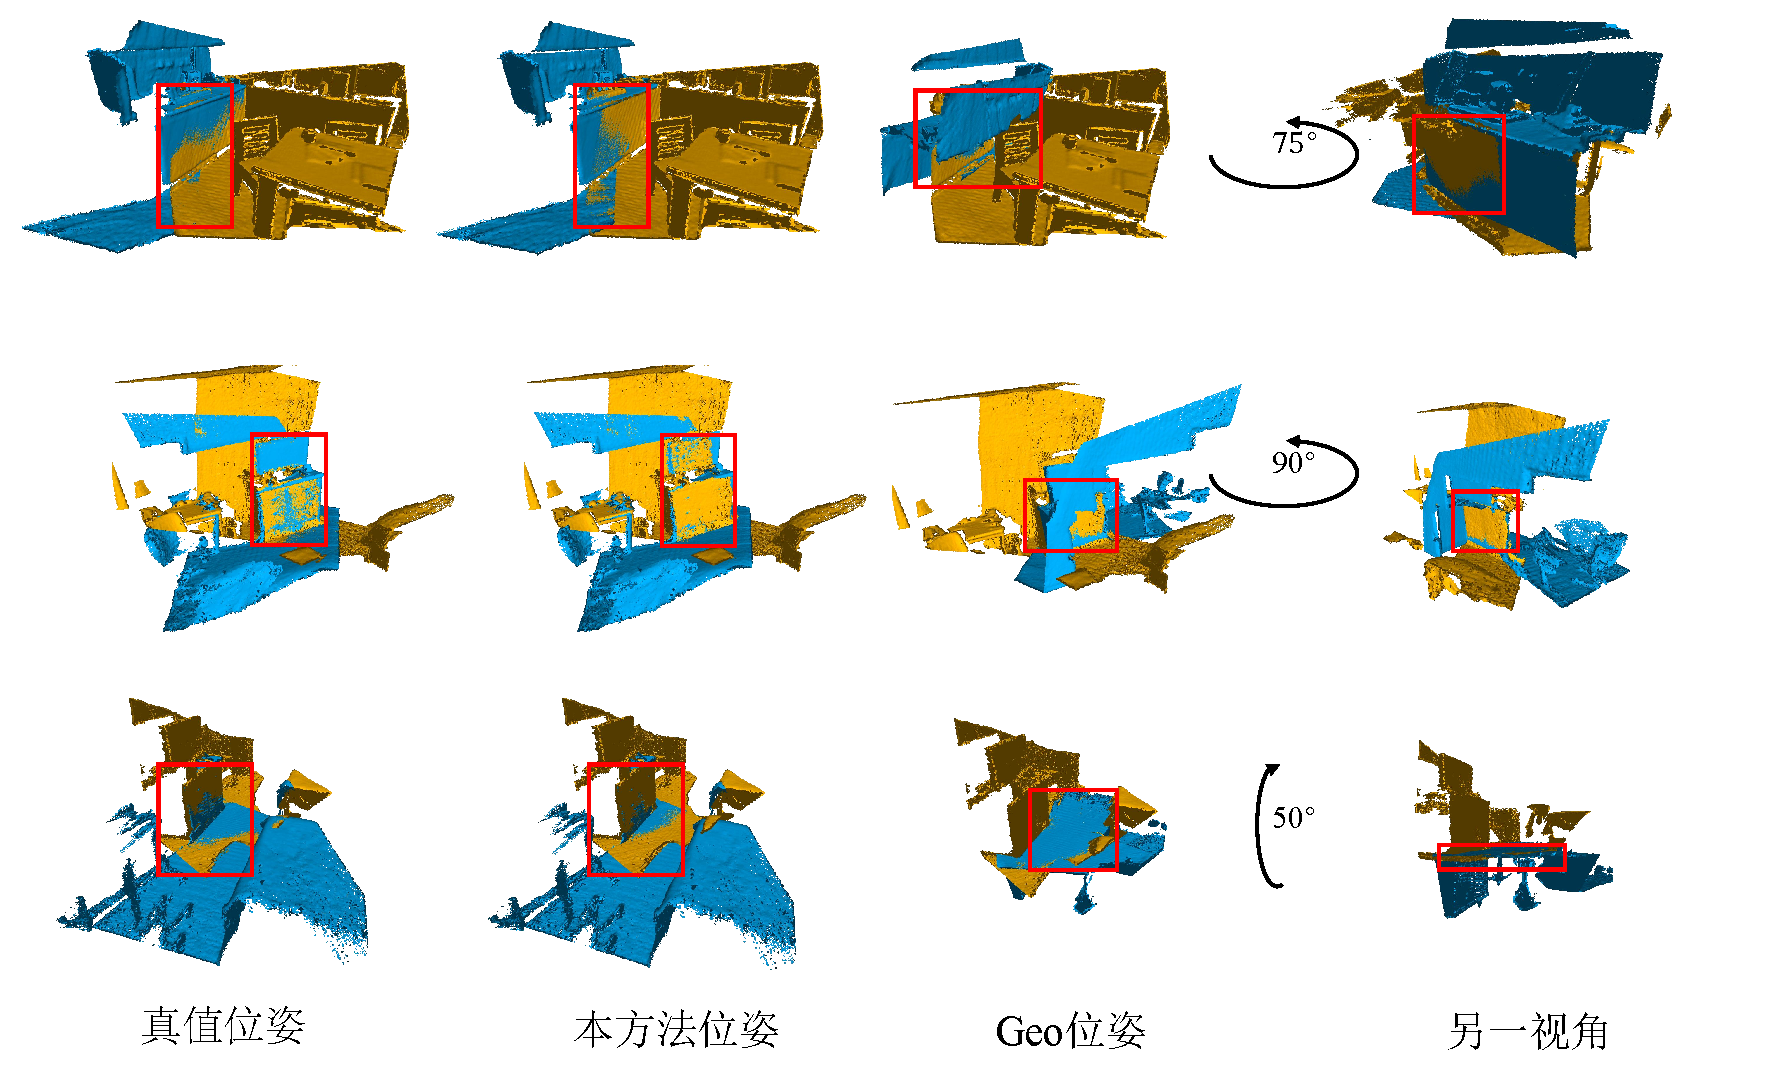
\includegraphics[width = \textwidth]{my/figure/3-6.pdf}
        \bicaption[\xiaosi 弱几何区域情况下与Geo的比较]{\wuhao 弱几何区域情况下与Geo的比较}{\wuhao The comparison of registration on low-geometry region against Geo}
        \label{fig:low_geometry}
    \end{figure}
    \vspace{-0.35cm}
    % 3DMatch和3DLoMatch的更多配准结果如图\ref{qualitative_registration_results}所示。输入源点云和目标点云、真值配准、Geo的配准以及我们的结果显示在(a)到(d)列中。
    % 前三行是3DMatch的配准,其余行是3DLoMatch的结果。我们可以看到,我们的方法对于这些具有挑战性的情况是稳健的,在不同的重叠比下存在大量外观相似的区域。这些定性结果进一步验证了我们方法的有效性。
    % \begin{figure}[h]
    %     \centering
    %     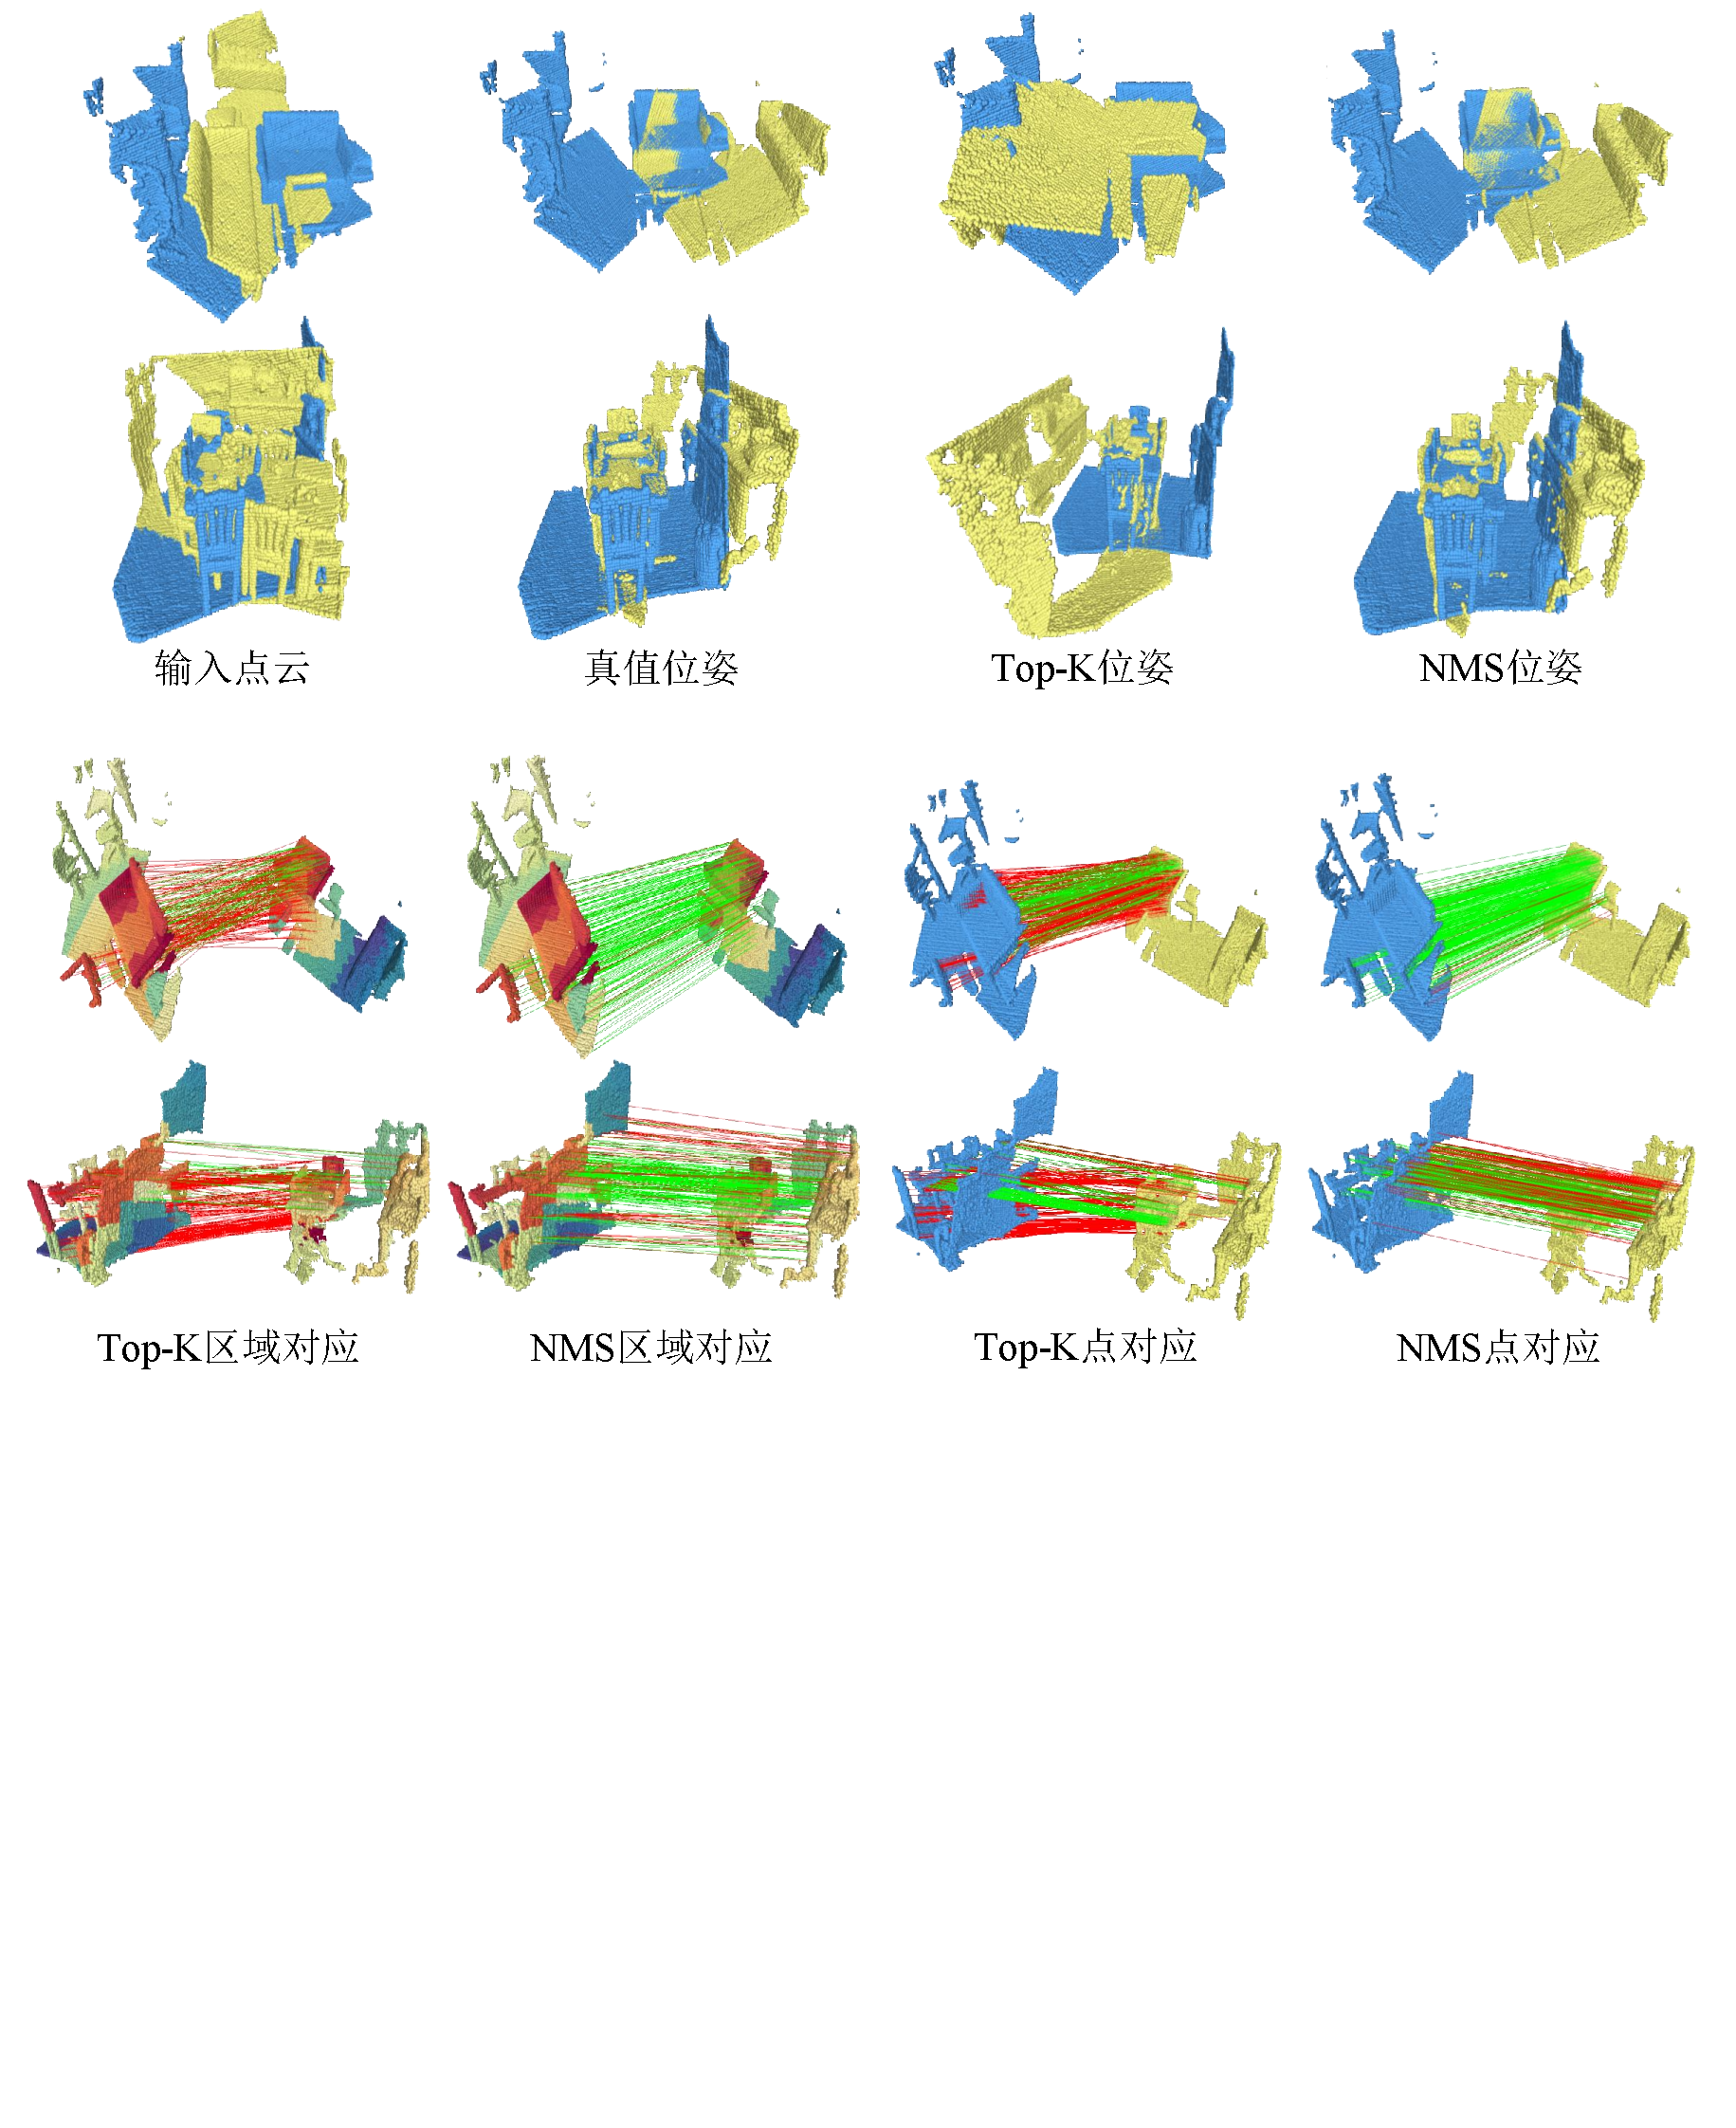
\includegraphics[width = \textwidth]{my/figure/3-7.pdf}
    %     \caption{\wuhao The 3DMatch和3DLoMatch上的配准结果可视化。}
    %     \wuhao Fig.3-7 visualization of registration results on 3DMatch and 3DLoMatch.
    %     \label{qualitative_registration_results}
    % \end{figure}

    \subsection{KITTI实验}
    \subsubsection{数据集与评价指标}
    KITTI是一个由11个室外场景序列组成的点云数据集。本文取序列0-5作为训练集,6-7作为验证集,8-10作为测试集。同时使用ICP算法在给定的GPS定位上进一步微调真值变换矩阵,在评估阶段使用间距至少为10m的点云对。\par
    本实验主要采用相对旋转误差(RRE)、相对平移误差(RTE)和配准召回率(RR)三个评估指标来评估模型的性能。
    % 相对旋转误差是预测配准结果与真实配准值之间的测地线距离。相对平移误差是预测配准结果和真实配准值之间的欧氏距离。
    与3DMatch和3DLoMatch的配准召回率不同,此处的配准召回率表示相对旋转误差和相对平移误差小于各自阈值的点云对的比例。\par
    \subsubsection{与最先进技术的比较}
    在KITTI数据集上,本文将基于LGR的方法与目前最先进的3DFeat-Net、FCGF、D3Feat、SpinNet、Predator、CoFiNet和Geo方法进行了比较。如表\ref{tab:kitti},虽然本方法在相对旋转误差方面表现一般,但本文基于LGR的模型在相对平移误差上实现了SOTA性能,比基于LGR的Geo和基于RANSAC的Predator低了0.6cm。实验表明,该模型在室外数据集上也具有一定的泛化能力。
    \begin{table}[h]
	\renewcommand{\arraystretch}{1}
    \centering
    \setlength{\tabcolsep}{7mm}{
    \bicaption[\xiaosi 最先进的方法和本方法在KITTI数据集上的性能比较。]{\wuhao 最先进的方法和本方法在KITTI数据集上的性能比较}{\wuhao Comparisons between the SOTA and this method on the KITTI}
    \label{tab:kitti}
    \wuhao

    \begin{tabular}{lccc}
    \toprule[1.5pt]
    Model          &RTE(cm)        &RRE($^\circ$) &RR(\%)
    \\ \hline
    3DFeat-Net
    & 25.9         & \ul{0.25}     & 96.0 
    \\
    FCGF
    & 9.5          & 0.30          & 96.6
    \\
    D3Feat
    & 7.2          & 0.30          & \textbf{99.8}
    \\
    SpinNet
    & 9.9          & 0.47          & \ul{99.1}
    \\
    Predator
    & \ul{6.8}     & 0.27          & \textbf{99.8}
    \\
    CoFiNet
    & 8.2          & 0.41          & \textbf{99.8}
    \\
    Geo(Ransac-50k)
    & 7.4          & 0.27          & \textbf{99.8}
    \\
    Geo(LGR)
    & \ul{6.8}     & \textbf{0.24} & \textbf{99.8}
    \\
    %Ours (Ransac-50k) & 9.6          & 0.33          & \textbf{99.8} \\
    Ours(LGR)
    & \textbf{6.2} & 0.30          & \textbf{99.8}
    \\
    \bottomrule[1.5pt]
    \end{tabular}
    }
\end{table}

    % 更多的可视化结果显示在图\ref{MGReg_ki}中。很明显,我们提出的方法允许对室外点云进行准确的配准。
    % \begin{figure}[h]
    %     \centering
    %     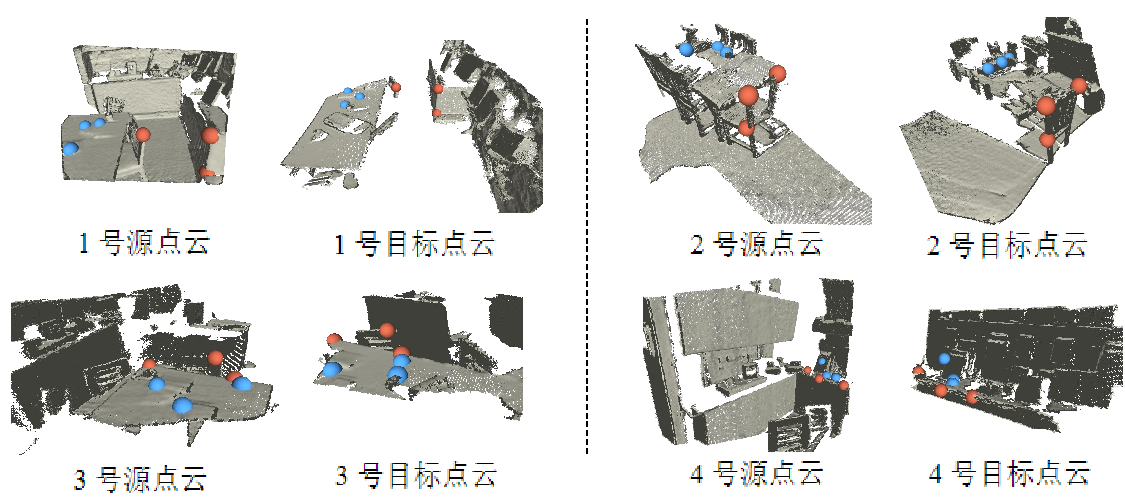
\includegraphics[width = \textwidth]{my/figure/3-8.pdf}
    %     \caption{\wuhao KITTI数据集配准结果的可视化.}
    %     \wuhao The visualization of registration  on KITTI odometry.
    %     \label{MGReg_ki}
    % \end{figure}

    \subsection{消融实验}
    本节设计了消融实验来分析网络中一些超参数和模块的有效性。消融实验使用的数据集为3DMatch和3DLoMatch,且使用局部到全局的配准(LGR)方法来计算变换矩阵。为了评估超点对应的质量,本节引入一个超点匹配的评价指标超点内点率(PIR),用来表示预测的超点对应之间的实际重叠率。\par

    \subsubsection{锚点定位模块的效果}
    如表\ref{tab:ablation_anchor_way},锚点定位模块可以有效增强几何嵌入的作用,进一步提高点云配准结果。在3DMatch数据集上,与Top-K选择显著锚点的方法相比,NMS的锚点定位模块可将超点内点率、特征匹配召回率、内点率和配准召回率分别提高0.7\%、0.6\%、0.1\%和0.2\%。在3DLoMatch上的提升更加明显,其中配准召回率能够提升1.8\%。
    \begin{table}[htp]
	\renewcommand{\arraystretch}{1}
    \centering
    \bicaption[\xiaosi 锚点定位模块消融实验]{\wuhao 锚点定位模块消融实验}{\wuhao Ablation experiments of the anchor location}\label{tab:ablation_anchor_way}
    \wuhao
    \begin{tabular}{ccccccccc}
    \toprule[1.5pt]
    \multirow{2}{*}{Model} & \multicolumn{4}{c}{3DMatch}  & \multicolumn{4}{c}{3DLoMatch} \\
    &{PIR} &{FMR} &{IR} &{RR}
    &{PIR} &{FMR} &{IR} &{RR}    \\ \hline
    {Top-K} & 85.8 & 97.7 & 70.8 & 91.5 & 54.3 & 86.3 & 43.5 & 73.3 \\
    {NMS}     & 86.5 & 98.3 & 70.9 & 91.7 & 55.7 & 86.5 & 44.1 & 75.1 \\ \bottomrule[1.5pt]
    \end{tabular}
\end{table}
    在使用Top-K方法选择锚点对应关系时,可能会有多个锚点相互靠近,导致这些锚点无法一定的几何结构,更严重的是可能多个锚点在空间中的聚集性会使得多个锚点的退化为一个锚点,从而削弱了选择性几何嵌入模块的几何嵌入效果。
    本节还在图\ref{fig:anchor_way}中比较了使用不同锚点选择方式的配准结果和对应关系可视化。可以观察到使用锚点定位模块能够产生更加稀疏的区域对应和点对应,同时这些对应关系的正确性也能够有所保证,这有助于更准确的配准结果。\par

    \vspace{-0.1cm}
    \begin{figure}[H]
        \centering
        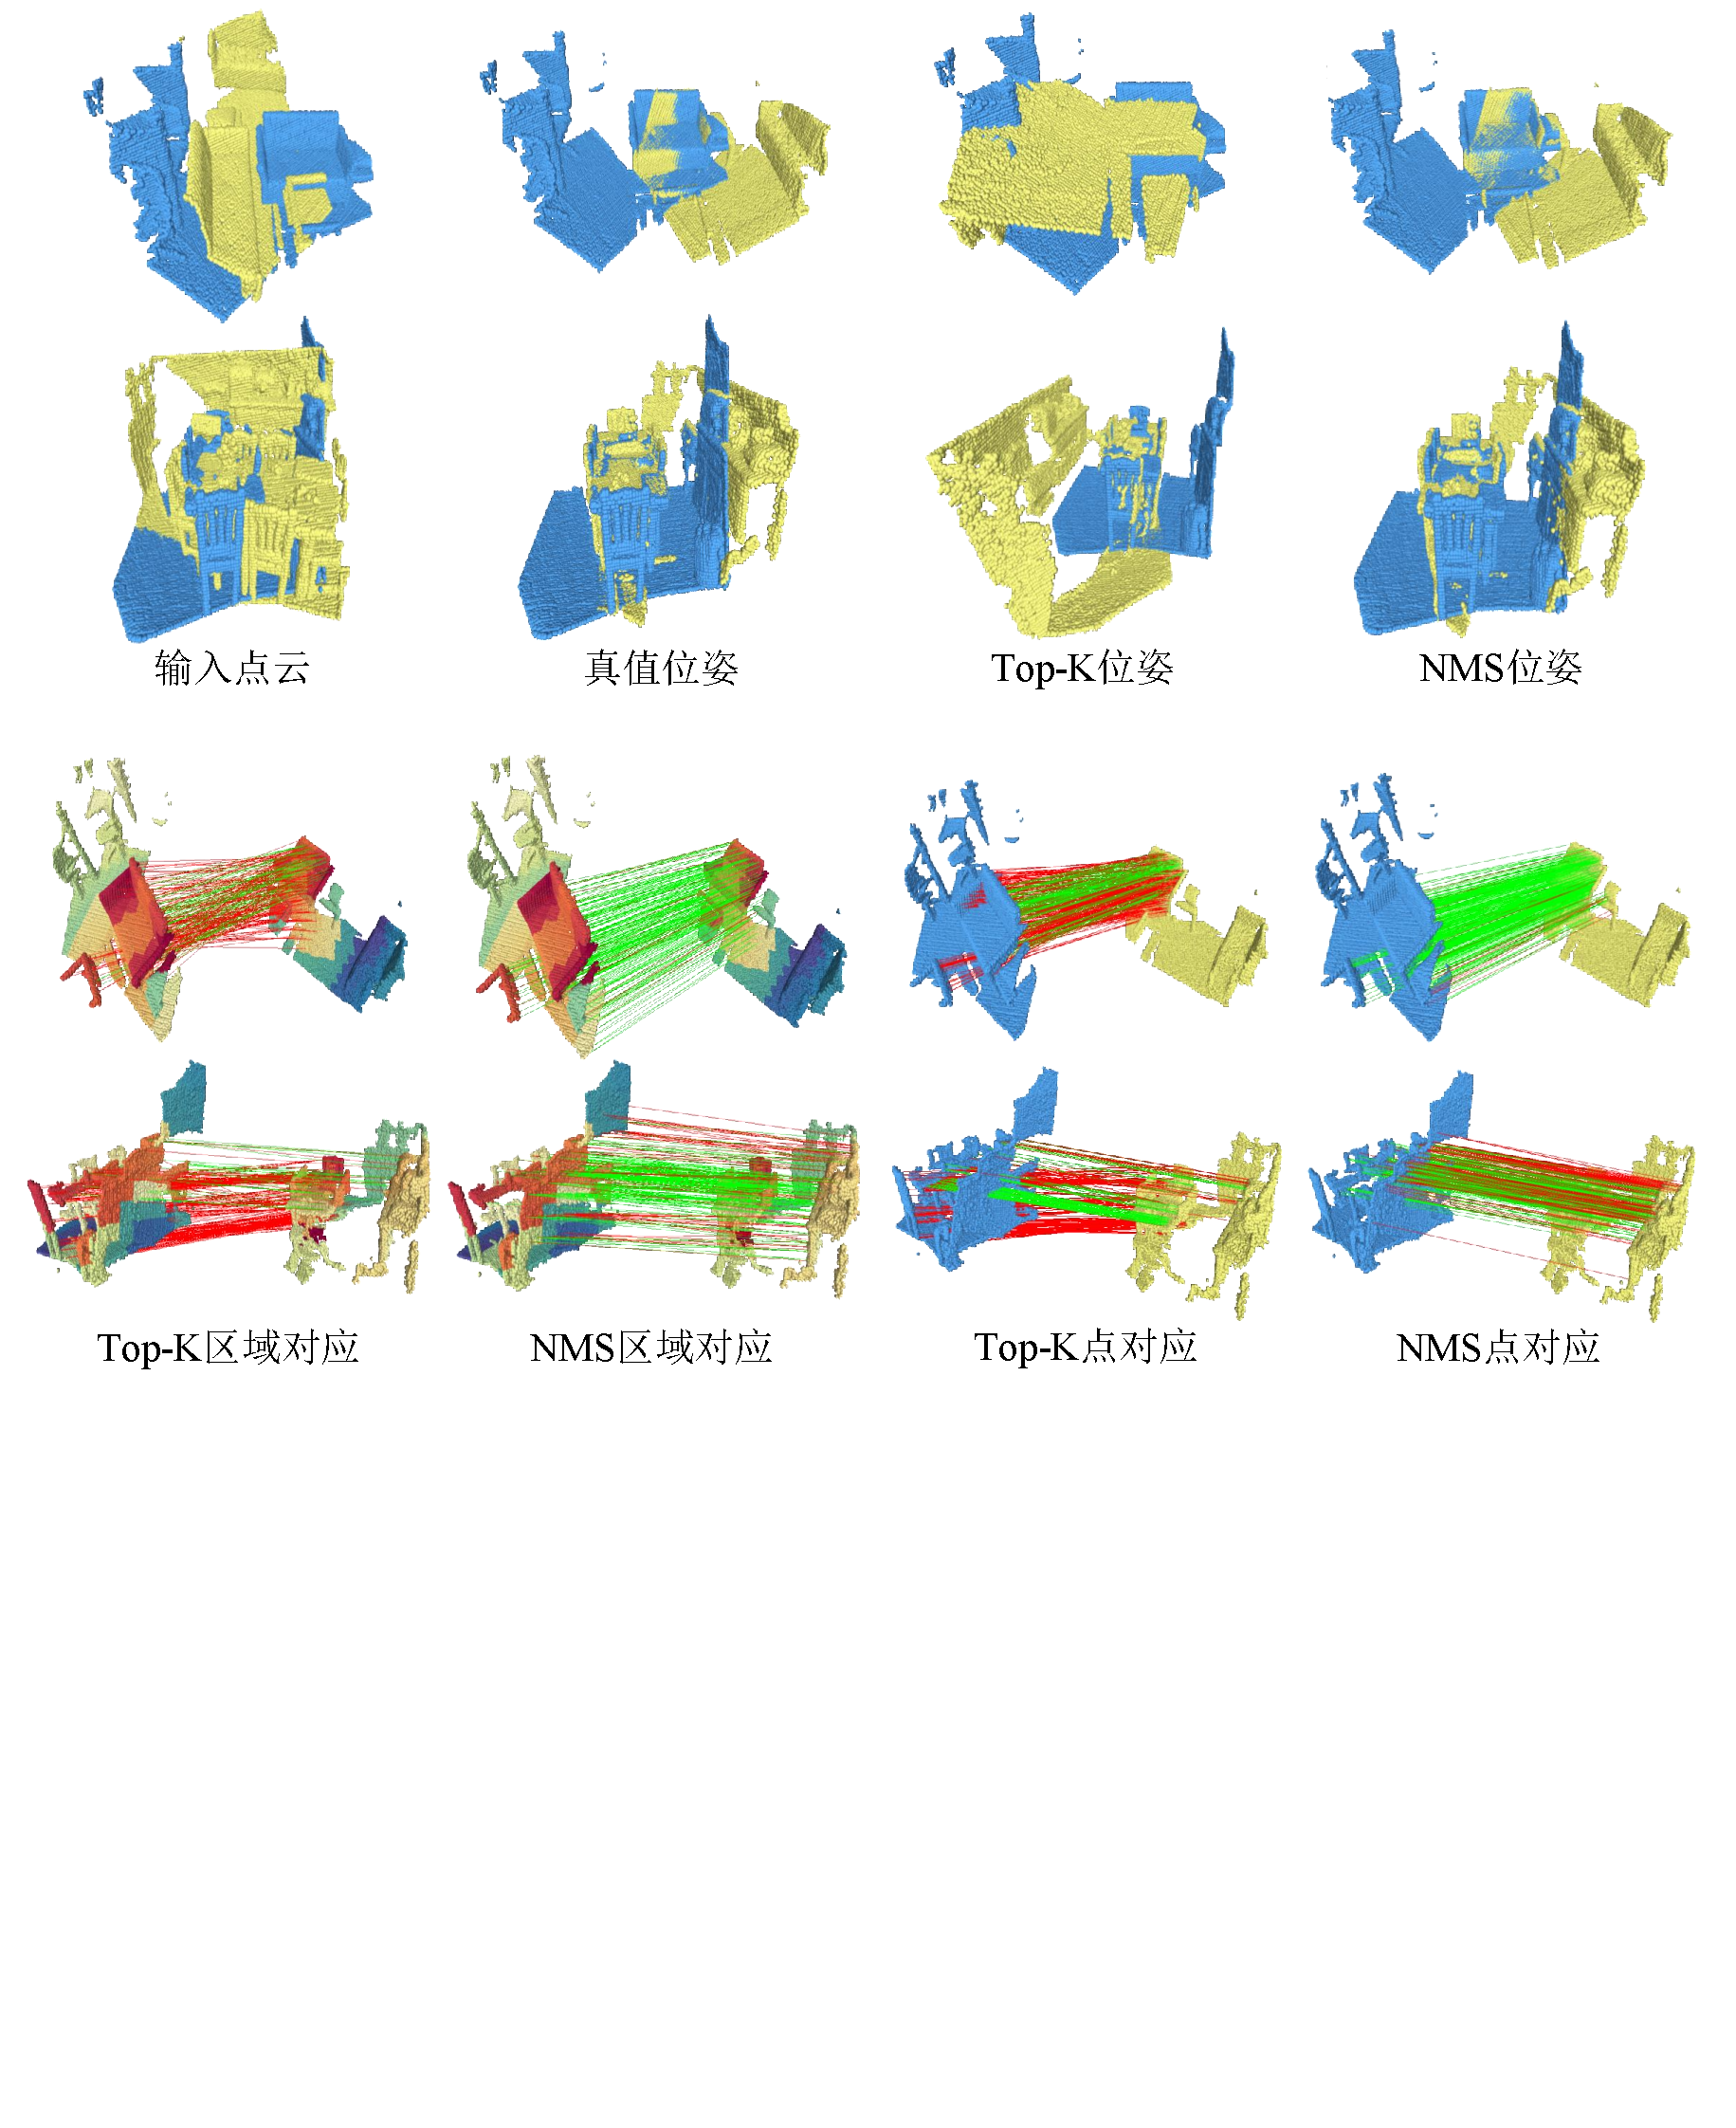
\includegraphics[width = \textwidth]{my/figure/3-7.pdf}
        \bicaption[\xiaosi NMS与Top-K锚点选择方法的配准结果的比较]{\wuhao NMS与Top-K锚点选择方法的配准结果的比较}{\wuhao Comparison of registration results using NMS and Top-K}
        \label{fig:anchor_way}
    \end{figure}
    \vspace{-0.35cm}

    \subsubsection{选择几何嵌入模块的效果}
    为了研究所提出的选择性几何嵌入模块的有效性,本节将其与仅使用自注意机制编码超点距离特征的基本模型进行比较。表\ref{tab:ablation_embedding}中的ED和EA分别表示距离嵌入和角度嵌入。通过在交叉注意上增加距离嵌入(+ED),3DMatch和3DLoMatch上的配准召回率分别提高了1\%和2.1\%。在此基础上进一步整合角度信息(+EA \& ED),3DMatch和3DLoMacth上的内点率分别提高了0.8\%和1.7\%。PIR也分别提高了1.9\%和1.5\%。更重要的是在3DLoMatch上的配准召回率也有0.9\%的提高。这意味着添加角度信息允许更准确的区域和点对应。因此,配准召回实现了最佳性能。该实验验证了选择性几何嵌入模块能够在真实的室内场景中提供有效的区分信息,基于锚点对应的点云间信息交互是有效的。\par
    \begin{table}[htp]
	\renewcommand{\arraystretch}{1}
    \centering
    \bicaption[\xiaosi 距离和角度嵌入对模型的影响]{\wuhao 距离和角度嵌入对模型的影响}{\wuhao The effect of distance and angle embedding on the model}\label{tab:ablation_embedding}
    \wuhao
    \begin{tabular}{lcccccccc}
    \toprule[1.5pt]
    \multicolumn{1}{c}{\multirow{2}{*}{Model}}
    & \multicolumn{4}{c}{3DMatch}
    & \multicolumn{4}{c}{3DLoMatch} \\
    \multicolumn{1}{c}{}
    & PIR   & FMR   & IR    & RR   & PIR   & FMR   & IR    & RR    \\ \hline
    baseline
    & 84.9  & 98.0  & 69.1  & 90.7 & 50.6  & 85.8  & 40.3  & 72.1  \\ 
    +ED
    & 84.6  & 98.3  & 70.1  & 91.7 & 54.2  & 86.8  & 42.4  & 74.2  \\ 
    +EA \& ED
    & 86.5  & 98.3  & 70.9  & 91.7 & 55.7  & 86.5  & 44.1  & 75.1  \\
    \bottomrule[1.5pt]
    \end{tabular}
\end{table}

    \subsubsection{基于迭代优化的显著锚更新效果}
    如表\ref{tab:ablation_iteration},在3DLoMatch上,迭代次数为2时的配准召回率比迭代次数为1的配准召回率高1.5\%,迭代次数为3的性能比迭代次数为2的性能低1\%。本文分析,随着迭代次数的增加,锚点的采样在一些不同的区域。

    当重叠率较低时,锚点不可避免地会集中。锚点集中后,嵌入的特征失去了差异,导致性能下降。这一点可以从\ref{tab:ablation_iteration}中的3DMatch实验中得到验证。当重叠率较高时,锚点分布相对均匀,不会造成性能下降。

    \begin{table}[h]
	\renewcommand{\arraystretch}{1}
    \centering
    \bicaption[\xiaosi 迭代次数对模型的影响]{\wuhao 迭代次数对模型的影响}{\wuhao The effect of the number of iterations on the model}\label{tab:ablation_iteration}
    \wuhao
    \begin{tabular}{ccccccccc}
    \toprule[1.5pt]
    \multicolumn{1}{l}{\multirow{2}{*}{Iteration}} 
    & \multicolumn{4}{c}{3DMatch}
    & \multicolumn{4}{c}{3DLoMatch} \\
    \multicolumn{1}{l}{}
    &{PIR} &{FMR} &{IR} &{RR}   
    &{PIR} &{FMR} &{IR} &{RR}    \\ \hline
    1
    & 75.1  & 98.8  & 64.4  & 91.3 & 44.6  & 87.8  & 37.1  & 73.6  \\
    2
    & 86.5  & 98.3  & 70.9  & 91.7 & 55.7  & 86.5  & 44.1  & 75.1  \\
    3
    & 87.2  & 97.9  & 71.8  & 91.4 & 57.3  & 86.6  & 45.3  & 74.1  \\
    \bottomrule[1.5pt]
    \end{tabular}
\end{table}

    本文还在图\ref{fig:ablation_iteration}中可视化源点云和目标点云中锚点的位置。蓝色球体是执行IOSAU之前的锚点位置,橙色球体是执行IOSAU之后的锚点位置。可以看到最初的锚点位于那些弱几何区域,如图\ref{fig:ablation_iteration}中第一行的两个例子中的桌面。但是,在进行基于迭代的优化更新后,可以看到更新后的锚点位于显著区域,如角落或尖锐的边界。这样,超点相对于显著锚点的几何嵌入具有明显的区别性,可以提高特征的区别度。

    \vspace{-0.1cm}
    \begin{figure}[h]
        \centering
        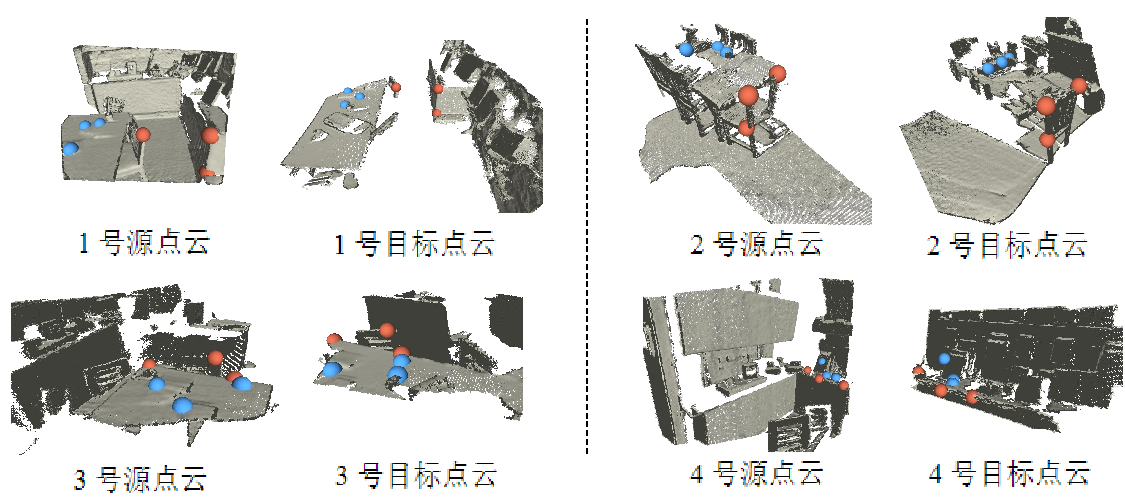
\includegraphics[width = \textwidth]{my/figure/3-8.pdf}

        \captionsetup{margin = {1.6cm, 1.6cm}}
        \bicaption[\xiaosi 基于迭代优化显著锚点更新前后源点云和目标点云中锚点位置的可视化]{\wuhao 基于迭代优化显著锚点更新前后源点云和目标点云中锚点位置的可视化
        % 。(a)1号源点云;(b) 1号目标点云;(c) 2号源点云;(d) 2号目标点云;(e) 3号源点云;(f) 3号目标点云;(g) 4号源点云;(h) 4号目标点云
        }{\wuhao Visualization of the location of anchor points in the source and target point clouds before and after iteration-based optimisation salient anchor updating
        % .(a) No. 1 source point cloud; (b) No. 1 target point cloud; (c) No. 2 source point cloud; (d) No. 2 target point cloud; (e) No. 3 source point cloud; (f) No. 3 target point cloud; (g) No. 4 source point cloud; (h) No. 4 target point cloud
        }
        \label{fig:ablation_iteration}
        % The blue spheres are the initial anchors before IOSAU. The red ones are the salient anchors after IOSAU.
    \end{figure}
    \vspace{-0.35cm}

    \section{本章小结}
    本文提出了一种基于显著锚点几何信息嵌入的鲁棒点云配准方法。利用分布稀疏且保持一定几何结构的锚点,选择性嵌入锚点与超点间的距离和角度的几何特征,增强特征间的差异性,实现精确的超点匹配。为了将最明显的信息融合到特征中,本章还提出了一种基于迭代优化的显著锚点更新,以实现最有效和最准确的几何嵌入。
    该方法以锚点对应为媒介,在源点云和目标点云之间交换几何信息。即使是在非重叠部分的外观相似区域,以及重叠部分的几何形状较弱的区域也能通过嵌入显著锚点对应相关的上下文信息实现准确可靠的区域对应。在室内和室外基准上进行的大量定量和定性实验验证了本章方法的有效性。

% 第4章
\chapter{基于多模态特征融合的锚点定位点云配准}
\thispagestyle{others}
\pagestyle{others}
\xiaosi

    \section{本章引言}
    点云中广泛存在可重复且模糊的结构,例如地板、墙壁和天花板都是平面。这些可重复且不明确的结构信息将在很大程度上影响特征的独特性、差异性。因此,只考虑点云结构信息的神经网络预测出来的对应关系中包含大量的离群值。如何提高点云特征的区分度是当前点云配准方法的主要研究方向。

    在早期研究阶段,大多数方法要么对几何结构进行充分的发掘和利用,要么参考图像配准方法开发新的配准框架,往往忽略了来自图片的纹理信息。二维图像虽然缺乏距离和角度等立体空间信息,但是其提供的颜色纹理等内容是人类理解世界的重要组成部分。近年来在3D目标检测和位置识别等领域越来越多的研究人员考虑将图像信息与点云信息融合起来。多模态信息融合的基本理论是利用模态信息间的互补性实现信息的相互补充提高特征的鲁棒性。就点云和图像而言,点云数据缺乏颜色信息和纹理信息但是对物体与环境的拓扑结构有着良好的表示,图像数据便能够作为有效的补充数据对点云数据进行补充。

    % 文献\cite{FPointNet}和文献\cite{F-ConvNet}将点云和图像进行拼接融合,首先通过标准的2D CNN特征提取器提取图像特征并于点云拼接,然后使用类似PointNet的模块进行回归分割和筛选每个点。
    % 相比之下,更多的研究同时完成了这一任务。
    文献\cite{9156790, 7780605}通过用逐点的2D分割特征增强3D坐标来进行数据级融合;文献\cite{8100174, 8594049}通过简单的拼接或特定模块实现来自单个网络的2D和3D表示的特征级融合。与仅使用激光雷达的方法不同,这种方法在单点云模式下不断更新更复杂的设计模型和更合适的训练方案,多模态替代方案努力利用更多样化的信息,并显示出巨大的潜力。

    尽管使用多模态的方法来进行特征提取受到越来越多的研究者的青睐,但是随之带来的挑战是不同模态之间存在着模态差异,如何更好的融合来自多种模态的信息是重点的研究方向。据调查发现,在3D目标检测的同行研究中,虽然研究人员期望这两种传感器的组合能够提供更好的性能,但事实证明,大多数最先进的3D物体探测器仅使用激光雷达作为输入。这表明如何有效地融合来自这两个传感器的数据仍然具有挑战性。
    虽然激光雷达点云和RGB图像具有互补的信息,但是由于两种模态的数据存在较大的域间隙,实现信息的互补并不容易。
    % 同时,当前算法往往使用卷积神经网络提取图像特征之后,将像素特征与原始点云进行简单拼接并输入点云骨干网络以完成特征融合,这进一步限制了融合效果。

    这种差距的出现主要由三方面造成:(1)点云和图像特征提取的网络之间存在较大差异,用于提取点云特征的网络往往针对点云数据的无序性,不规则性和稀疏性设计,而图像特征提取网络主要利用卷积对图像的结构和纹理信息进行提取,因此两种模态数据的特征之间存在着较大鸿沟,导致了融合过程中信息的丢失。(2)当前算法往往使用卷积神经网络提取图像特征之后,将像素特征与原始点云进行简单拼接并输入点云骨干网络以完成特征融合,这进一步限制了融合效果。这使得不同模态特征的相关性被忽略了,关键信息没有有效的突出。(3)数据增强技术被广泛应用于各种任务当中,但是对于多模态融合来说这种简单的机制可能不会有效的提高算法性能,这主要是由于对多模态而言对齐两种模态的数据是非常重要的,通过旋转平移等数据增强操作往往会造成模态间数据的错位。

    综上所述,本章为了提高点特征的区分度设计了一个点云图像融合的点云配准框架。提出了一个对齐模块将数据增强后的两种模态数据进行像素与超点间的对齐。提出一种新的多模态融合方法,先后在模态无关和模态相关两个子空间对点云特征和图像特征进行融合,减少模态间的域间隙和信息丢失。

    % 现有的最先进的点描述符仅依赖于结构信息,忽略了纹理信息。然而,纹理信息对于我们人类区分场景部分是至关重要的。本文提出了一种同时考虑结构和纹理信息的多模态融合方法来生成点云配准描述子。
    % 具体而言,设计了一种新的注意力融合模块,用于提取加权纹理信息,用于描述符提取。本文进一步解释了注册任务中的深度学习。在3DMatch、3DLoMatch和KITTI上的综合实验表明,多模态融合描述子达到了最先进的精度,提高了描述子的显著性。


    % 三维点描述符的特殊性决定了这些基于描述符的配准方法的性能。
    % 目前大多数3D描述符利用结构信息来描述点[1,5,12,20]。
    % 然而,点云中广泛存在可重复且模糊的结构,例如地板、墙壁和天花板都是平面(如图1所示)。这些可重复且不明确的结构信息将在很大程度上影响描述符的独特性。因此,通过比较仅结构的点描述符估计的对应关系包含显著的异常值。现有已发表的文献[1,5,12]已经证明了这种现象,当inlier阈值增加到0.2时,特征匹配召回率下降了很多。
    % 为了提高点描述子的独特性,提出了一种新的多模态融合方法,通过融合点云的结构信息和对应图像的纹理信息来学习三维点描述子。我们的动机在于,当我们观看一个场景时,我们通常会同时考虑纹理和结构,并区分两个部分——例如,红色的墙壁(Ip)和黄色的地板(Iq)(如图1所示)。
    % 具体来说,我们的多模态融合方法是基于FCGF[5]的编码器和解耦器架构。受变压器[22]的启发,在编码器模块之后,开发了一种新的交叉注意模块来提取每个点的加权纹理信息。然后,我们将纹理和结构信息连接起来,并将它们馈送到解耦器模块中进行最终的描述符学习。
    % 本文的主要贡献可以概括为:•提出了一种新的多模态融合方法来学习具有纹理和结构信息的三维点描述符。我们的方法将提高描述符的独特性。
    % •综合实验表明,所提出的多模态融合描述子在室内和室外数据集上都达到了最先进的性能。//IMFNet

    % 在本文中,我们提出了两种新技术:反演几何相关的增强(例如旋转),以实现激光雷达点和图像像素之间的精确几何对齐,以及LearnableAlign,利用交叉注意动态捕获融合过程中图像和激光雷达特征之间的相关性。基于InverseAug和LearnableAlign,我们开发了一系列通用的多模态3D检测模型,命名为DeepFusion,它比以前的方法更准确。

    % 文献中用于融合激光雷达和相机的现有方法大致遵循两种方法(图1):它们要么在早期阶段融合特征,例如用相应的相机特征装饰激光雷达点云中的点[34,36],要么使用中级融合,在特征提取后将特征组合在一起[13,17]。

    % 在这两种方法中最大的挑战之一是找出激光雷达和相机功能之间的对应关系。为了解决这个问题,我们提出了两种方法:InverseAug和LearnableAlign来实现有效的中层融合。InverseAug反演几何相关的数据增强,然后使用原始相机和激光雷达参数将两种模式关联起来。LearnableAlign利用交叉注意动态学习激光雷达特征与其对应的相机特征之间的相关性。这两种技术简单、通用、高效。基于PointPillars[16]和CenterPoint[44]等流行的3D点云检测框架,InverseAug和LearnableAlign可以帮助相机图像以边际计算成本(即只有一个交叉注意层)有效地与激光雷达点云对齐。当融合对齐的多模态特征时,摄像机信号具有更高的分辨率,显著提高了模型的识别和定位能力。这些优点尤其有利于远距离目标检测。
    % 我们开发了一系列名为deepfusion的多模态3D检测模型,其优势在于:(1)可以端到端训练,(2)是与许多现有的基于体素的3D检测方法兼容的通用构建块。DeepFusion作为一个插件,可以很容易地应用于大多数基于体素的3D检测方法,如PointPillars[16]和CenterPoint[44]。
    % 我们的大量实验表明(1)有效的深度特征对齐是多模态三维物体检测的关键,(2)通过我们提出的InverseAug和LearnableAlign提高对齐质量,DeepFusion显著提高了检测精度,(3)与单模态基线相比,DeepFusion对输入破坏和分布不均匀的数据更加稳健。
    % 在Waymo开放数据集上,DeepFusion改进了几个流行的3D检测模型,如PointPillars [16], CenterPoints[44]和3D- man[43],分别提高了6.7,8.9和6.2 LEVEL 2 APH。我们在Waymo开放数据集上取得了最先进的结果,DeepFusion在验证集上比之前最好的多模态方法pointaug[36]提高了7.4 Pedestrian LEVEL 2 APH。这一结果表明,我们的方法能够有效地结合激光雷达和相机模式,其中最大的改进来自于对远距离目标的识别和定位。
    % 我们的贡献可以概括为三个方面:•据我们所知,我们是第一个系统地研究深度特征对齐对3D多模态检测器的影响的人;•我们提出InverseAug和LearnableAlign来实现深度特征级对齐,从而实现准确和鲁棒的3D物体检测器;•我们提出的模型deepfusion在Waymo开放数据集上实现了最先进的性能。//deepfusion

    % 为了解决这一问题,我们提出了一个新的框架,即用于多模态3D目标检测的对比增强变压器(CAT-Det)。具体来说,CATDet采用了由Pointformer (PT)分支、Imageformer (IT)分支和Cross-Modal Transformer (CMT)模块组成的双流结构。PT、IT和CMT联合编码了表示对象的模内和模间长程上下文,从而充分探索了用于检测的多模态信息。此外,我们提出了一种有效的单向多模态数据增强(OMDA)方法,通过点级和对象级的层次对比学习,仅通过增强点云即可显著提高精度,而无需复杂地生成两种模态的配对样本。在KITTI基准上进行的大量实验表明,CAT-Det达到了新的最先进水平,突出了其有效性。

    % 为了解决上述问题,本文提出了一种新的多模态三维目标检测框架,即对比增强变压器检测器(CA T-Det)。它采用双流结构,由Pointformer (PT)分支、Imageformer (It)分支和Cross-Modal Transformer (CMT)模块组成。与pointnet++和cnn不同的是,PT和IT分支都拥有较大的接受域,分别能够在点云和图像中捕获丰富的全局上下文信息,加强硬样本的特征。随后,CMT模块进行跨模态特征交互和多模态特征组合,通过整体学习的细粒度权重充分强调两种模态提取的基本线索。PT、IT和CMT的集成充分编码了模态内和模态间的长期依赖关系,从而提高了检测性能。此外,我们提出了一种单向多模态数据增强(OMDA)方法,该方法通过分层对比学习,仅在点云模态上执行即可实现有效的增强。
    % 综上所述,本文的主要贡献是:(1)我们提出了一种新的CA T-Det框架,用于多模态三维物体检测,它包含一个点前分支、一个图像前分支和一个跨模态转换器模块。据我们所知,这是将变压器结构应用于给定任务的第一次尝试。(2)我们提出了一种单向数据增强的多模态三维目标检测方法,通过分层对比学习,仅通过增强点云就能显著提高精度,从而避免了两种模态成对样本的复杂生成。(3)我们在KITTI测试集上实现了所有三个类别的最新最先进的mAP,并与已发表的同类进行了比较,并证明了其在检测硬物体方面的优势。

    \section{基于多模态特征融合的锚点定位点云配准方法}
    为了更有效的提高源点云和目标点云相似非重叠区域特征间的特征差异性,本章提出了一个基于多模态特征融合点云配准新框架,整个方法遵循图\ref{fig:4-1}所示的基于多模态融合的点云配准新框架结构。

    \vspace{-0.1cm}
    \begin{figure}[h]
        \centering
        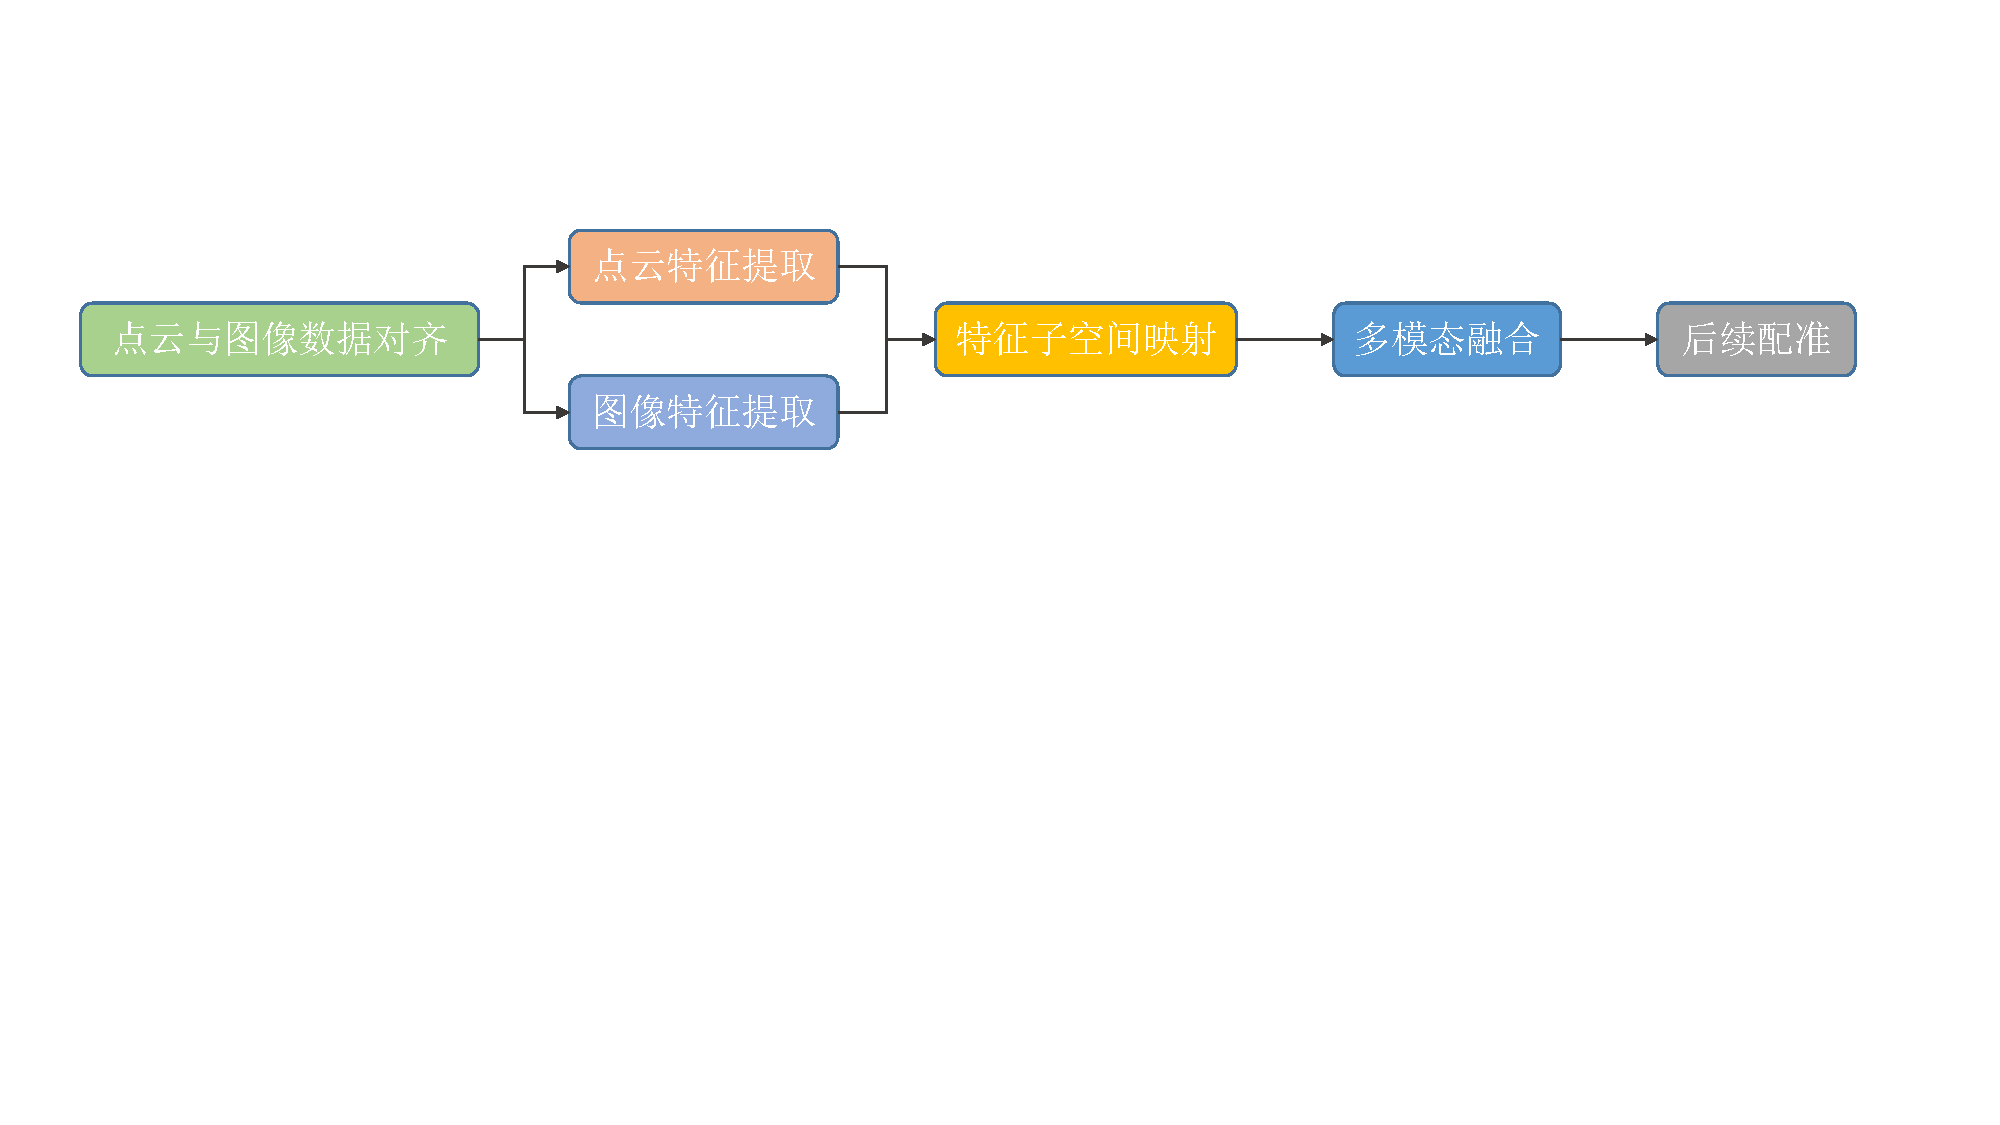
\includegraphics[width = \textwidth]{my/figure/4-1.pdf}
        % \captionsetup{margin = {1.6cm,1.6cm}}
        \bicaption[\xiaosi 第四章方法示意图]{\wuhao 本方法示意图}{\wuhao Schematic diagram of the method}
        \label{fig:4-1}
    \end{figure}
    \vspace{-0.35cm}

    图\ref{fig:4-2}展示了整个方法的示意图。该方法主要包括三个步骤:(1)在特征提取之前进行数据对齐,将点云和对应图像间的空间位置对齐即将点云中点的坐标投影至图像中,寻找点与像素之间的对应关系;(2)从点云中提取出超点的局部几何特征,并从各自对应的图像中提取二维纹理特征;(3)最后使用基于注意力机制的融合模块,将点云中的超点的特征与对应像素的纹理特征相融合,得到融合特征。
    随后操作与第三章中的方法一致,通过融合后的特征寻找具有显著特征且位于重叠区域的锚点,然后利用自注意力和交叉注意力机制对点云的几何结构特征进行编码,接着通过迭代优化更新显著超点与超点特征,最终将超点匹配扩充为点匹配并估计变换矩阵。

    基于多模态特征融合的锚点定位点云配准方法的重点在强调点云和图像间数据的对齐作为多模态融合的前置操作,经过对齐模块能够寻找到点云中的点与对应图像中像素的对应关系,相比于使用全局融合,这种融合方法是能够更加准确的有效的融合点的颜色纹理信息。许多以前的方法都没有在多模态融合之前进行额外的操作,这使得他们的融合效果受到限制;同时该方法在融合之前将模态数据投影到两个子空间中,通过减少域间隙融合两种不同模态的数据能够减少冗余信息对特征的干扰,使得多模态融合的效果更好。

    \vspace{-0.1cm}
    \begin{figure}[h]
        \centering
        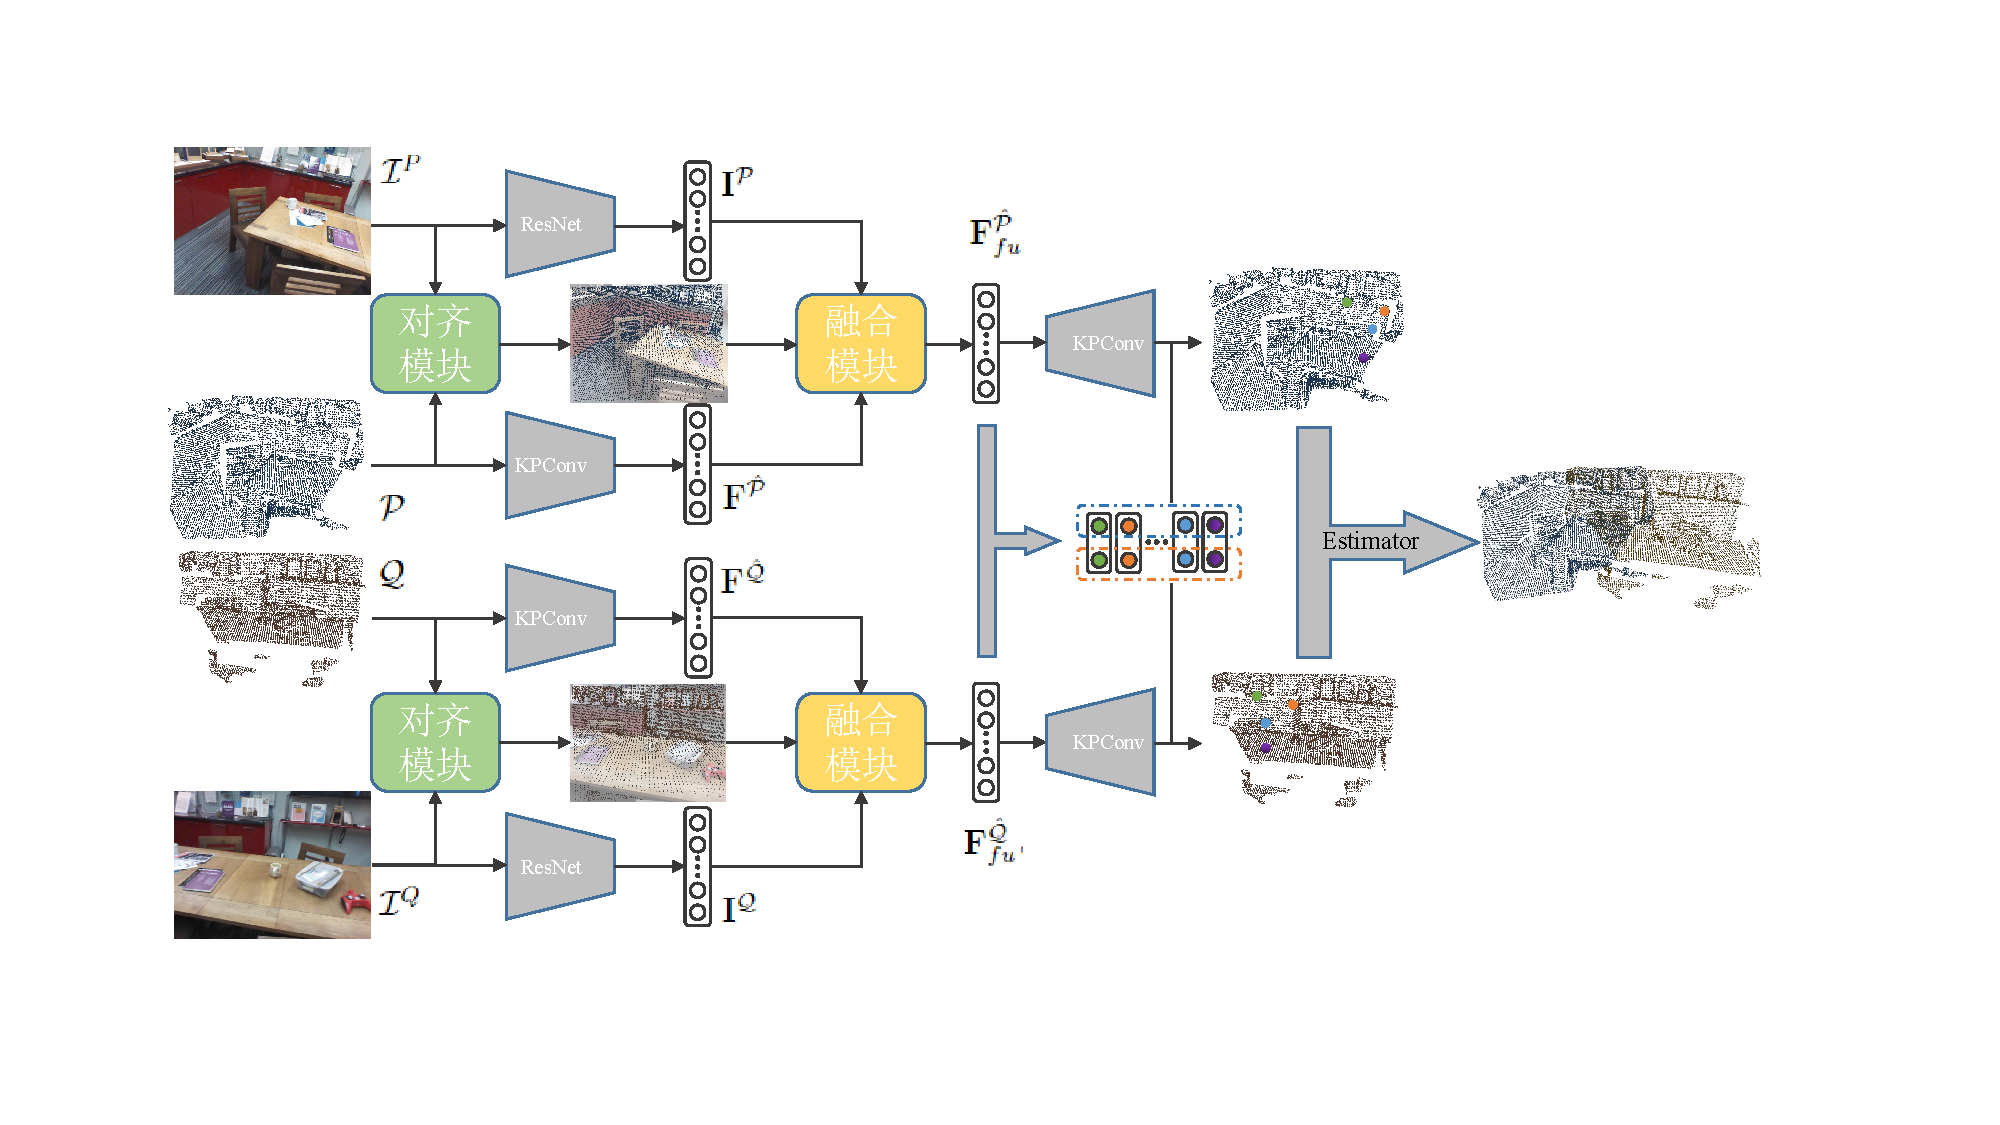
\includegraphics[width = \textwidth]{my/figure/4-2.pdf}
        % \captionsetup{margin = {1.6cm,1.6cm}}
        \bicaption[\xiaosi 第四章方法框架图]{\wuhao 本方法框架图}{\wuhao Overview of the proposed registration method}
        \label{fig:4-2}
    \end{figure}
    \vspace{-0.35cm}

    该方法的贡献如下:(1)对于点云和图像模态,使用对齐模块将点云和图像之间的数据对齐,具体而言将点云投影至二维平面并与图像对齐,寻找到超点与像素之间的一种一对多的对应关系;(2)在多模态融合之前,将投影两种模态的数据到正交的子空间,并先后融合两种模态数据学习跨模态的信息。

    \subsection{对齐模块}
    为了训练图像和点云数据,本文提出了一个融合模块,用于将图像的纹理颜色和点云的几何结构进行融合。因此,需要找到点云中的点和图像中的像素之间的对应关系。从三维空间到二维图像有一个成像过程,本模块通过将三维点云投影到二维图像,以便精确的寻找到点和像素之间的映射关系,促进后续两种模态特征的融合。对于源点云$\mathcal{P}$和源点云对应的图像$\mathcal{I}^\mathcal{P}$而言,它们之间的成像过程可以由公式(4-1)表示:
    \begin{equation}
        \mathcal{I}^\mathcal{P} = \mathbf{K}_{in} \mathbf{T}_{ex} \mathcal{P}
    \end{equation}
    式中,$\mathbf{K}_{in}$表示相机的内参矩阵;$\mathbf{T}_{ex}$表示相机的外参矩阵。对于未经过数据增强的点云和图像而言外参矩阵$\mathbf{T}_{ex}$为4阶单位矩阵,$\mathbf{K}_{in}$则与相机本身相关且不受到数据增强的影响。\par

    一种处理方式是不对点云数据进行数据增强处理,然而这种简单的处理方法会使模型在训练过程中陷入过拟合。本方法为了避免模型过拟合依旧采用随机旋转和增强噪音等策略。然而这时如果不采用额外的处理,依旧使用4阶单位矩阵作为外参矩阵$\mathbf{T}_{ex}$,那么点云的投影和图像之间将会存在偏差,这将导致点的颜色信息被错误的融合了,进一步到整体模型性能的下降。文献\cite{Deepfusion}指出数据增强对模型的促进作用将会随着随机旋转角度的增大而下降。这也进一步表明在特征融合之前对齐点云和图像两种模态的数据是至关重要的。

    为了解决数据增强带来的对齐偏差问题,本文提出了一个模态对齐模块。为了使重定位可行,对点云进行数据增强后,首先保存数据增强相关参数比如旋转角度。在对齐阶段,它将这些数据增强进行反转,得到输入点云中的三维空间点的原始坐标,然后在相机空间中找到其对应的二维坐标。由于本方法采用的是又粗到细的配准框架,即在提取点云特征过程中将点云下采样为超点。超点与原始点之间存在一对多的关系,而原始点与像素存在一对一的关系,因此最终本模块将得到超点与像素之间的一对多的对应关系。这种对应关系表示一个超点是图像中某块区域。最终,本节将得到超点与像素之间的对应关系矩阵$\mathbf{C}^{\hat{P}} \in \mathbb{R}^{N' \times L}$。同理本节会得到目标点云与其图像间的对应关系$\mathbf{C}^{\hat{Q}} \in \mathbb{R}^{M' \times L}$。

    % 当前许多将点云和图像数据融合的多模态方法往往通过图像特征提取器提取图像特征之后,利用图像特征修饰原始点云,再将修饰后的点云输入点云特征提取其中提取后续任务所需要的点云特征。然而这种方法忽略了图像特征提取器与点云特征提取器之间的域间隙,这种前融合方式并没有对图像和点云的特点进行分析导致融合后的特征并不能有效提高最终性能。
    % 综上,本章采用一种后融合的方式来深度融合点云和图像,分别通过点云和图像的特征提取器提取点云特征和图像特征;然后将两种模态的特征融合;最后将融合后的特征通过基于显著锚点几何嵌入的点云配准框架的其他组件得到最终的配准结果 。
    % 与之前的方法相比本章的融合方法能够有效缓解模态间的域间隙问题。然而,缺点也很明显,与输入级装饰相比,在深度特征层面上,将图像特征与点云特征对齐变得并不直接。例如,两种模态的异构数据增强导致的不准确对齐可能对融合阶段构成潜在挑战。

    \subsection{多模态特征提取}
    该方法的另一模块是多模态特征提取,而多模态特征的提取的核心是从点云和是图像当中提取出能够很好地代表点云局部结构和图像纹理信息的特征。本研究将源点云和目标点云输入到KPConv网络中,该网络能过够在提取特征的同时将点云下采样为超点。另一方面,本方法将对应的图像输入到用于提取像素特征的标准的ResUNet骨干网络中。选择ResUNet主要是因为可以加载该网络的最流行的预训练模型。这种由大数据集训练而来预训练模型,能够使网络起初就拥有良好的图像特征,同时使网络在训练过程中更加稳定。

    具体的网络结构遵循CofiNet使用KPConv稀疏卷积网络。输入源点云$\mathcal{P} \in \mathbb{R}^{N \times 3}$和目标点云$\mathcal{Q} \in \mathbb{R}^{M \times 3}$,输出$\mathbf{F}^{\hat{\mathcal{P}}} \in \mathbb{R}^{N' \times d}$和$\mathbf{F}^{\hat{\mathcal{Q}}} \in \mathbb{R}^{M' \times d}$。
    输入是源点云和目标点云对应的图像
    $\mathcal{I}^P \in \mathbb{R}^{W \times H \times 3}$ 和
    $\mathcal{I}^Q \in \mathbb{R}^{W \times H \times 3}$,
    输出是其特征
    $\mathbf{I}^{\mathcal{P}} \in \mathbb{R}^{L \times d}$ 和
    $\mathbf{I}^{\mathcal{Q}} \in \mathbb{R}^{L \times d}$。其中图像特征的维度$L = H \times W$。

    \subsection{融合模块}
    在经过模态数据的对齐和多模态特征提取之后,本节将对不同模态的特征进行融合。首先将不同模态特征提取到的点云和图像特征投影到不同的子空间中捕获模态相关和模态无关的信息,以获得更全面的特征表示。不失一般性,以源点云为例。在得到点云特征$\mathbf{F}^{\hat{\mathcal{P}}}$和图像特征$\mathbf{I}^{\mathcal{P}}$之后,点云中第$k$个超点的特征以符号$\mathbf{F}^{\hat{\mathcal{P}}}(k)$表示,第$k$个超点在图像中的对应区域内所有像素的特征构成一个集合以符号$\{\mathbf{I}^{\mathcal{P}}(k)\}$表示。具体如图\ref{fig:4-3}所示,图中紫色点代表超点,而图像中的紫色区域代表该超点的对应区域。
    % $\{\mathbf{I}^{\hat{\mathcal{P}}}(k)\}$
    利用解耦器$\mathbf{E}^{P}_{ir}$和解耦器$\mathbf{E}^{P}_{co}$对$\mathbf{F}^{\hat{\mathcal{P}}}(k)$进行解码,将其映射到模态无关和模态相关两个子空间中。用$\mathbf{F}^{\hat{\mathcal{P}}}_{ir}(k)$和$\mathbf{F}^{\hat{\mathcal{P}}}_{co}(k)$分别表示点云的模态无关特征和模态相关特征。

    \vspace{-0.1cm}
    \begin{figure}[ht]
        \centering
        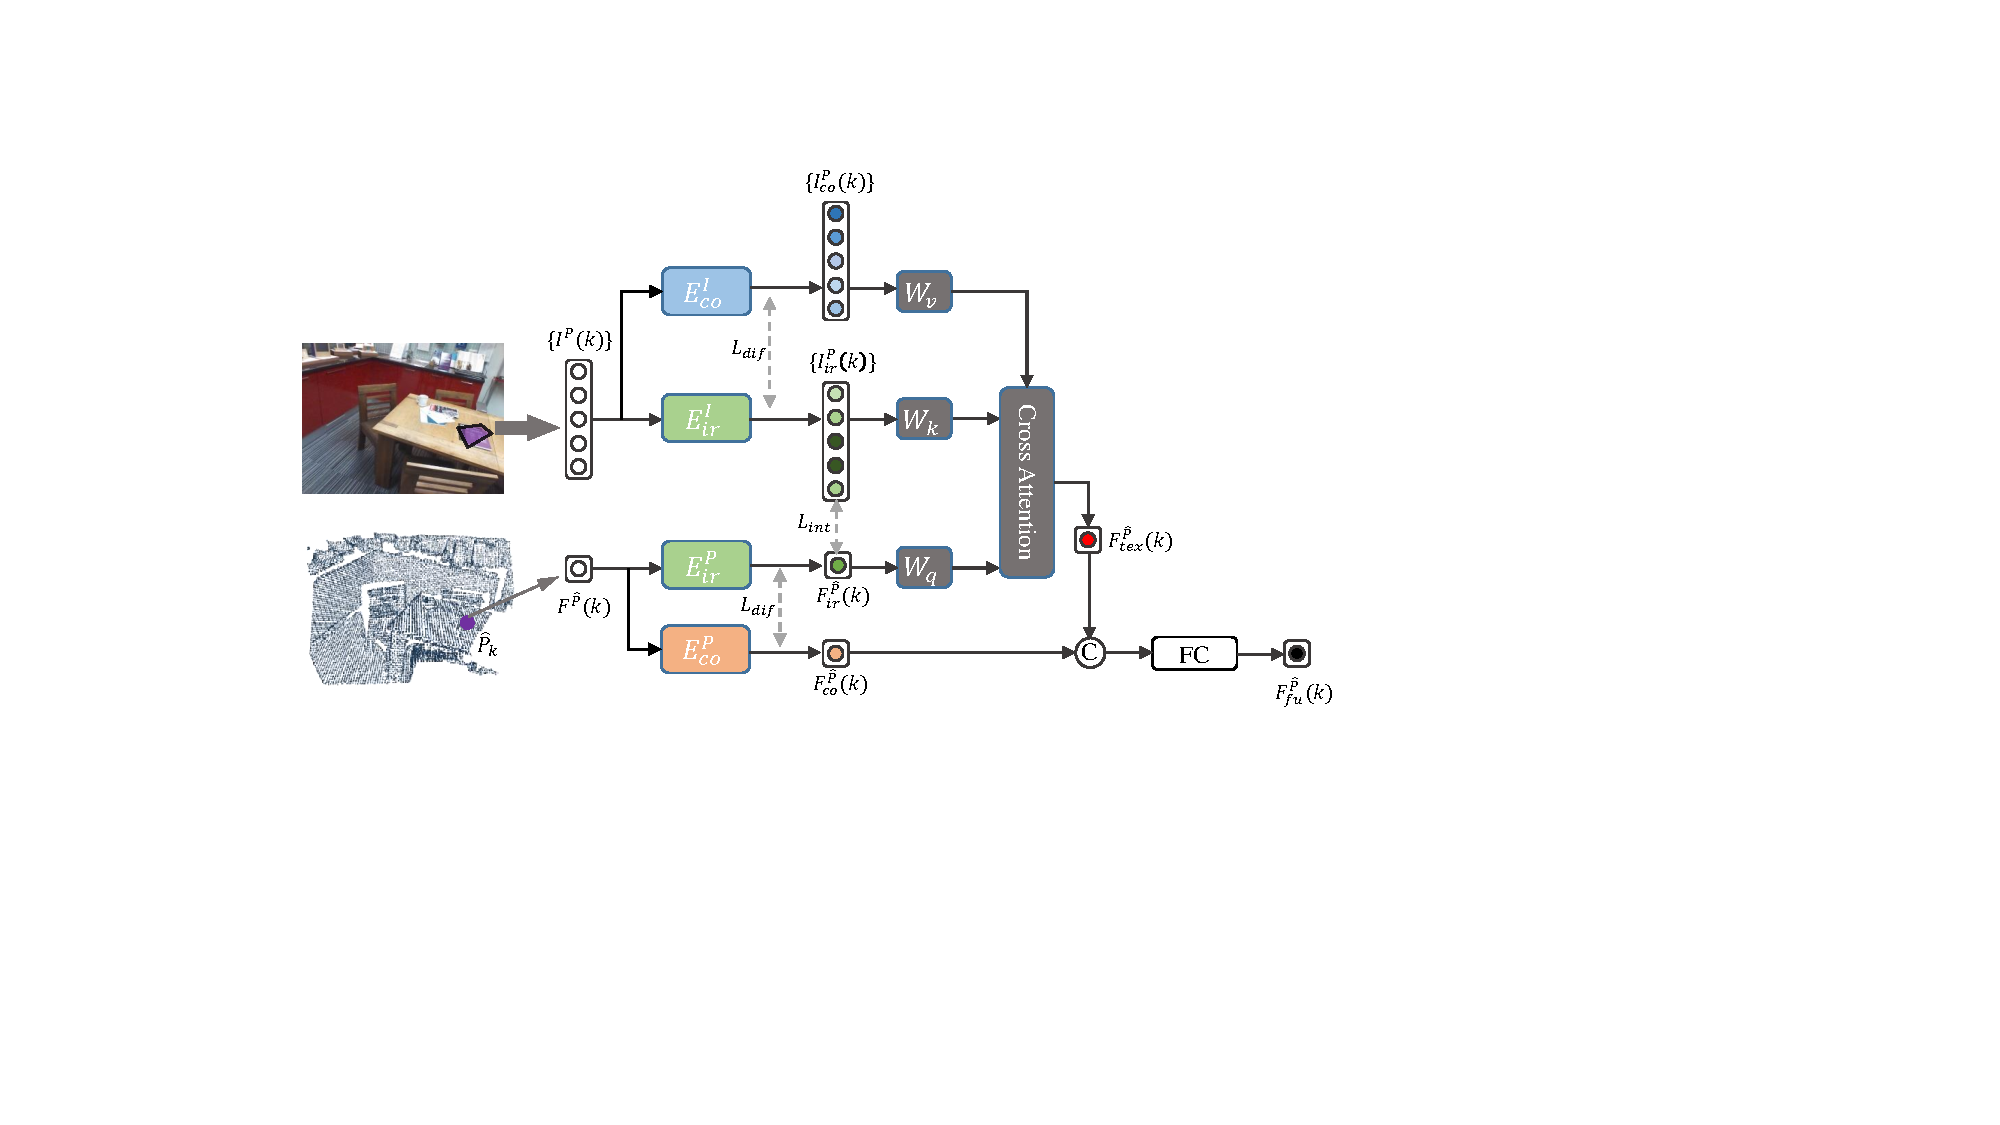
\includegraphics[width = \textwidth]{my/figure/4-3.pdf}
        % \captionsetup{margin = {1.6cm,1.6cm}}
        \bicaption[\xiaosi 特征融合模块流程图]{\wuhao 特征融合模块流程图}{\wuhao Flowchart of feature fusion module}
        \label{fig:4-3}
    \end{figure}
    \vspace{-0.35cm}

    类似的,利用解耦器$\mathbf{E}^{I}_{ir}$和解耦器$\mathbf{E}^{I}_{co}$将$\{\mathbf{I}^{\mathcal{P}}(k)\}$解码为图像模态无关特征$\{\mathbf{I}^{\mathcal{P}}_{ir}(k)\}$和图像模态相关特征$\{\mathbf{I}^{\mathcal{P}}_{co}(k)\}$。可用公式(4-2)表示上述解码过程:
    \begin{equation}
        \left\{
        \begin{aligned}
            \{{\mathbf{I}^{\mathcal{P}}_{ir}(k)}\} = \mathbf{E}^{I}_{ir}(\{\mathbf{I}^{\mathcal{P}}(k)\}) \\
            \{{\mathbf{I}^{\mathcal{P}}_{co}(k)}\} = \mathbf{E}^{I}_{co}(\{\mathbf{I}^{\mathcal{P}}(k)\}) \\
            \mathbf{F}^{\hat{\mathcal{P}}}_{ir}(k) = \mathbf{E}^{P}_{ir}(\mathbf{F}^{\hat{\mathcal{P}}}(k)) \\
            \mathbf{F}^{\hat{\mathcal{P}}}_{co}(k) = \mathbf{E}^{P}_{co}(\mathbf{F}^{\hat{\mathcal{P}}}(k))
        \end{aligned} \right.
    \end{equation}

    提取模态无关特征的目的在于提取潜在的公共特征,从而缩小不同模态之间的域间隙。在得到$\mathbf{F}^{\hat{\mathcal{P}}}_{ir}(k)$和$\{\mathbf{I}^{\mathcal{P}}_{ir}(k)\}$之后,本模块利用可学习矩阵$\mathbf{W}_q$和$\mathbf{W}_k$分别对两种模态无关特征进行映射后计算得到第$k$超点与它所对应图像区域像素的相似度矩阵$\mathbf{S}^{P}(k)$。具体来说,第$k$个超点与它的第$i$个像素的相似度分数$s^{P}(k,i)$可由公式(4-3)计算:
    \begin{equation}
        \begin{aligned}
            \mathbf{s}^{P}(k,i) = 
            (\mathbf{W}_q \mathbf{F}^{\hat{\mathcal{P}}}_{ir}(k))
            (\mathbf{W}_k \mathbf{I}^{\mathcal{P}}_{ir}(k,i))^\mathrm{T}
        \end{aligned}
    \end{equation}
    
    式中,$\mathbf{I}^{\mathcal{P}}_{ir}(k,i)$是第$k$个超点的第$i$个对应像素特征$\mathbf{I}^{\mathcal{P}}(k,i)$在模态无关子空间中的投影。随后$\{\mathbf{I}^{\mathcal{P}}_{co}(k)\}$经过$\mathbf{W}_v$的映射并结合相似度矩阵进行加权求和可以得到第$k$超点的纹理特征$\mathbf{F}^{\mathcal{P}}_{tex}(k)$:
    \begin{equation}
        \begin{aligned}
            \mathbf{F}^{\mathcal{P}}_{tex}(k) = \sum_i \mathbf{s}^{P}(k,i) \mathbf{I}^{\mathcal{P}}_{co}(k,i)
        \end{aligned}
    \end{equation}
    式中,$\mathbf{I}^{\mathcal{P}}_{co}(k,i)$第$k$个超点的第$i$个对应像素特征$\mathbf{I}^{\mathcal{P}}(k,i)$在模态相关子空间中的投影。相比于直接利用$\mathbf{F}^{\hat{\mathcal{P}}}(k)$与$\{\mathbf{I}^{\mathcal{P}}(k)\}$进行特征融合,上述方法由于在特征无关子空间中进行不同模态特征的查询,缩小了两种模态的域间隙减少了独有信息的影响。同理可以得到源点云中所有超点的纹理特征$\mathbf{F}^{\hat{\mathcal{P}}}_{tex}$。

    在得到超点的纹理特征$\mathbf{F}^{\mathcal{P}}_{tex}$之后,本文再将超点的模态相关特征$\mathbf{F}^{\hat{\mathcal{P}}}_{co}$与之在通道维度上拼接,并将其送入最后的映射层完成特征融合。可由公式(4-5)表示:
    \begin{equation}
        \mathbf{F}^{\hat{\mathcal{P}}}_{fu} = f(\mathbf{F}^{\hat{\mathcal{P}}}_{co} \oplus \mathbf{F}^{\hat{\mathcal{P}}}_{tex})
    \end{equation}
    式中,$f(\cdot)$表示映射层,由全连接层和激活函数构成。将$\mathbf{F}^{\mathcal{P}}_{tex}$和$\mathbf{F}^{\hat{\mathcal{P}}}_{co}$融合主要是为了避免两种模态独有信息的丢失。同理可以得到目标点云融合后的超点特征$\mathbf{F}^{\hat{\mathcal{Q}}}_{fu}$。

    \subsection{损失函数}
    为了使融合模块中的四个解耦器$\mathbf{E}^{I}_{ir}$、$\mathbf{E}^{I}_{co}$、$\mathbf{E}^{P}_{ir}$和$\mathbf{E}^{P}_{co}$达到设计要求。本文利用差异损失$\mathcal{L}_{dif}$和三元组损失$\mathcal{L}_{int}$分别监督同一模态特征和不同模态特征。
    \subsubsection{差异损失}
    差异损失主要是为了使同一模态的两种解码器能够捕获输入特征的不同方面的信息。通过解耦模态相关特征和模态无关特征之间存在一个正交约束。具体的,对于第$k$个超点的第$i$个像素特征在两个子空间的投影$\mathbf{I}^{\mathcal{P}}_{ir}(k,i)$和$\mathbf{I}^{\mathcal{P}}_{co}(k,i)$来说,理论上它们存在公式(4-6)的正交约束:
    \begin{equation}
        \Vert \mathbf{I}^{\mathcal{P}}_{ir}(k,i) (\mathbf{I}^{\mathcal{P}}_{co}(k,i))^\mathrm{T} \Vert^2_F = 0
    \end{equation}
    式中,$\Vert \cdot \Vert^2_F$表示Feobenius范数的平方。同时,这种约束对于第$k$个超点在两个子空间中的投影依旧成立。为此,本文使用的差异损失$\mathcal{L}_{dif}$如公式(4-7)所示:
    \begin{equation}
        \mathcal{L}_{dif} = 
        \sum_k (\Vert \mathbf{F}^{\hat{\mathcal{P}}}_{ir}(k) (\mathbf{F}^{\hat{\mathcal{P}}}_{co}(k))^\mathrm{T} \Vert^2_F) + 
        \sum_{k,i} (\Vert \mathbf{I}^{\mathcal{P}}_{ir}(k,i) (\mathbf{I}^{\mathcal{P}}_{co}(k,i))^\mathrm{T} \Vert^2_F)
    \end{equation}

    \subsubsection{三元组损失}
    模态无关特征指的是同一事物的结构纹理等信息不随表示形式的变化而变化的那部分。将点云和图像两种模态的特征同时投影至模态无关子空间中,得到每个模态自身的模态无关向量。模态间的损失函数的作用就是让不同模态的模态无关向量更加相似,这有助于通过一种模态特征查询另一种模态特征。本方法使用三元组损失函数监督两种模态在模态无关子空间中的投影。三元组损失在拉近锚点和正样本之间距离的同时,增加锚点与负样本之间的距离。具体而言,任一超点的模态无关特征和它对应像素的模态无关特征之间的距离要小于它与其他像素之间的特征距离;同时,对应像素集合中的特征距离要小于与其他像素之间的特征距离。因此,本文使用的三元损失$\mathcal{L}_{int}$如公式(4-8)所示:
    \begin{equation}
        \begin{aligned}
        \mathcal{L}_{int} = 
        \sum_{k,x} max(\lambda - 
        d(\mathbf{F}^{\hat{\mathcal{P}}}_{ir}(k), \{\mathbf{I}^{\mathcal{P}}_{ir}(k)\}) + 
        d(\mathbf{F}^{\hat{\mathcal{P}}}_{ir}(k), \{\mathbf{I}^{\mathcal{P}}_{ir}(x)\}))
        \\
        +\sum_{k,x} max(\lambda - 
        d(\mathbf{F}^{\hat{\mathcal{P}}}_{ir}(k), \{\mathbf{I}^{\mathcal{P}}_{ir}(k)\}) + 
        d(\mathbf{F}^{\hat{\mathcal{P}}}_{ir}(x), \{\mathbf{I}^{\mathcal{P}}_{ir}(k)\}))
        \end{aligned}
    \end{equation}
    式中,$\lambda$用于控制正负样本之间的距离;$(\mathbf{F}^{\hat{\mathcal{P}}}_{ir}(k), {\mathbf{I}^{\mathcal{P}}_{ir}(k)})$对应三元损失中的正样本对;$(\mathbf{F}^{\hat{\mathcal{P}}}_{ir}(k), {\mathbf{I}^{\mathcal{P}}_{ir}(x)})$和$(\mathbf{F}^{\hat{\mathcal{P}}}_{ir}(x), {\mathbf{I}^{\mathcal{P}}_{ir}(k)})$对应三元函数的负样本对。$d(\mathbf{F}^{\hat{\mathcal{P}}}_{ir}(x), {\mathbf{I}^{\mathcal{P}}_{ir}(y)})$表示超点$\mathcal{P}_x$与超点$\mathcal{P}_y$所对应像素集之间的距离和,由公式(4-9)定义:
    \begin{equation}
        \begin{aligned}
        d(\mathbf{F}^{\hat{\mathcal{P}}}_{ir}(x), \{\mathbf{I}^{\mathcal{P}}_{ir}(y)\}) =
        \sum_i -\Vert max(0, \mathbf{F}^{\hat{\mathcal{P}}}_{ir}(x) - \mathbf{I}^{\mathcal{P}}_{ir}(y,i)) \Vert^2
        \end{aligned}
    \end{equation}

    \section{实验结果与分析}
    \subsection{数据集预处理}
    本章采用的数据集3DMatch和3DLoMatch与第三章略有差别。在上一章所用数据集的基础上本章为每个点云配对了RGB图像数据。RGB图像数据来自于最原始的3DMatch数据集,每50张图像合成一个点云数据。为了减少时间花销,本方法没有使用全部的50张图片而是选择第一张图片用于多模态融合。同时,本方法记录了第一帧图片的相机位姿和相机内参并加入了数据集,以保证本章中的对其模块能够正常使用。至此,整个数据集的预处理完成,整个数据集由点云、图像和相机的内参外参矩阵组成。
    \subsection{3DMatch和3DLoMatch实验}
    在本节中,本文对多模态融合的点云配准任务在3DMatch和3DLoMatch上进行了实验分析。实验表明,通过融合图像特征本方法的点云配准方法能够达到较好水平。
    % 在表\ref{tab:4-1-1}、表\ref{tab:4-1-2}和表\ref{tab:4-1-3}中分别记录了本方法在3DMatch和3DLoMatch数据集上采样数为5000、2500、1000、500和250时的内点率、特征召回率和配准召回率的实验对比。
    如表\ref{tab:4-1-1}所示,本方法在内点率上远高于其他方法。尤其当采样数为250时,在3DMatch和3DLoMatch上比CoFiNet分别高了32.4\%和30.2\%。这表明本方法能够在相同情况下比其他方法能够更加有效的找到正确的点对应。\par
    \begin{table}[htp]
    \renewcommand{\arraystretch}{1}
    \centering
    \bicaption[\xiaosi 第四章方法与先进方法的内点率]{\wuhao 本方法与先进方法的内点率和匹配召回率的比较}{\wuhao Comparison of Inlier Ratio with advanced methods}\label{tab:4-1-1}
    \wuhao

    \begin{tabular}{lcccccccccc}
    \toprule[1.5pt]
    \multicolumn{1}{c}{\multirow{3}{*}{\songti\wuhao Sample}} 
    & \multicolumn{5}{c}{\songti\wuhao 3DMatch}
    & \multicolumn{5}{c}{\songti\wuhao 3DLoMatch}
    \\\multicolumn{1}{c}{}
    &\songti\wuhao 5000 &\songti\wuhao 2500 &\songti\wuhao 1000 &\songti\wuhao500 
    &\multicolumn{1}{c}{\songti\wuhao 250}           
    &\songti\wuhao 5000 &\songti\wuhao 2500 &\songti\wuhao 1000 &\songti\wuhao500 
    &\songti\wuhao 250

    \\ \hline

    \multicolumn{1}{c}{\wuhao PerfectMatch}
    & 36.0          & 32.5          & 26.4          & 21.5          & \multicolumn{1}{c}{16.4}          & 11.4          & 10.1          & 8.1           & 6.4           & 4.8
    \\
    \multicolumn{1}{c}{\wuhao FCGF}
    & 56.8          & 54.1          & 48.7          & 42.5          & \multicolumn{1}{c}{34.1}          & 21.4          & 20.0          & 17.2          & 14.8          & 11.6
    \\
    \multicolumn{1}{c}{\wuhao D3Feat}
    & 39.0          & 38.8          & 40.4          & 41.5          & \multicolumn{1}{c}{41.8}          & 13.2          & 13.1          & 14.0          & 14.6          & 15.0
    \\
    \multicolumn{1}{c}{\wuhao SpinNet}
    & 47.5          & 44.7          & 39.4          & 33.9          & \multicolumn{1}{c}{27.6}          & 20.5          & 19.0          & 16.3          & 13.8          & 11.1
    \\
    \multicolumn{1}{c}{\wuhao Predator}
    & 58.0          & 58.4          & \ul{57.1}    & \ul{54.1}    & \multicolumn{1}{c}{49.3}          & \ul{26.7}    & \ul{28.1}    & \ul{28.3}    & \ul{27.5}    & 25.8
    \\
    \multicolumn{1}{c}{\wuhao YOHO}
    & \ul{64.4}    & \ul{60.7}    & 55.7          & 46.4          & \multicolumn{1}{c}{41.2}          & 25.9          & 23.3          & 22.6          & 18.2          & 15.0
    \\
    \multicolumn{1}{c}{\wuhao CoFiNet}
    & 49.8          & 51.2          & 51.9          & 52.2          & \multicolumn{1}{c}{\ul{52.2}}    & 24.4          & 25.9          & 26.7          & 26.8          & \ul{26.9}
    \\

    \multicolumn{1}{c}{\wuhao Ours}
    & \textbf{71.9} & \textbf{78.5} & \textbf{83.0} & \textbf{84.8} & \multicolumn{1}{c}{\textbf{85.8}} & \textbf{41.4} & \textbf{47.0} & \textbf{52.9} & \textbf{55.5} & \textbf{57.1}
    
    \\ \bottomrule[1.5pt]
    \end{tabular}
\end{table}

    对于特征召回率而言,本方法虽然在3DMatch上的表现一般,在采样数为5000、2500和250时分别比最优模型低了0.2\%、0.3\%和0.4\%。但是如表\ref{tab:4-1-2}所示,本方法在3DLoMatch的表现都达到了最优性能,分别比次优模型高了4.5\%、4.4\%、4.1\%、4.3\%和4.2\%。这表明本方法相比于其他方法能够更好的在低重叠率情况下工作,能够使源点云和目标点云之间的点对应更多,从而达到RANSAC算法发挥最用的最低要求。\par
    \begin{table}[htbp]
    \renewcommand{\arraystretch}{1}
    \centering
    \bicaption[\xiaosi 第四章方法与先进方法的匹配召回率的比较]{\wuhao 本方法与先进方法的匹配召回率的比较}{\wuhao Comparison of Feature Matching Recall with advanced methods}\label{tab:4-1-2}
    \wuhao

    \begin{tabular}{lcccccccccc}
    \toprule[1.5pt]
    \multicolumn{1}{c}{\multirow{3}{*}{\songti\wuhao Sample}} 
    & \multicolumn{5}{c}{\songti\wuhao 3DMatch}
    & \multicolumn{5}{c}{\songti\wuhao 3DLoMatch}
    \\\multicolumn{1}{c}{}
    &\songti\wuhao 5000 &\songti\wuhao 2500 &\songti\wuhao 1000 &\songti\wuhao500 
    &\multicolumn{1}{c}{\songti\wuhao 250}           
    &\songti\wuhao 5000 &\songti\wuhao 2500 &\songti\wuhao 1000 &\songti\wuhao500 
    &\songti\wuhao 250

    \\ \hline

    \multicolumn{1}{c}{\wuhao PerfectMatch}
    & 95.0          & 94.3          & 92.9          & 90.1          & \multicolumn{1}{c}{82.9}          & 63.6          & 61.7          & 53.6          & 45.2          & 34.2
    \\
    \multicolumn{1}{c}{\wuhao FCGF}
    & 97.4          & 97.3          & 97.0          & 96.7          & \multicolumn{1}{c}{96.6}          & 76.6          & 75.4          & 74.2          & 71.7          & 67.3
    \\
    \multicolumn{1}{c}{\wuhao D3Feat}
    & 95.6          & 95.4          & 94.5          & 94.1          & \multicolumn{1}{c}{93.1}          & 67.3          & 66.7          & 67.0          & 66.7          & 66.5
    \\
    \multicolumn{1}{c}{\wuhao SpinNet}
    & 97.6          & 97.2          & 96.8          & 95.5          & \multicolumn{1}{c}{94.3}          & 75.3          & 74.9          & 72.5          & 70.0          & 63.6
    \\
    \multicolumn{1}{c}{\wuhao Predator}
    & 96.6          & 96.6          & 96.5          & 96.3          & \multicolumn{1}{c}{96.5}          & 78.6          & 77.4          & 76.3          & 75.7          & 75.3
    \\
    \multicolumn{1}{c}{\wuhao YOHO}
    & \textbf{98.2} & 97.6          & 97.5    & \ul{97.7}    & \multicolumn{1}{c}{96.0}          & 79.4          & 78.1          & 76.3          & 73.8          & 69.1
    \\
    \multicolumn{1}{c}{\wuhao CoFiNet}
    & \ul{98.1}    & \textbf{98.3} & \ul{98.1} & \textbf{98.2} & \multicolumn{1}{c}{\textbf{98.3}} & \ul{83.1}    & \ul{83.5}    & \ul{83.3}    & \ul{83.1}    & \ul{82.6}
    \\
    \multicolumn{1}{c}{\wuhao Ours}
    & 98.0          & \ul{98.0}    & \textbf{98.4} & \textbf{98.2} & \multicolumn{1}{c}{\textbf{98.3}}    & \textbf{87.6} & \textbf{87.9} & \textbf{87.4} & \textbf{87.4} & \textbf{86.8}
    
    \\ \bottomrule[1.5pt]
    \end{tabular}
\end{table}

    本方法进一步与各个先进方法在匹配召回率上做了对比。如表\ref{tab:4-1-3}所示,本方法在3DLoMatch和3DMatch数据集上的性能均达到了当前最优的性能。具体来说,在3DMatch上当采样数为5000、2500、1000、500和250时,本模型的新能分别比次优模型高了0.2\%、1\%、0.1\%、1.4\%和2.3\%;在3DLoMatch上则分别高出了2.5\%、3.3\%、6\%、6.4\%和7.5\%。这表明本方法生成的点对应关系能够有效的实现点云间的配准。同时可以注意到,本方法的性能的变化幅度远远低于其他方法,其他模型的性能随着采样数的减少有明显下降。这表明本方法能够有效提取空间一致性的点对应,即使在低重叠率的情况下,也能够通过少数高置信度的点对应恢复点云间的变换矩阵。这也表明通过融合图像特征,本模型受到的噪声影响更小,模型更加稳定。\par
    \begin{table}[ht]
    \renewcommand{\arraystretch}{1}
    \centering
    \bicaption[\xiaosi 本方法与先进方法的配准召回率的比较]{\wuhao 本方法与先进方法的配准召回率的比较}{\wuhao Comparison of registration recall rates of this method with advanced methods}\label{tab:4-1-3}
    \wuhao
    
    \begin{tabular}{lcccccccccc}
    \toprule[1.5pt]
    \multicolumn{1}{c}{\multirow{3}{*}{\songti\wuhao Sample}} 
    & \multicolumn{5}{c}{3DMatch}
    & \multicolumn{5}{c}{3DLoMatch}
    \\ \multicolumn{1}{c}{}
    &\songti\wuhao 5000 &\songti\wuhao 2500 &\songti\wuhao 1000 &\songti\wuhao500 
    &\multicolumn{1}{c}{\songti\wuhao 250}           
    &\songti\wuhao 5000 &\songti\wuhao 2500 &\songti\wuhao 1000 &\songti\wuhao500 
    &\songti\wuhao 250    

    \\ \hline

    \multicolumn{1}{l}{\wuhao PerfectMatch}
    & 78.4          & 76.2          & 71.4          & 67.6          & \multicolumn{1}{c}{50.8}          & 33.0          & 29.0          & 23.3          & 17.0          & 11.0
    \\
    \multicolumn{1}{l}{\wuhao FCGF}
    & 85.1          & 84.7          & 83.3          & 81.6          & \multicolumn{1}{c}{71.4}          & 40.1          & 41.7          & 38.2          & 35.4          & 26.8
    \\
    \multicolumn{1}{l}{\wuhao D3Feat}
    & 81.6          & 84.5          & 83.4          & 82.4          & \multicolumn{1}{c}{77.9}          & 37.2          & 42.7          & 46.9          & 43.8          & 39.1
    \\
    \multicolumn{1}{l}{\wuhao SpinNet}
    & 88.6          & 86.6          & 85.5          & 83.5          & \multicolumn{1}{c}{70.2}          & 59.8          & 54.9          & 48.3          & 39.8          & 26.8
    \\
    \multicolumn{1}{l}{\wuhao Predator}
    & 89.0          & 89.9    & \ul{90.6} & 88.5          & \multicolumn{1}{c}{86.6}          & 59.8          & 61.2          & 62.4          & 60.8          & 58.1
    \\
    \multicolumn{1}{l}{\wuhao YOHO}
    & \ul{90.8} & \ul{90.3} & 89.1          & \ul{88.6} & \multicolumn{1}{c}{84.5}          & 65.2          & 65.5          & 63.2          & 56.5          & 48.0
    \\
    \multicolumn{1}{l}{\wuhao CoFiNet}
    & 89.3          & 88.9    & 88.4          & 87.4          & \multicolumn{1}{c}{\ul{87.0}}    & \ul{67.5}    & \ul{66.2}    & \ul{64.2}    & \ul{63.1}    & \ul{61.0}
    \\
    \multicolumn{1}{l}{\wuhao Ours}
    & \textbf{91.0}    &\textbf{91.3}          & \textbf{90.7}    & \textbf{90.0}    & \multicolumn{1}{c}{\textbf{89.3}} & \textbf{70.0} & \textbf{69.5} & \textbf{70.2} & \textbf{69.5} & \textbf{68.5}
    \\
    \bottomrule[1.5pt]
    \end{tabular}
\end{table}

    本章同样使用加权奇异值分解法和局部到全局变换估计两种算法估计变换矩阵,表\ref{tab:4-3}的实验结果进一步验证了上述表述。本实验首先使用加权奇异值分解算法求解变换矩阵,其他模型要么不能达到合理的结果,要么性能严重下降。比如CoFiNet模型使用加权奇异值分解进行变换估计时比基于RANSAC的变换估计性能在3DMatch和3DLoMatch上分别下降了24.7\%和49.5\%。相比之下,本方法在3DMatch上的配准召回率达到了84.7\%仅比利用RANSAC得到的结果下降了5.3\%。在3DLoMatch上虽然性能下降了14.1\%,但是也接近了Predator方法性能。这得益于本方法能够有效找到可靠和分布良好的超点对应。当使用局部到全局配准进行变换估计时,本方法在3DMatch上的配准召回率达到90.6\%,3DLoMatch的配准召回率达到73.1\%,基本达到了其他模型使用RANSAC的结果。\par
    \begin{table}[ht]
    \renewcommand{\arraystretch}{1}
    \centering
    \bicaption[\xiaosi 在3DMatch和3DLoMatch上使用不同姿态估计器的配准结果]{\wuhao 在3DMatch和3DLoMatch上使用不同姿态估计器的配准结果}{\wuhao Registration results with different pose estimators on 3DMatch and 3DLoMatch}\label{tab:4-3}
    \wuhao

    \begin{tabular}{lccccccc}
    \toprule[1.5pt]
    \multirow{2}{*}{\songti\wuhao Model} 
    & \multirow{2}{*}{\songti\wuhao Estimator} 
    & \multirow{2}{*}{\songti\wuhao Sample} 
    & \multicolumn{2}{c}{\songti\wuhao RR(\%)}   
    & \multicolumn{3}{c}{\songti\wuhao Times(s)} \\
    
    & &
    &{\songti\wuhao 3DMatch} &{\songti\wuhao 3DLoMatch}
    &{\songti\wuhao Model}   &{\songti\wuhao Pose}    &{\songti\wuhao Total}
    
    \\ \hline
    {\songti\wuhao FCGF} &{\songti\wuhao RANSAC-50k} & 5000
    & 85.1          & 40.1          & 0.098   & 9.015   & 9.113   
    \\
    % {\songti\wuhao D3Feat} &{\songti\wuhao RANSAC-50k} & 5000
    % & 81.6          & 37.2          & 0.055   & 8.217   & 8.272   
    % \\
    {\songti\wuhao Predator} &{\songti\wuhao RANSAC-50k} & 5000
    & 89.0          & 59.8          & 0.079   & 15.434  & 15.513  
    \\
    {\songti\wuhao CoFiNet} &{\songti\wuhao RANSAC-50k} & 5000
    & \uline{89.3}    & \uline{67.5}    & 0.259   & 5.321   & 5.580   
    \\
    {\songti\wuhao Ours} &{\songti\wuhao RANSAC-50k} & 5000
    & \textbf{91.0} & \textbf{70.0} & 0.141   & 4.215   & 4.356   
    
    \\ \hline
    {\songti\wuhao FCGF} &{\songti\wuhao weighted SVD} & 250
    & 42.1          & 3.9           & 0.098   & 0.008   & 0.106   
    \\
    % {\songti\wuhao D3Feat} &{\songti\wuhao weighted SVD} & 250
    % & 37.4          & 2.8           & 0.055   & 0.008   & 0.063   
    % \\
    {\songti\wuhao Predator} &{\songti\wuhao weighted SVD} & 250
    & 50.0          & 6.4           & 0.079   & 0.010   & 0.089   
    \\
    {\songti\wuhao CoFiNet} &{\songti\wuhao weighted SVD} & 250
    & \uline{64.6}    & \uline{21.6}    & 0.259   & 0.004   & 0.263   
    \\
    {\songti\wuhao Ours} &{\songti\wuhao weighted SVD} & 250
    & \textbf{84.7} & \textbf{55.9} & 0.141   & 0.004   & 0.145   
    \\ \hline
    {\songti\wuhao CoFiNet} &{\songti\wuhao LGR} & all
    & \uline{87.6}    & \uline{64.8}    & 0.259   & 0.242   & 0.501   
    \\
    {\songti\wuhao Ours} &{\songti\wuhao LGR} & all
    & \textbf{90.6} & \textbf{73.1} & 0.141   & 0.317   & 0.458   
    \\ 
    \bottomrule[1.5pt]
    \end{tabular}
\end{table}
    
    本文进一步在3DMatch和3DLoMatch数据集上测试了相对旋转误差和相对平移误差。如\ref{tab:4-4}所示,本方法相比于其他方法有明显优势,在3DMatch和3DLoMatch中都获得了最低的相对旋转误差和相对平移误差。在3DMatch上,本方法的相对旋转误差和相对平移误差分别比次优模型的性能低了
    0.138$^\circ$和0.001cm。尤其在3DLoMatch上,本方法的相对旋转误差比次优的Predator小了0.202$^\circ$。该实验结果表明通过将图像中的纹理信息和点云的结构信息相融合,能够提高点对应的数量和质量,能够使模型在配得“多”的同时配得“好”,这也从侧面验证了本方法融合方式的有效性。
    \begin{table}[h]
    \renewcommand{\arraystretch}{1}
    \centering

    \setlength{\tabcolsep}{7mm}{
    \bicaption[\xiaosi 3DMatch和3DLoMatch的相对平移误差和相对旋转误差比较]{\wuhao 3DMatch和3DLoMatch的相对平移误差和相对旋转误差比较}{\wuhao Comparison of RRE and RTE on 3DMatch and 3DLoMatch}\label{tab:4-4}
    \wuhao

    \begin{tabular}{lcccc}
        \toprule[1.5pt]
    \multirow{2}{*}{Model} & \multicolumn{2}{c}{3DMatch} & \multicolumn{2}{c}{3DLoMatch}
    \\
    &{\songti\wuhao RRE($^\circ$)} &{\songti\wuhao RTE(cm)}
    &{\songti\wuhao RRE($^\circ$)} &{\songti\wuhao RTE(cm)}       
    \\ \hline
    {\songti\wuhao FCGF}
    & \ul{1.949}     & 0.066          & 3.146          & 0.100          \\
    {\songti\wuhao D3Feat}
    & 2.161          & 0.067          & 3.361          & 0.103          \\
    {\songti\wuhao Predator}
    & 2.029          & \ul{0.064}    & \ul{3.048}    & \ul{0.093}    \\
    {\songti\wuhao CoFiNet}
    & 2.002          & \ul{0.064}    & 3.271          & \textbf{0.090} \\
    {\songti\wuhao Ours}
    & \textbf{1.811} & \textbf{0.063} & \textbf{2.846} & \textbf{0.090} \\
    \bottomrule[1.5pt]
    \end{tabular}
    }
\end{table}

    图\ref{fig:4-4}中展示了当前方法和CoFiNet方法两种方法配准结果的可视化。如图\ref{fig:4-4}所示,本方法不仅在重叠率高于30\%时实现配准,而且在重叠率低至14\%时也能准确配准点云。
    \vspace{-0.1cm}
    \begin{figure}[H]
        \centering
        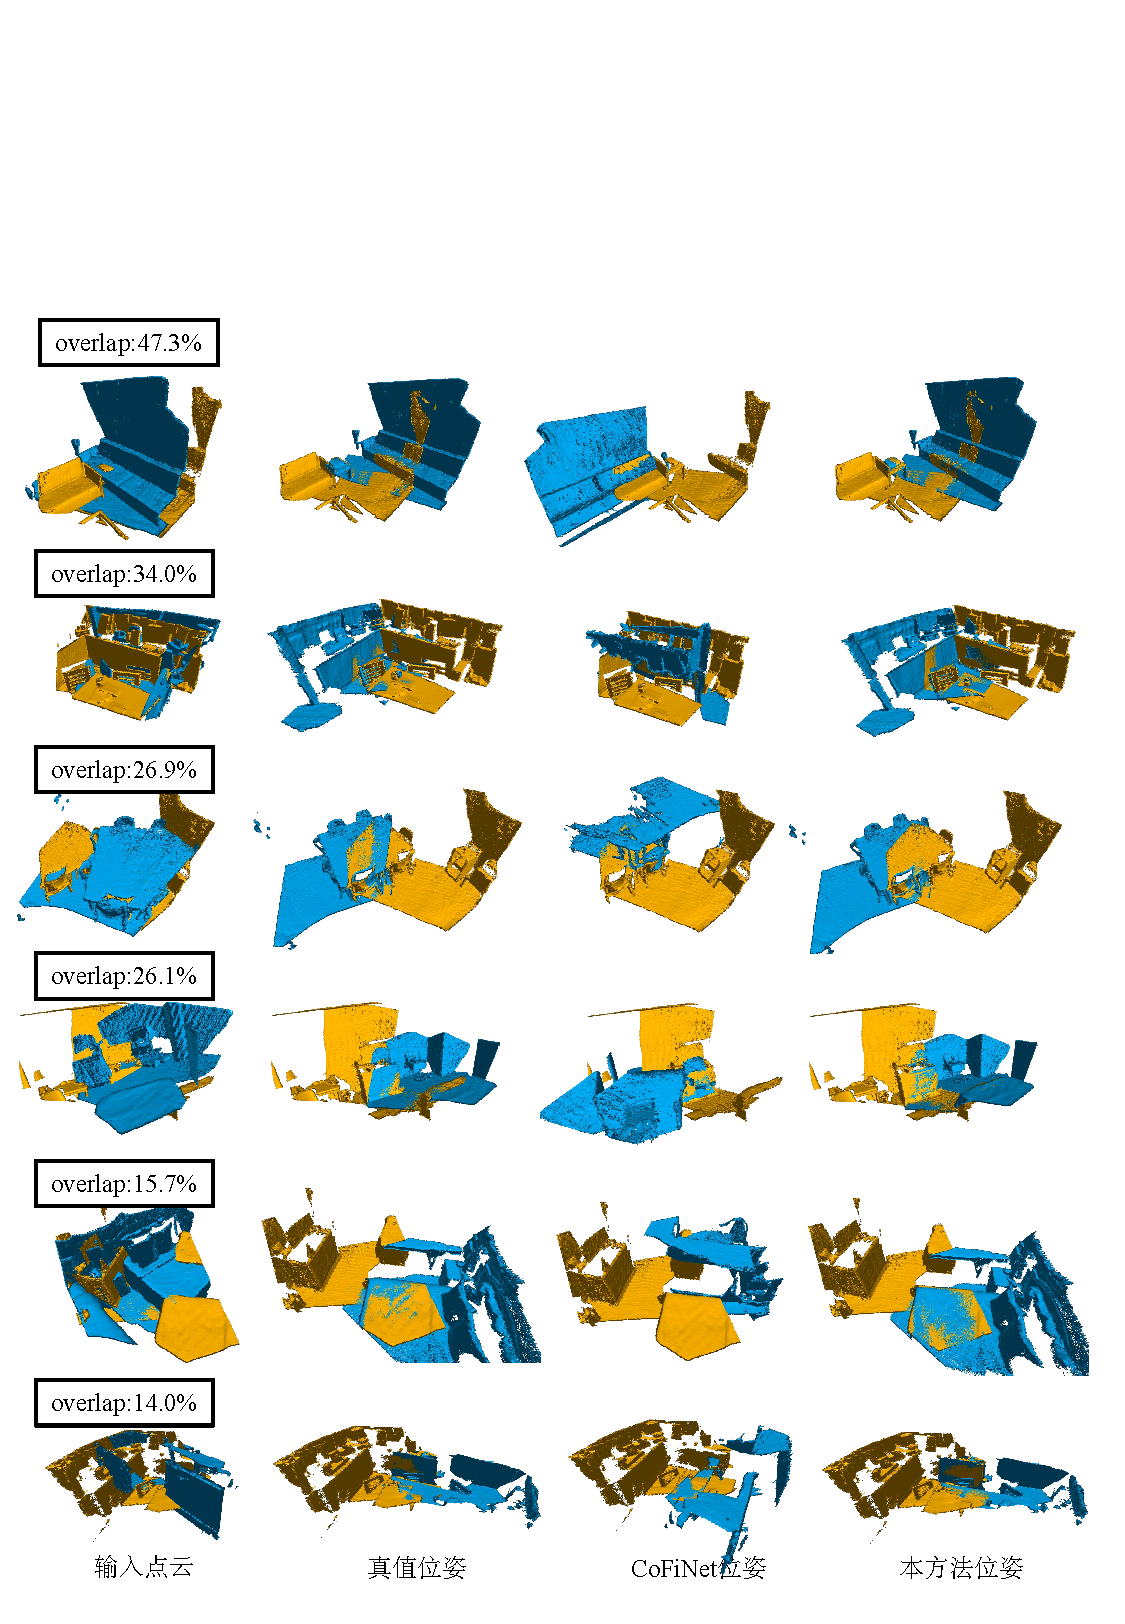
\includegraphics[width = \textwidth]{my/figure/4-4.pdf}
        \captionsetup{margin = {1.6cm,1.6cm}}
        \bicaption[\xiaosi 配准结果可视化]{\wuhao 配准结果可视化
        % 。(a) 输入点云;(b) 真实位姿;(c) CoFiNet位姿;(d) 本方法位姿
        }
        {\wuhao Visualization of registration results
        % . (a) Input; (b) Ground truth; (c) CoFiNet Pose; (d) Our Pose
        }
        \label{fig:4-4}
    \end{figure}
    \vspace{-0.35cm}

    \subsection{消融实验}
    本文提出的基于多模态融合的锚点定位点云配准方法为解决点云配准提供了一种新的思路,为了验证对齐模块和融合模块的有效性,本节将对这两个模块进行消融实验。

    \subsubsection{对齐模块的效果}表\ref{tab:4-5}展示了对齐模块的对本点云配准框架的作用,实验结果显示了超点匹配率、特征召回率、内点率和匹配召回率四个性能指标。从表\ref{tab:4-5}可以看出,在使用对齐模块之后所有的性能指标都得到了有效提高。这说明在多模态特征融合之前进行模态间的数据对齐,寻找点云中的点和图像中的像素的对应有助于更好的特征融合。
    \begin{table}[H]
    \renewcommand{\arraystretch}{1}
    \centering
    \bicaption[\xiaosi 对齐模块消融实验]{\wuhao 对齐模块消融实验}{\wuhao Ablation experiments of alignment module}\label{tab:4-5}
    \wuhao

    \begin{tabular}{lcccccccc}
    \toprule[1.5pt]
    \multicolumn{1}{c}{\multirow{2}{*}{Model}}
    & \multicolumn{4}{c}{3DMatch}
    & \multicolumn{4}{c}{3DLoMatch}
    \\ \multicolumn{1}{c}{}
    
    & PIR   & FMR   & IR   & RR   & PIR   & FMR   & IR    & RR
    \\ \hline
    w/o Alignment
    & 83.4  & 98.0  & 68.8 & 89.0 & 53.1  & 85.6  & 42.4  & 71.8  \\
    Ours
    & 85.4  & 98.0  & 70.2 & 90.6 & 51.4  & 87.6  & 41.2  & 73.1  \\
    \bottomrule[1.5pt]
    \end{tabular}
\end{table}

    \subsubsection{融合模块的效果}在特征融合过程中,与以往的特征融合方式不同,本方法在两个子空间将超点特征和它所对应的像素特征进行了融合,表\ref{tab:4-6}验证本融合方式的有效性。
    其中cFusion表示直接将点云特征与图像特征进行拼接,aFusion表示将点云和图像特征直接利用注意力进行融合,iFusion表示仅在模态无关子空间进行特征融合。
    \begin{table}[htp]
    \renewcommand{\arraystretch}{1}
    \centering
    \bicaption[\xiaosi 融合模块消融实验]{\wuhao 融合模块消融实验}{\wuhao Ablation experiment of fusion module}\label{tab:4-6}
    \wuhao
    
    \begin{tabular}{lcccccccc}
    \toprule[1.5pt]
    \multicolumn{1}{c}{\multirow{2}{*}{\songti\wuhao Model}}
    & \multicolumn{4}{c}{\songti\wuhao 3DMatch}
    & \multicolumn{4}{c}{\songti\wuhao 3DLoMatch}
    \\ \multicolumn{1}{c}{}

    & PIR   & FMR   & IR   & RR   & PIR   & FMR   & IR    & RR    \\ \hline
    {\songti\wuhao cFusion}
    & 82.7  & 97.6  & 68.3 & 87.8 & 48.5  & 84.5  & 39.3  & 69.7  \\
    {\songti\wuhao aFusion}
    & 83.4  & 97.6  & 68.6 & 88.8 & 49.5  & 83.9  & 39.7  & 70.3  \\
    {\songti\wuhao iFusion}
    & 84.4  & 97.8  & 70.1 & 89.9 & 51.8  & 85.8  & 42.2  & 72.2  \\
    {\songti\wuhao Ours}
    & 85.4  & 98.0  & 70.2 & 90.6 & 51.4  & 87.6  & 41.2  & 73.1  \\
    \bottomrule[1.5pt]
    \end{tabular}
\end{table}
    可以看到融合模块能够有效提高各个阶段的实验性能。这说明通过将两种模态特征投影到模态无关子空间能够有效减少模态间的域差异,同时在模态相关子空间的特征融合能够减少信息的丢失。

    \section{本章小结}
    本章提出了一个基于多模态特征融合的锚点定位点云配准方法,在第三章的基于锚点几何嵌入点云配准基础框架中的锚点定位阶段引入了多模态融合辅助定位。一方面,受到3D目标检测同行多模态融合方法的启发,该方法利用一个对齐模块寻找点云的点与图像的像素之间的对应关系,实现像素到点的准确映射。另一方面,该方法加入模态相关与无关的特征学习,旨在在模态无关子空间中减少模态间特征差异,同时利用注意力机制融合不同模态的信息,并在模态相关子空间中融合最终特征防止信息丢失。实验表明,本章提出的方法对如何融合点云和图像信息并最终受益于点云配准方法提供了很好的解决思路,同时提高了点云配准的性能。相比于其他方法,本方法在多模态融合之前进行了模态间的对齐,提升了多模态融合的效果,取得了更好的点云配准任务的实验结果。

% 第5章
\chapter{总结与展望}
\thispagestyle{others}
\pagestyle{others}
\xiaosi

\section{主要结论}
随着科技的发展,计算机三维视觉与生产生活联系的越来越紧密,对点云的自动化处理成为了一个急切的需求。在自动驾驶的城市建图,在机器人领域的姿态估计以及虚拟现实中的三维建模,点云配准的应用广泛分布于各个生产生活环节。如何快速高效的实现各种复杂真实场景的点云配准是一项具有挑战和意义的研究。针对点云配准任务,本文提出了一种基于显著锚点的点云配准框架,它通过第三章的几何嵌入增加弱几何区域的特征差异性,通过引入第四章的多模态融合模块增加锚点的显著性。其中第四章可以看成是

针对第三章方法锚点选择的局限性做的进一步改进。两个方法都在真实场景的点云配准数据集上进行了实验和评估,实验结果表明本文提出的方法能够有效地在低重叠率得场景中,增强特征间的差异性提高相似区域重复模式的匹配成功率,并实现了当前点云配准方法的先进水平。两个方法得贡献如下:

(1)在基于显著锚点的点云配准方法中,通过提取显著锚点利用锚点与超点、超点与超点间的距离和角度等几何结构信息进行特征嵌入,增加了相似不重叠区域的差异性,能够有效提高超点匹配的内点率。该方法使用KPConv网络来提取点云局部区域的超点特征。利用一个锚点定位模块选取出若干保持一定几何结构的高置信度的锚点,并通过注意力机制对点云中的超点进行结构嵌入并寻找超点间的对应关系。最后,在经过将超点对应扩充为点对应之后,利用一个局部到全局的姿态估计得到最终的变换矩阵。

(2)在基于多模态特征融合的锚点定位点云配准方法中,通过融合点云和图像两种模态的信息,提高锚点选择的可靠性。该方法首先利用对其模块,将不同模态的两种数据进行对齐,寻找到点云到像素的对应关系。在多模态融合模块,将两种模态的特征分解为模态相关和模态无关的特征,并在模态无关子空间中缩小特征间的域间隙减少噪声干扰。并最终与模态相关的特征融合以减少信息的丢失形成最终的特征,实现锚点定位。

\section{研究展望}
本文提出了基于显著锚点几何嵌入的点云配准和基于多模态融合的锚点定位点云配准方法,虽然两个方法都在低重叠率的真实场景数据集上取得了不错的效果,但是仍然存在一些可以改进的地方。
本文的第三章提出了一种基于显著锚点几何嵌入的点云配准方法,其核心思想是通过多个保持一定几何机构的锚点缓解相似不重叠区域特征过度平滑问题。虽然该方法取得了一定的效果,但是仍然存在一些尚需改进的地方:(1)首先该方法虽然设计了一个锚点定位模块并利用迭代优化更新显著锚点,但是这种设计产生的锚点在某些场景中依然会失败,并导致最终的结果相较于一般方法较差。为此,需要设计一个更加鲁棒的锚点定位模块使得整体网络更加稳定,可以考虑设计一个损失函数来有效监督锚点对应。(2)其次在使用由粗到细的点云配准框架之后,整个网络的模型较大导致训练时间较长,如何有效轻量化模型是一个急需解决的问题。后续可以通过提高下采样倍率减少超点个数,进而减少几何嵌入过程的时间开销。

本文的第四章提出以一种基于多模态融合的锚点定位点云配准方法,其核心思想是通过将图像信息和点云信息进行特征融合提高锚点对应的准确性。该方案针对第三章框架做出一点改进并取得了一定效果,但也存在一些问题:(1)点云数据集中每个点云实际是由50张RGB-D图像合成,而文章中仅采取某一视角下的一张图片进行融合导致某些点在该视角下被遮挡找不到准确的图像信息,但是如果使用全部图像又会导致时间花销较大,故需要有效实验对图像数量对模态融合的影响进行分析。(2)在多模态融合模块中,将两种模态的特征投影到模态相关和模态无关的两个子空间并分别学习模态相关与无关的特征表示,后续工作可以重新设计更加适应点云和图像融合的损失函数对其进行监督以达到预设效果。同时在最终的融合过程中使用多头注意力机制完成,后续工作可以考虑使用其他的多模态融合方法。

如何增加点特征间的差异性缓解特征的过渡平滑是点云配准任务的关键,提出的两个方法都是借助锚点嵌入几何信息来提取最终特征。但是由于点云点的个数较多,在做特征提取时导致时间和空间花销较大,影响了整个模型的训练效率。在后续工作中,可以考虑使用与训练好的特征提取网络来提前提取好特征,训练时则读取相应的特征,以减少训练过程中的时间花销是整个网路的参数量大大减少。同时随着点云和图像多模态融合的研究越发深入,对于这两种模态如何更好地融合有了更多的考量。相比于直接利用图像特征修饰点云,使用特征间的融合更加有效;相比于特征间的隐式融合,通过对齐两种模态的显式特征融合更加优越,后续工作可以对点云和图像特征的融合方式开展广泛的实验研究。同时为了能够将现有网络模型部署到例如火星探测等相关实验平台,设计轻量化的网络结构也是一种新的研究方向。
%如果要增加章节数请在此加项

% 

\chapter{图表、公式格式和印制要求Abc}
\thispagestyle{others}
\pagestyle{others}
\xiaosi

\section{本章引言}
本章引言……

\section{引用参考文献}
参考文献引用示例:单篇引用\textsuperscript{\cite{ref1}},单篇多次引用\textsuperscript{\cite{ref1}55},多篇同处引用\textsuperscript{\cite{ref1,ref2,ref3,ref13}}


\section{图和表格式}

图、表在版面中居中放置,图编号和图题居中列在图下。编号采用阿拉伯数字分章连续编号,例如“图 \ref{fig:3.1}”,“表 \ref{tab:3.1}”以及“式 \ref{eq:3.1}”。

\subsection{图}
下面给出图片示例:

%调整图片与上方文字之间的间距
\vspace{-0.1cm}

\begin{figure}[h]
		\centering 
		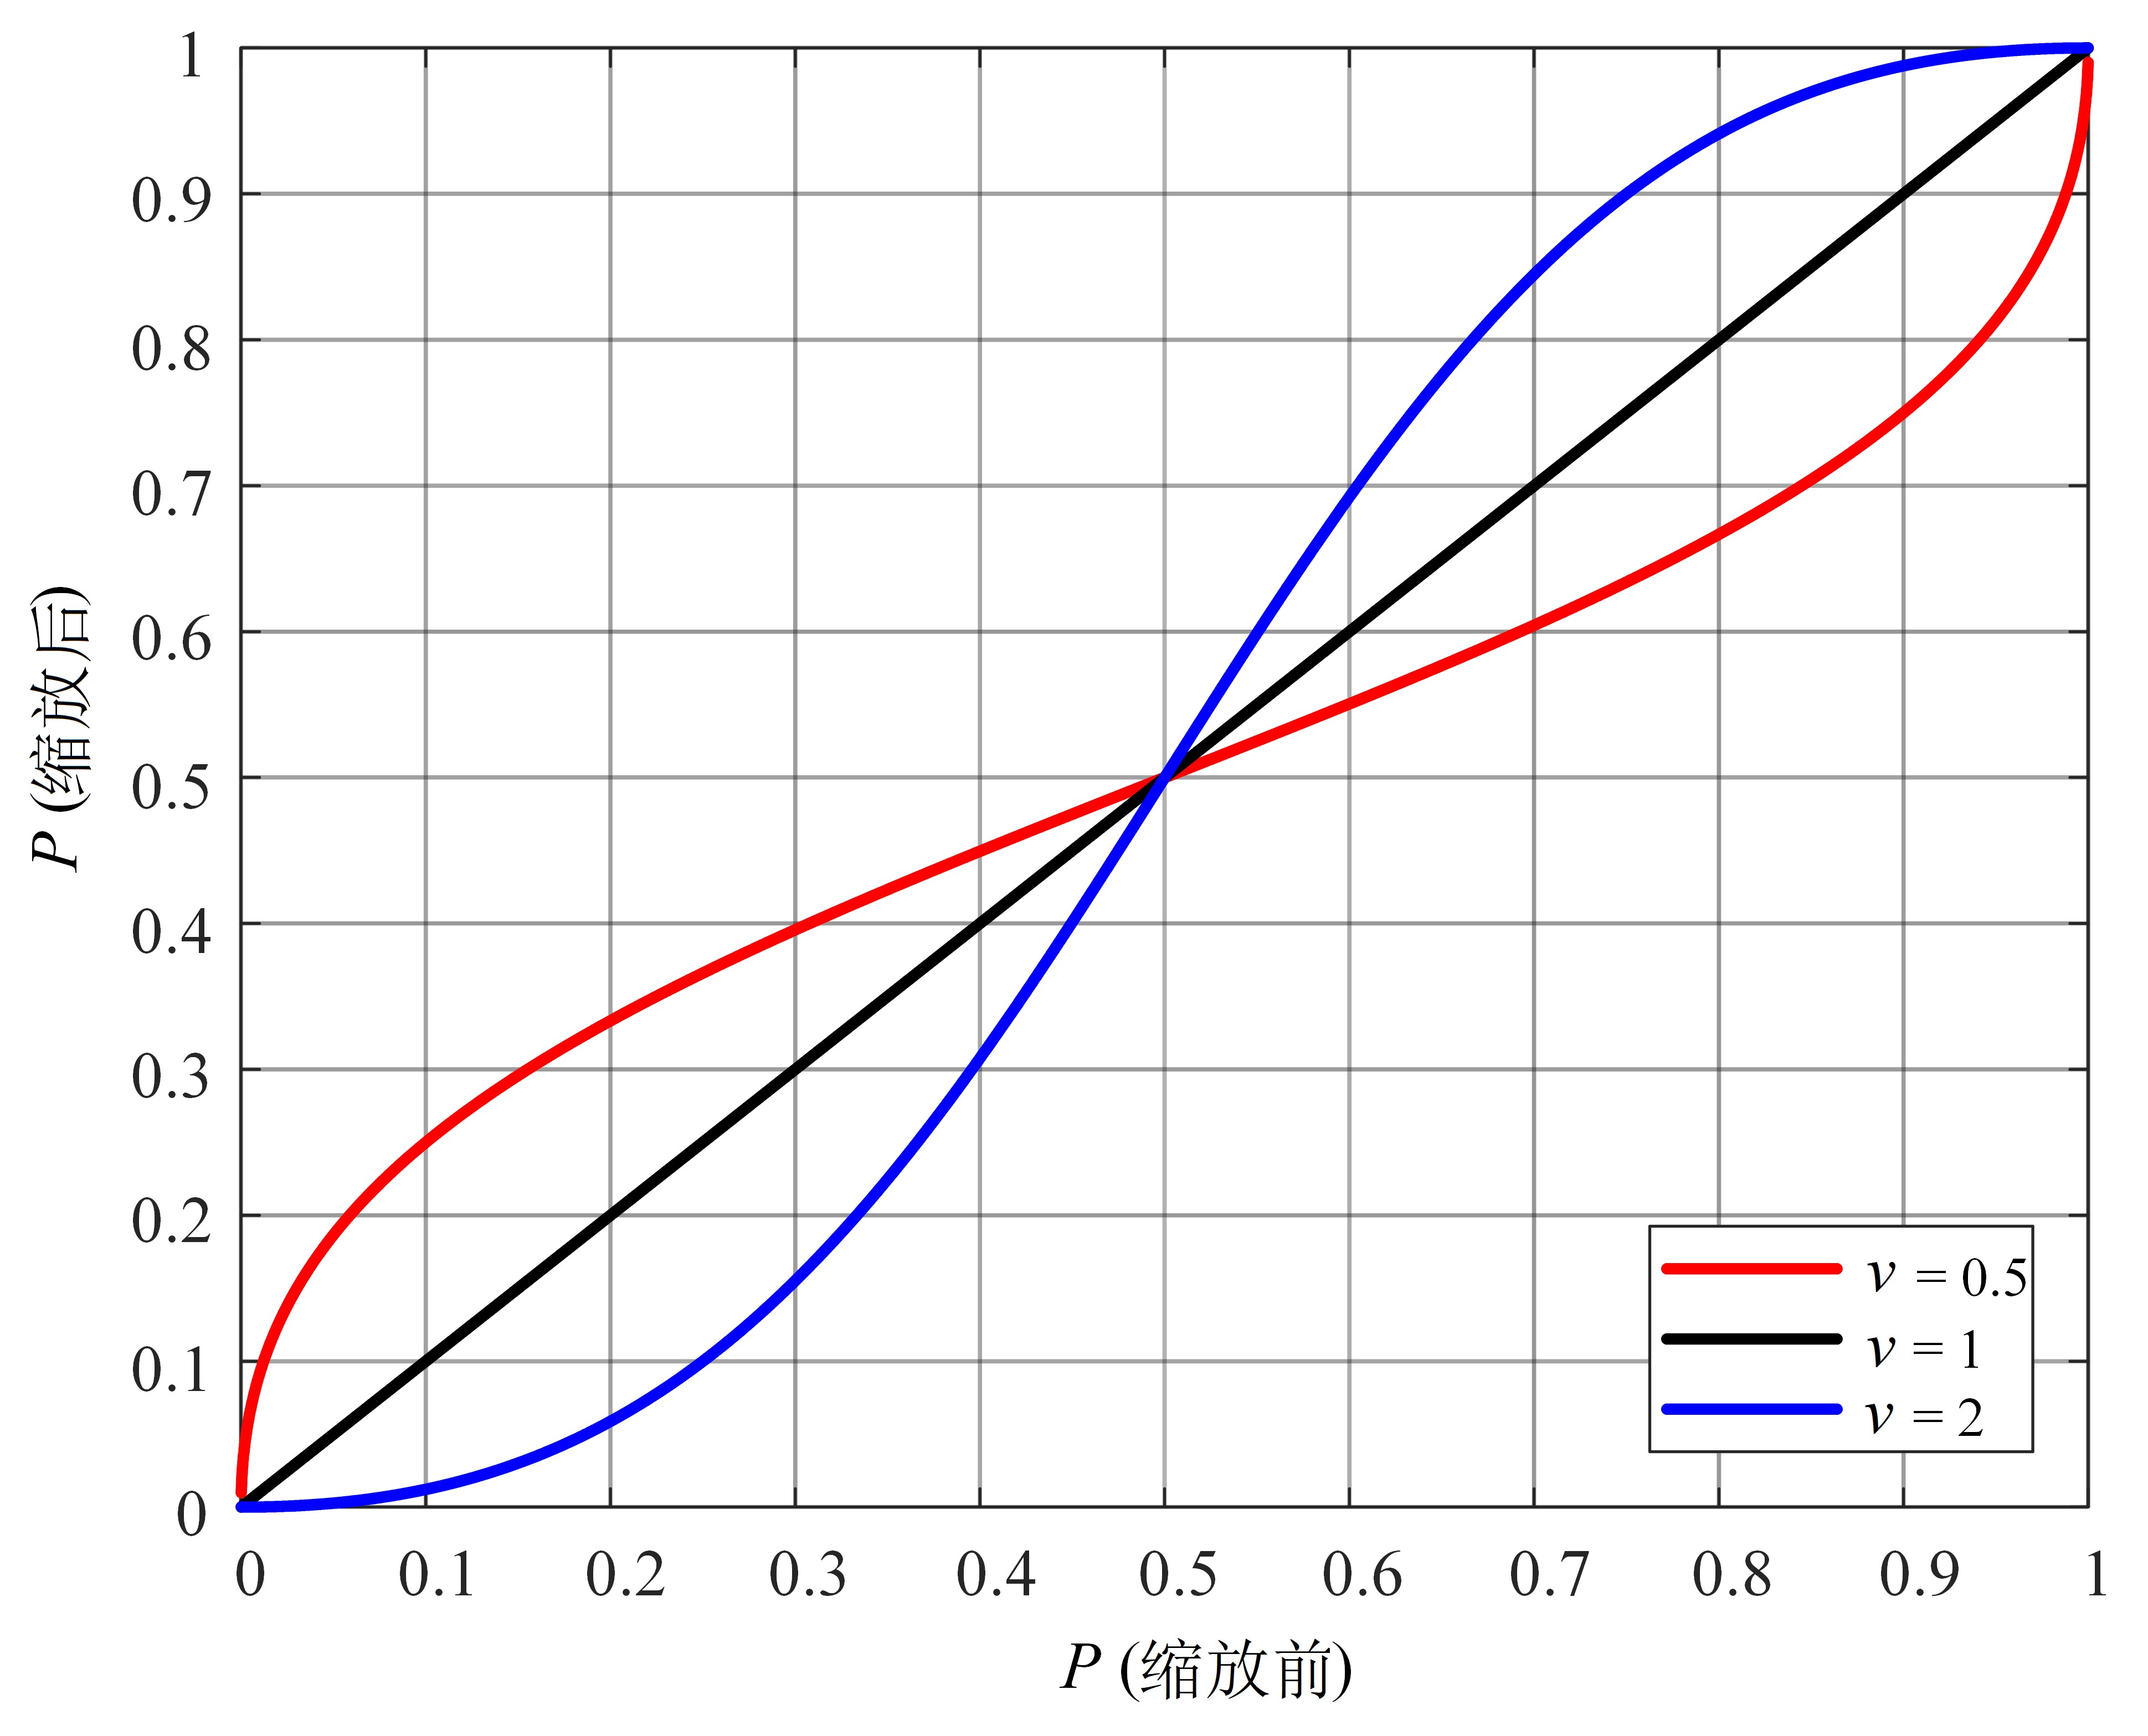
\includegraphics[width=10cm]{chapters/31}
	    \bicaption[\xiaosi 不同缩放系数v的缩放效果]{\wuhao 不同缩放系数v的缩放结果}{\wuhao Scaling results with different scaling coefficients ν}
	   	 \label{fig:3.1}
\end{figure}

%调整图片与下方文字之间的间距
\vspace{-0.35cm}

图片标题与图片之间的间距使用默认设置即可,与上下文的间距由于LATEX动态排版特性,需要大家手动调整。

。

。

。

。

。

。

。

。



下图是多子图示例:
%\vspace{-1cm}



\begin{figure}[h]
	\centering
	\subfigure[]{
		\label{fig:DE_J}
		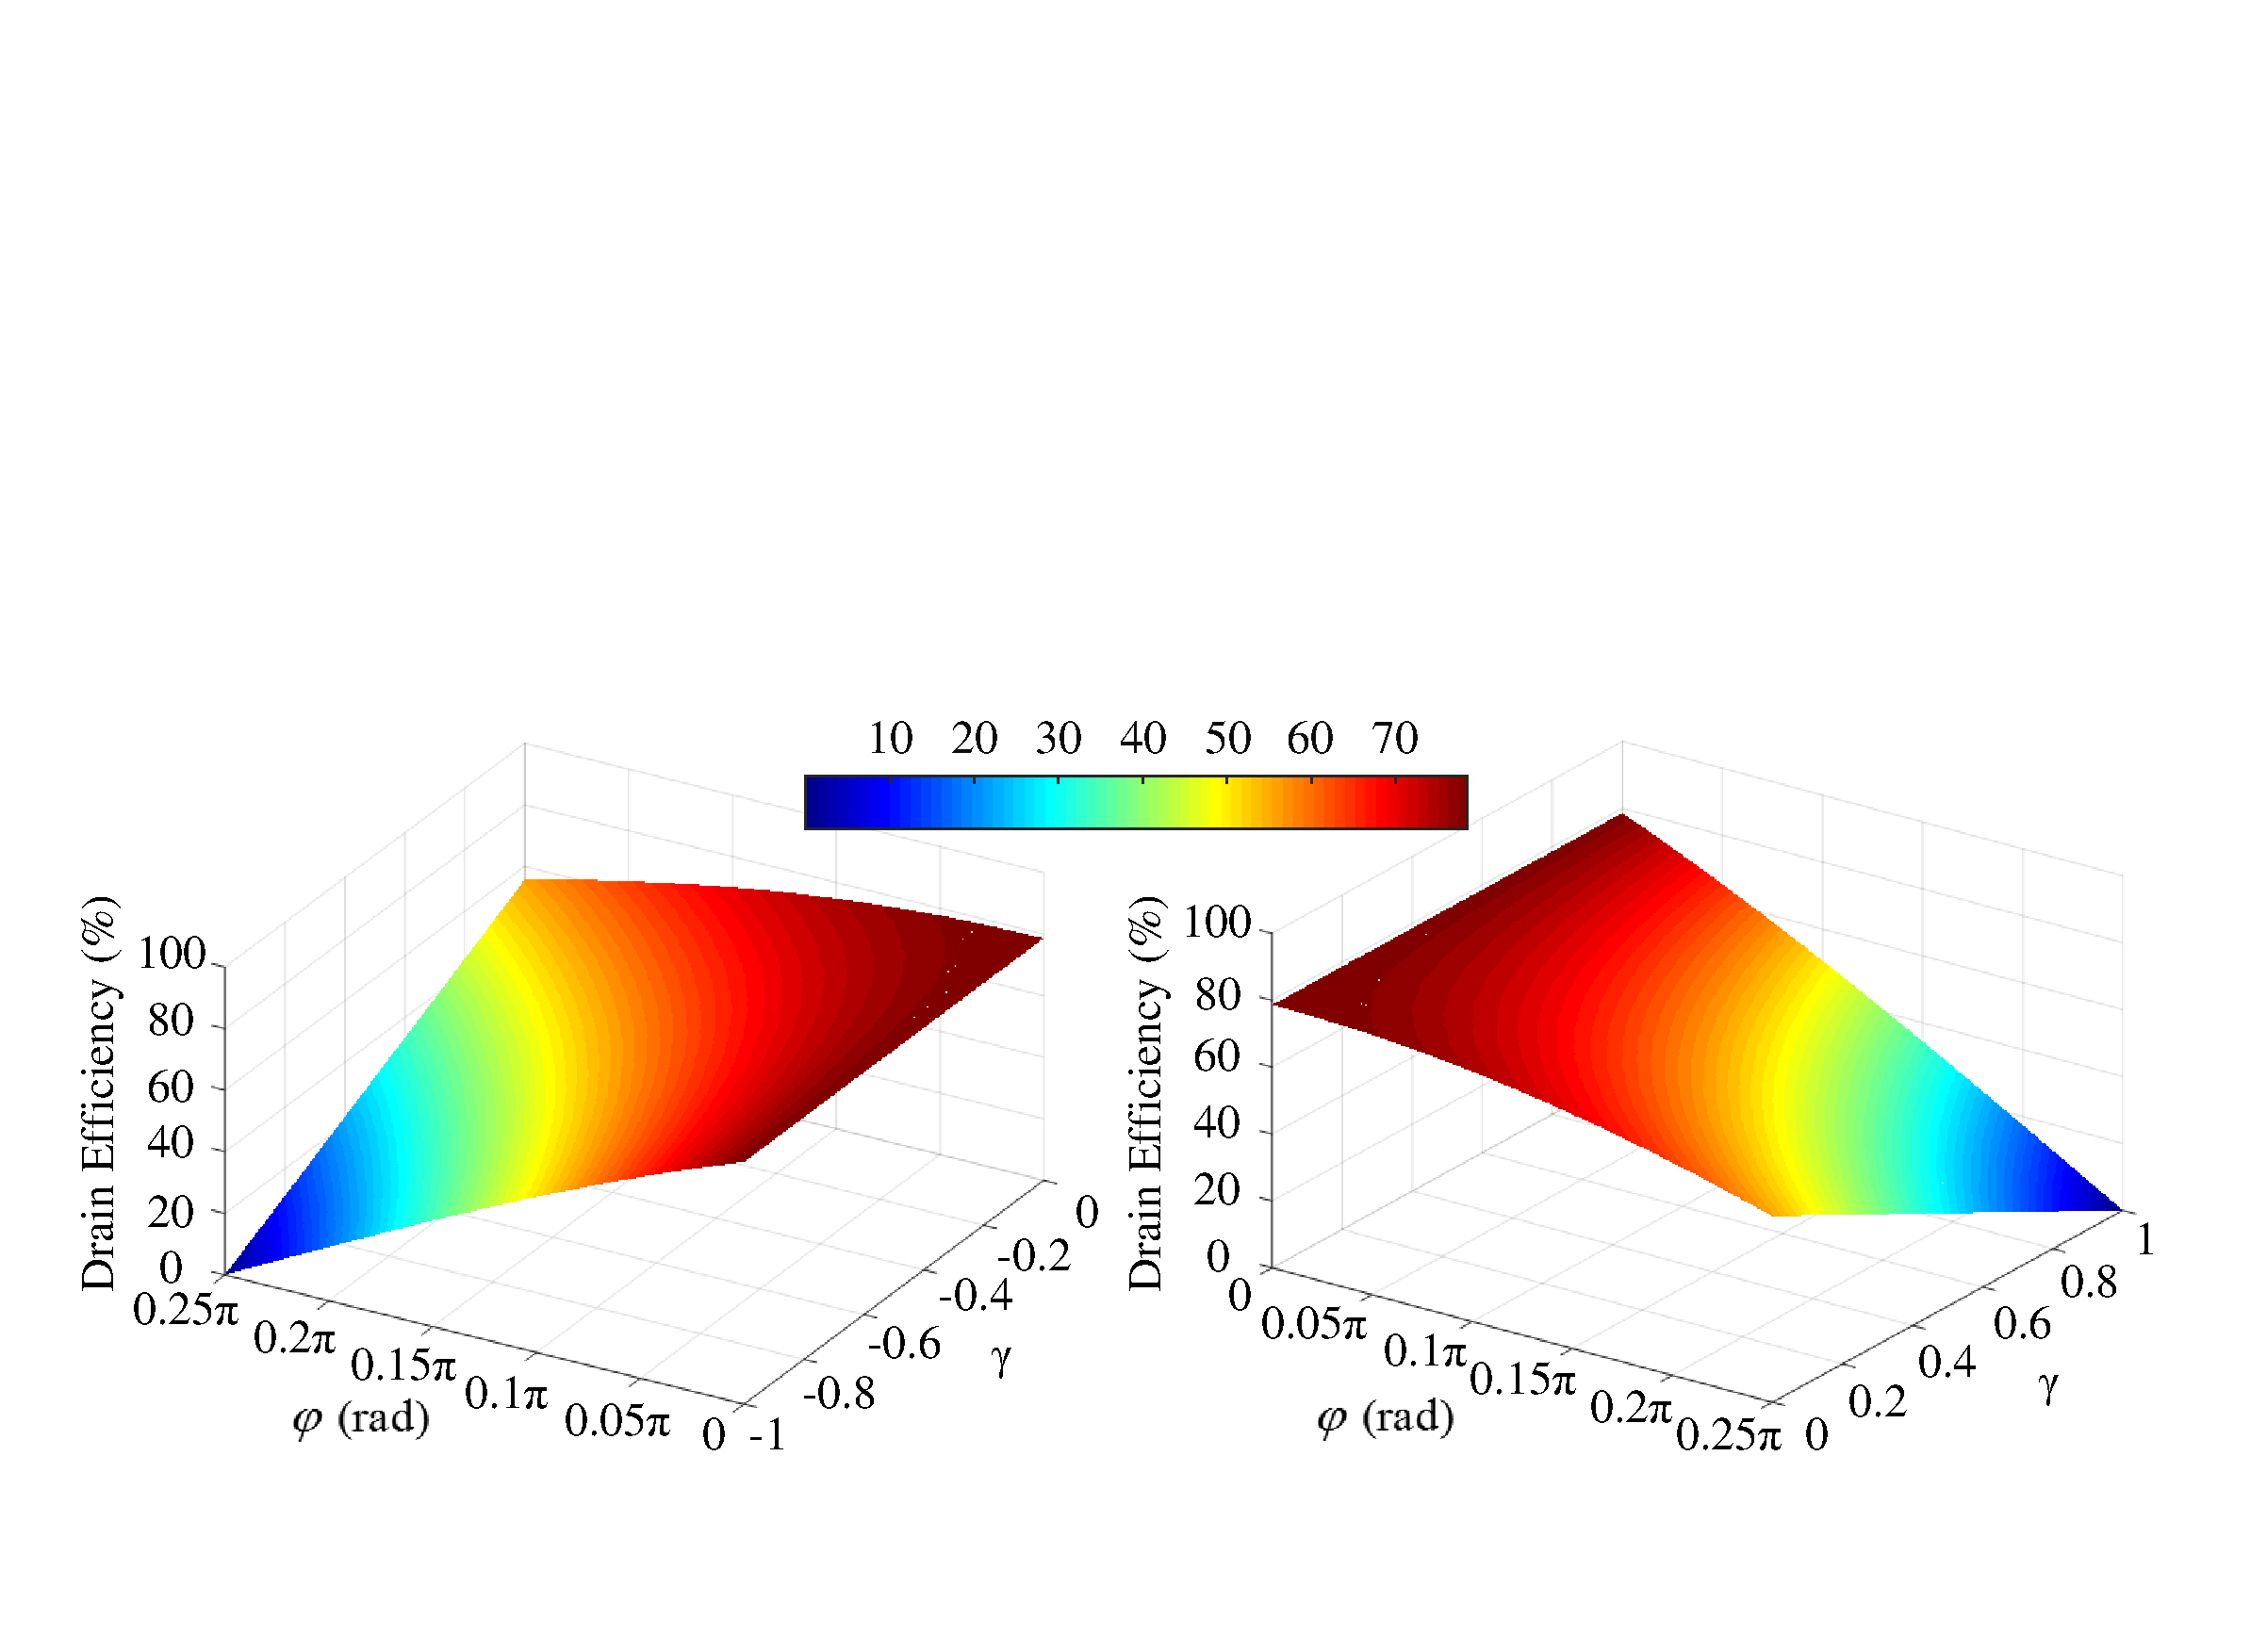
\includegraphics[width=12cm]{chapters/DE_J.pdf}}
	\subfigure[]{
		\label{fig:DE_CF}
		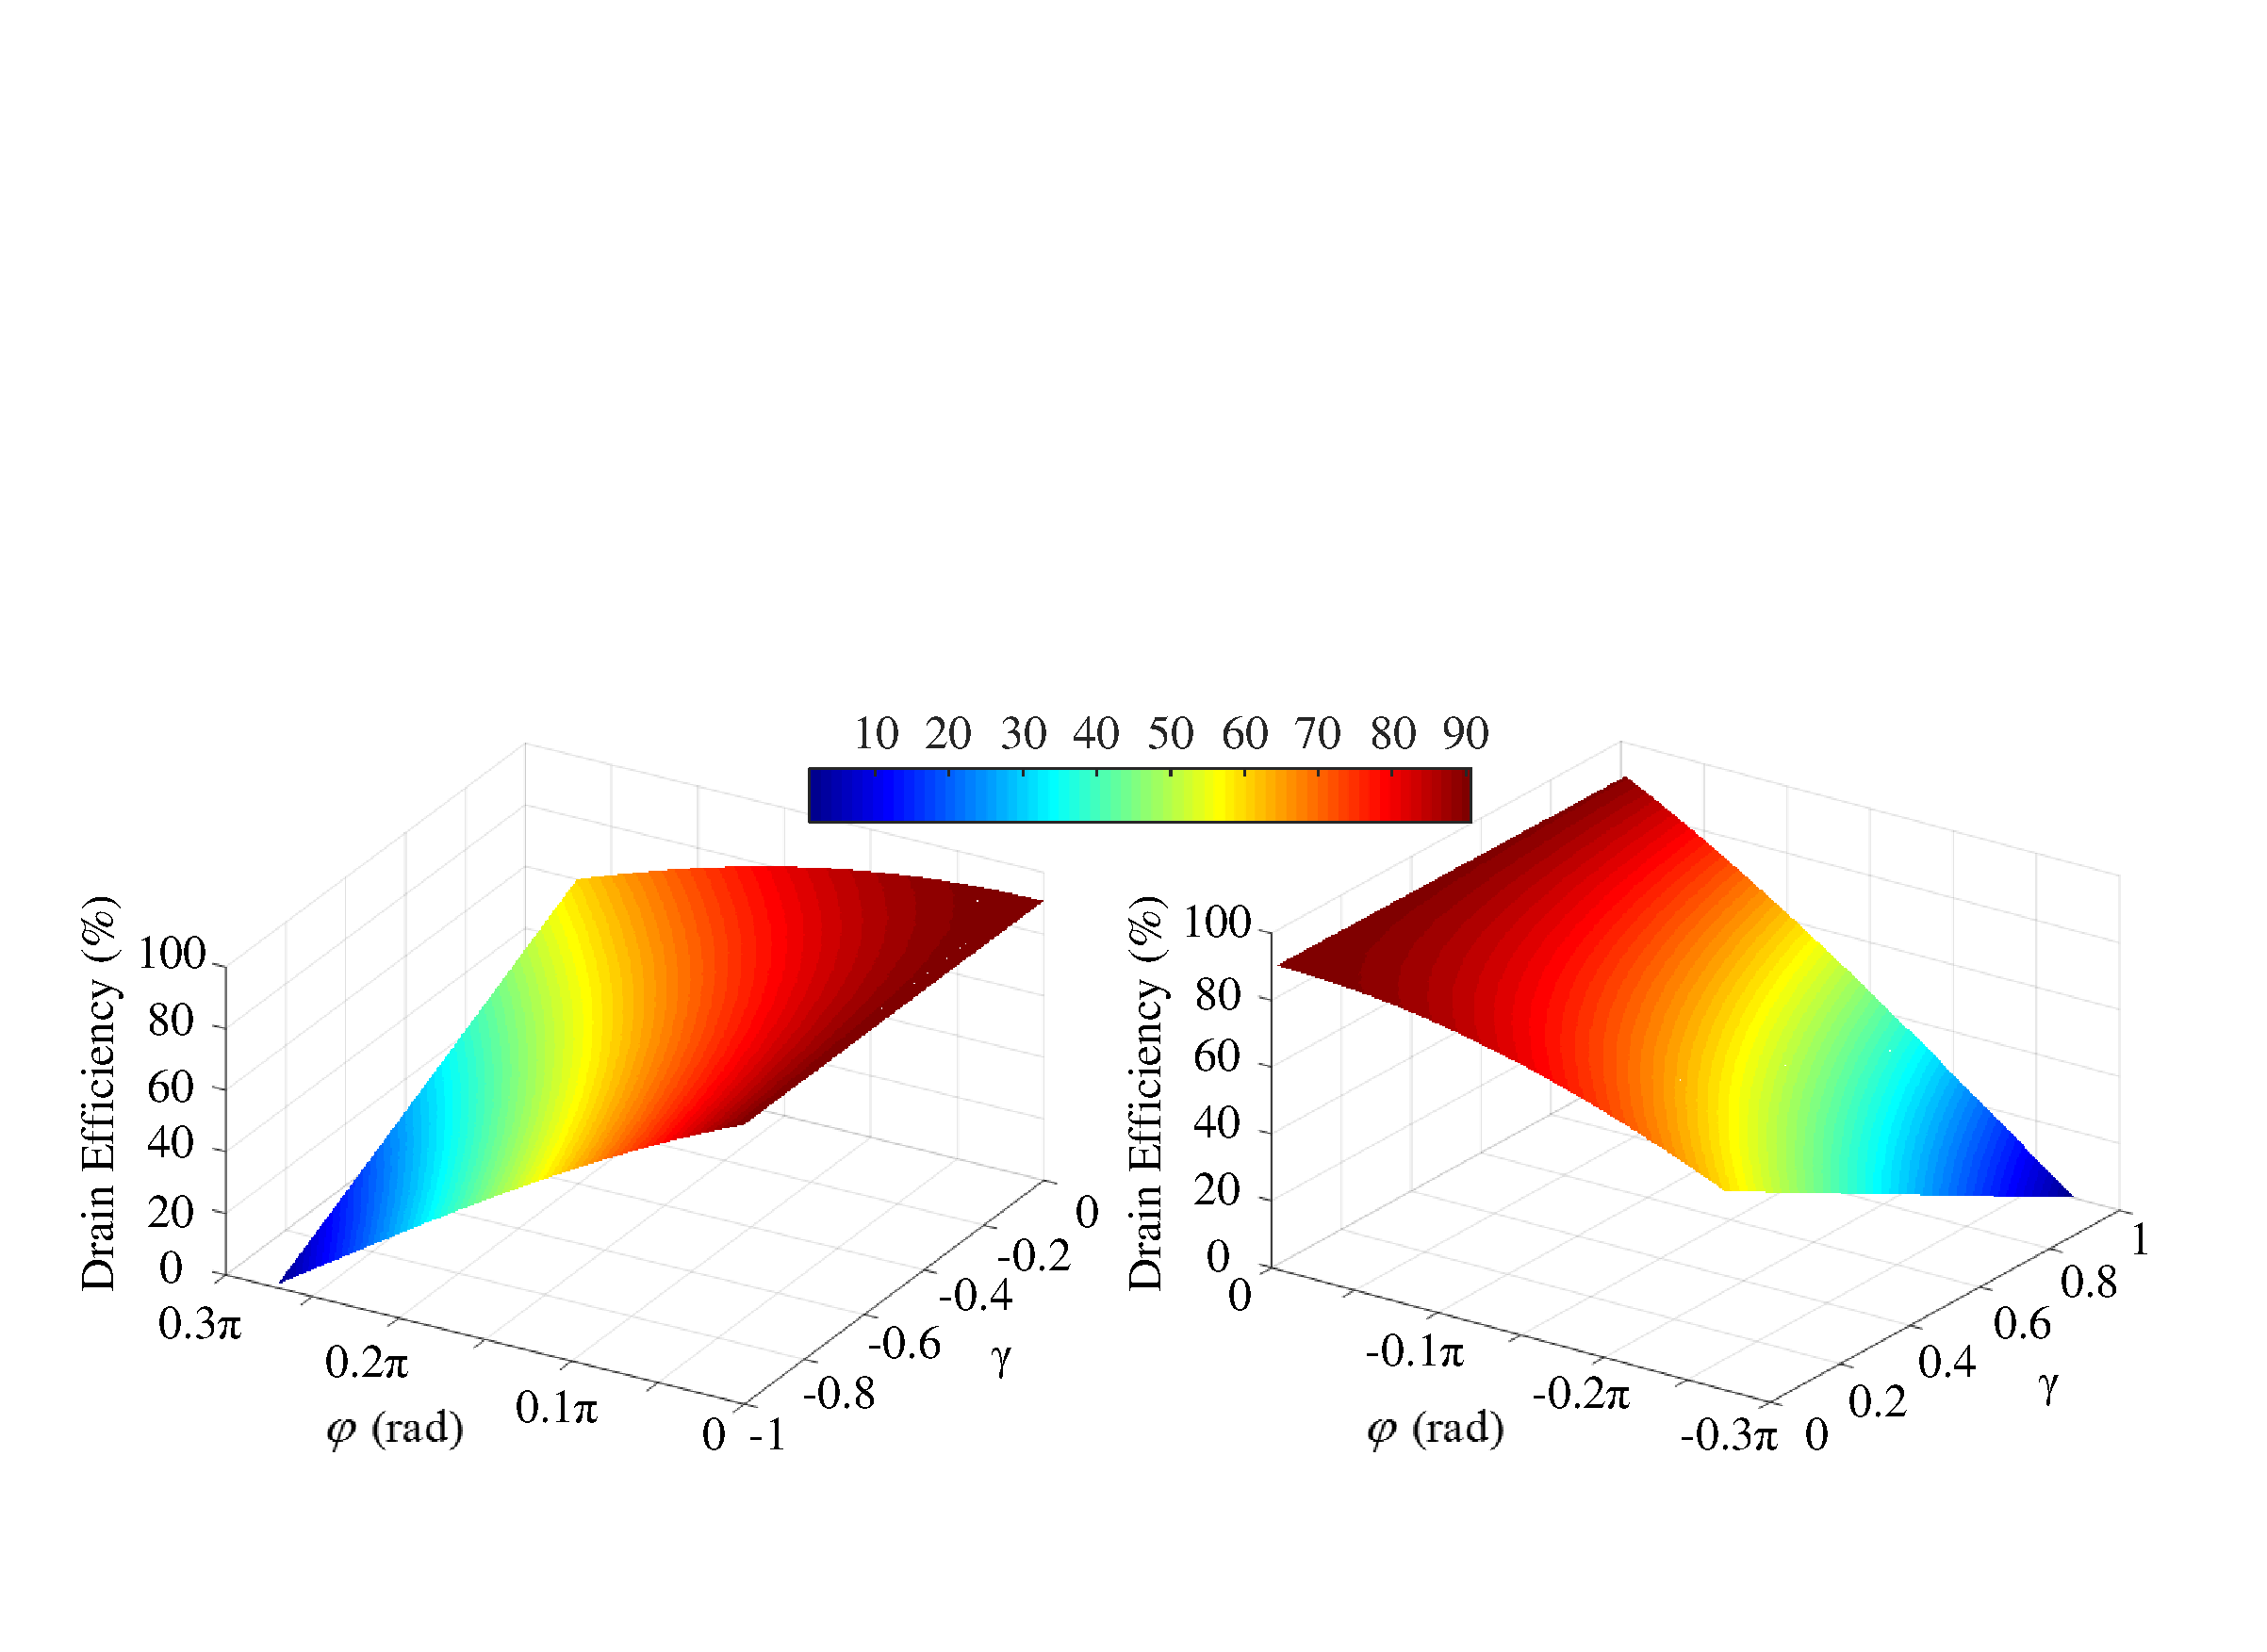
\includegraphics[width=12cm]{chapters/DE_CF.pdf}}   
\bicaption[\xiaosi 理论效率与$\gamma$和$\varphi$的关系。]{\wuhao 理论效率与$\gamma$和$\varphi$的关系。 (a) $\alpha=1$; (b) $\alpha=2/\sqrt{3}$}{\wuhao Theoretical DE versus $\gamma$ and $\varphi$. (a) $\alpha=1$; (b) $\alpha=2/\sqrt{3}$}

%	\caption{\wuhao 理论效率与$\gamma$和$\varphi$的关系。 (a) $\alpha=1$; (b) $\alpha=2/\sqrt{3}$}
%%	\raggedright
%	\wuhao Fig. 3-2 Theoretical DE versus $\gamma$ and $\varphi$. (a) $\alpha=1$. (b) $\alpha=2/\sqrt{3}$.Theoretical DE versus $\gamma$ and $\varphi$. (a) $\alpha=1$. (b) $\alpha=2/\sqrt{3}$.
\end{figure}

\vspace{-0.5cm}

\subsection{表}

表格格式参照写作指南。表格格式参照写作指南。表格格式参照写作指南。表格格式参照写作指南。表格格式参照写作指南。表格格式参照写作指南。表格格式参照写作指南。表格格式参照写作指南。表格格式参照写作指南。表格格式参照写作指南。表格格式参照写作指南。表格格式参照写作指南。表格格式参照写作指南。表格格式参照写作指南。表格格式参照写作指南。表格格式参照写作指南。

\vspace{0.1cm}

\begin{table}[h]
	\renewcommand{\arraystretch}{1.5}
	\centering
	\bicaption[\xiaosi 电流类型对效率的影响]{\wuhao 电流类型对效率的影响}{\wuhao Current type impact on efficiency}
	\begin{tabular}{p{3cm}p{3cm}p{3cm}p{3cm}}
		\toprule[1.5pt]
		\makecell[c]{\songti\wuhao 电流类型}&\makecell[c]{\songti\wuhao A}&\makecell[c]{\songti\wuhao B}&\makecell[c]{\songti\wuhao C}\\
		\hline
		\makecell[c]{\wuhao aaa}&\makecell[c]{\wuhao aa1}&\makecell[c]{\wuhao bb1}&\makecell[c]{\wuhao cc1}\\
		\bottomrule[1.5pt]
	\end{tabular}
   \label{tab:3.1} 	
\end{table}

表格格式参照写作指南。表格格式参照写作指南。表格格式参照写作指南。表格格式参照写作指南。表格格式参照写作指南。表格格式参照写作指南。表格格式参照写作指南。表格格式参照写作指南。表格格式参照写作指南。表格格式参照写作指南。表格格式参照写作指南。表格格式参照写作指南。表格格式参照写作指南。表格格式参照写作指南。表格格式参照写作指南。表格格式参照写作指南。

\vspace{-0.1cm}

\begin{table*}[h]
	\renewcommand{\arraystretch}{1.5}
	\bicaption[\xiaosi 高效率功放性能对比]{\wuhao 高效率功放性能对比}{\wuhao High-effiency power amplifier performance comparison}
	\label{tab_1}
	\centering
	\wuhao
	\begin{tabular}{c c c c c }
		\hline
		{\textbf{带宽}(GHz)}&{\textbf{功率}(dBm)}&{\textbf{效率}(\%)}&{\textbf{线性度}(dBc)}&{\textbf{信号带宽}(MHz)}\\
		\hline
		1.4--2.6&32--34&30--40 (DE)&-25 -- -30 (ACLR)&5\\
		\hline
		\multirow{2}{*}{2.1--2.7}&39&45 (DE) @ 2.14 GHz&--31 (ACLR)&\multirow{2}{*}{5}\\\cline{3-4}
		&(average)&40 (DE) @ 2.655 GHz&--30 (ACLR)&\\
		\hline
		3.5&38.1&59 (PAE)&30 (C/I)&5\\
		\hline
		\multirow{2}{*}{1.6--2.6}&36.0--38.5&45--60 (PAE)&30 (C/I)&5\\\cline{2-5}
		&35.3--37.5&40--55 (PAE)&--30 (ACLR)&20\\
		\hline
	\end{tabular}
\end{table*}


\section{公式格式}

\begin{equation}
\left\{ \begin{aligned}
0.794 \le \zeta  \le 1 ~~~~~~~~~~~\\
0.631 \le \gamma  = \frac{{0.631}}{{{\zeta ^2}}} \le 1~~~~~~ \\
- \frac{1}{{2\gamma }} \le \delta  \le \frac{1}{{2\gamma }}~~~~~~~~~~~ \\
{Z_{c,low,f}} = 2{R_{opt}}(\gamma  + j\delta )~~~~~\\
{Z_{c,2f}} = {Z_{c,low,2f}} =  - j\frac{{3\pi }}{4}\gamma \delta {R_{opt}}
\end{aligned} \right.
\label{eq:3.1}
\end{equation}

\begin{equation}
\begin{aligned}
v(\theta ) = V_{DD}\cdot(1 - \alpha cos(\theta  + \varphi ) + \beta cos(3\theta  + 3\varphi ))\\
\cdot(1 - \gamma \sin (\theta  + \varphi )) ~~~~~- 1 \le \gamma  \le 1\
\end{aligned}
\label{eq:vd}
\end{equation}




\noindent
公式格式测试。${\mathbf{\Theta }} = \left\{ {{\theta _k}\left( n \right),\forall k,n} \right\}$

\section{印制要求}
涉密学位论文的印刷、制作、传递、存档等,须符合国家、学校相关保密要求。学位论文一律左侧装订。

中文摘要之前的前置部分(封面、中、英文题名页、独创性声明和使用授权书),采用单面印刷。

从中文摘要开始,采用双面印刷。

中文摘要及之后的前置部分,包括中文摘要、ABSTRACT、目录、图目录(如有)、表目录(如有)、主要符号表(如有)、缩略词表(如有),在双面印刷时,若某部分页数为奇数,则该部分最后一页单面印刷。例如:若“摘要”只有1页,则其页码是“Ⅰ”,第“Ⅰ”页纸的背面为空白(无页眉或页码);“ABSTRACT”用新的一张纸印刷,页码从“Ⅱ”开始。

从第1章第1页开始,至论文最后1页,所有页面均双面印刷。例如:若第1章的最后1页为第17页,则第2章的第1页在第17页的背面印刷,页码为“18”(页眉是“重庆邮电大学博士(硕士)学位论文”)。

一次性双面打印整本学位论文技巧:除用于打印的版本外,电子版论文中一律不得出现空白页。论文打印建议使用PDF格式。为方便一次性双面打印,有时可在单面印刷的部分(如封面、中、英文题名页、独创性声明和使用授权书),或者双面打印只有1页的某部分内容(如摘要、ABSTRACT等)后插入1页空白页,该空白页不编排页眉页码;论文中出现的页码应前后连续,不得中断。


\section{本章小结}
本章介绍了……
\backmatter

%取消后续章节的页眉上的章节编号
\renewcommand{\chaptermark}[1]{\markboth{#1}{}}

%参考文献
% %参考文献
% \begin{thebibliography}{200}
% \wuhao %设置参考文献字体大小
% \linespread{1}\selectfont
% \setlength{\itemsep}{-1.4ex} %缩小条目间行距
% \thispagestyle{others}
% \pagestyle{others}

% \makeatletter
% \renewcommand\@biblabel[1]{[#1]\hfill} %序号左对齐
% \makeatother
% \setlength{\labelsep}{0cm}

%   \providecommand{\bibauthor}[1]{#1}
%   \providecommand{\bibeditor}[1]{#1}
%   \providecommand{\bibtranslator}[1]{#1}
%   \providecommand{\bibtitle}[1]{#1}
%   \providecommand{\bibbooktitle}[1]{#1}
%   \providecommand{\bibjournal}[1]{#1}
%   \providecommand{\bibmark}[1]{#1}
%   \providecommand{\bibcountry}[1]{#1}
%   \providecommand{\bibpatentid}[1]{#1}
%   \providecommand{\bibedition}[1]{#1}
%   \providecommand{\biborganization}[1]{#1}
%   \providecommand{\bibaddress}[1]{#1}
%   \providecommand{\bibpublisher}[1]{#1}
%   \providecommand{\bibinstitution}[1]{#1}
%   \providecommand{\bibschool}[1]{#1}
%   \providecommand{\bibvolume}[1]{#1}
%   \providecommand{\bibnumber}[1]{#1}
%   \providecommand{\bibpages}[1]{#1}
%   \providecommand{\bibmodifydate}[1]{#1}
%   \providecommand{\bibcitedate}[1]{#1}
%   \providecommand{\bibyear}[1]{#1}
%   \providecommand{\bibdate}[1]{#1}
%   \providecommand{\biburl}[1]{\url{#1}}
  
%   \bibitem{PointNetVLAD}
%   \bibauthor{UY M~A\@, LEE G~H}\@. \bibtitle{PointNetVLAD: Deep point cloud based
%     retrieval for large-scale place recognition}\bibmark{[C]}\@.
%     \bibbooktitle{IEEE/CVF Conference on Computer Vision and Pattern
%     Recognition}\@, \bibaddress{Salt Lake City, USA}\@,
%     \bibyear{2018}\thinspace{}\textnormal{:
%     }\bibpages{4470\thinspace{}\textnormal{--}\thinspace{}4479}\@.
  
%   \bibitem{文物}
%   \bibauthor{赵夫群\@, 周明全}\@.
%     \bibtitle{文物点云模型的优化配准算法}\bibmark{[J]}\@.
%     \bibjournal{计算机应用研究}\@, \bibyear{2017}\@,
%     \bibvolume{34}\bibnumber{(12)}\thinspace{}\textnormal{: }\bibpages{4}\@.
  
%   \bibitem{逆向工程}
%   \bibauthor{宋丽梅}\@.
%     \bibtitle{双目立体机器视觉检测系统及其应用}\bibmark{[J]}\@.
%     \bibjournal{西南科技大学学报}\@, \bibyear{2006}\@,
%     \bibvolume{21}\bibnumber{(1)}\thinspace{}\textnormal{:
%     }\bibpages{30\thinspace{}\textnormal{--}\thinspace{}34}\@.
  
%   \bibitem{Map-matching}
%   \bibauthor{SOBREIRA H\@, COSTA C~M\@, SOUSA I, et~al}\@. \bibtitle{Map-matching
%     algorithms for robot self-localization: a comparison between perfect match,
%     iterative closest point and normal distributions transform}\bibmark{[J]}\@.
%     \bibjournal{Intelligent \& Robotic Systems}\@, \bibyear{2019}\@,
%     \bibvolume{93}\thinspace{}\textnormal{:
%     }\bibpages{533\thinspace{}\textnormal{--}\thinspace{}546}\@.
  
%   \bibitem{LCDNet}
%   \bibauthor{CATTANEO D\@, VAGHI M\@, VALADA A}\@. \bibtitle{LCDNet: Deep loop
%     closure detection and point cloud registration for LiDAR
%     SLAM}\bibmark{[J]}\@. \bibjournal{IEEE Transactions on Robotics}\@,
%     \bibyear{2022}\@, \bibvolume{38}\bibnumber{(4)}\thinspace{}\textnormal{:
%     }\bibpages{2074\thinspace{}\textnormal{--}\thinspace{}2093}\@.
  
%   \bibitem{LPD}
%   \bibauthor{LIU Z\@, ZHOU S\@, SUO C, et~al}\@. \bibtitle{LPD-Net: 3D point
%     cloud learning for large-scale place recognition and environment
%     analysis}\bibmark{[C]}\@. \bibbooktitle{IEEE/CVF International Conference on
%     Computer Vision}\@, \bibaddress{Seoul, Korea}\@,
%     \bibyear{2019}\thinspace{}\textnormal{:
%     }\bibpages{2831\thinspace{}\textnormal{--}\thinspace{}2840}\@.
  
%   \bibitem{2015review}
%   \bibauthor{POMERLEAU F\@, COLAS F\@, SIEGWART R, et~al}\@. \bibtitle{A review
%     of point cloud registration algorithms for mobile robotics}\bibmark{[J]}\@.
%     \bibjournal{Foundations and Trends{\textregistered} in Robotics}\@,
%     \bibyear{2015}\@, \bibvolume{4}\bibnumber{(1)}\thinspace{}\textnormal{:
%     }\bibpages{1\thinspace{}\textnormal{--}\thinspace{}104}\@.
  
%   \bibitem{ICP}
%   \bibauthor{BESL P\@, MCKAY N~D}\@. \bibtitle{A method for registration of 3-D
%     shapes}\bibmark{[J]}\@. \bibjournal{IEEE Transactions on Pattern Analysis and
%     Machine Intelligence}\@, \bibyear{1992}\@,
%     \bibvolume{14}\bibnumber{(2)}\thinspace{}\textnormal{:
%     }\bibpages{239\thinspace{}\textnormal{--}\thinspace{}256}\@.
  
%   \bibitem{1998}
%   \bibauthor{GOLD S\@, RANGARAJAN A\@, LU C-P, et~al}\@. \bibtitle{New algorithms
%     for 2D and 3D point matching: pose estimation and
%     correspondence}\bibmark{[J]}\@. \bibjournal{Pattern Recognition}\@,
%     \bibyear{1998}\@, \bibvolume{31}\bibnumber{(8)}\thinspace{}\textnormal{:
%     }\bibpages{1019\thinspace{}\textnormal{--}\thinspace{}1031}\@.
  
%   \bibitem{Go-ICP}
%   \bibauthor{YANG J\@, LI H\@, JIA Y}\@. \bibtitle{Go-ICP: Solving 3D
%     registration efficiently and globally optimally}\bibmark{[C]}\@.
%     \bibbooktitle{IEEE/CVF International Conference on Computer Vision}\@,
%     \bibaddress{Sydney, Australia}\@, \bibyear{2013}\thinspace{}\textnormal{:
%     }\bibpages{1457\thinspace{}\textnormal{--}\thinspace{}1464}\@.
  
%   \bibitem{Almohamad}
%   \bibauthor{ALMOHAMAD H\@, DUFFUAA S~O}\@. \bibtitle{A linear programming
%     approach for the weighted graph matching problem}\bibmark{[J]}\@.
%     \bibjournal{IEEE Transactions on pattern analysis and machine
%     intelligence}\@, \bibyear{1993}\@,
%     \bibvolume{15}\bibnumber{(5)}\thinspace{}\textnormal{:
%     }\bibpages{522\thinspace{}\textnormal{--}\thinspace{}525}\@.
  
%   \bibitem{CSGM}
%   \bibauthor{HUANG X\@, ZHANG J\@, FAN L, et~al}\@. \bibtitle{A systematic
%     approach for cross-source point cloud registration by preserving macro and
%     micro structures}\bibmark{[J]}\@. \bibjournal{IEEE Transactions on Image
%     Processing}\@, \bibyear{2017}\@,
%     \bibvolume{26}\bibnumber{(7)}\thinspace{}\textnormal{:
%     }\bibpages{3261\thinspace{}\textnormal{--}\thinspace{}3276}\@.
  
%   \bibitem{FGM}
%   \bibauthor{ZHOU F\@, De~la TORRE F}\@. \bibtitle{Factorized graph
%     matching}\bibmark{[C]}\@. \bibbooktitle{IEEE/CVF Conference on Computer
%     Vision and Pattern Recognition}\@, \bibaddress{Providence, USA}\@,
%     \bibyear{2012}\thinspace{}\textnormal{:
%     }\bibpages{127\thinspace{}\textnormal{--}\thinspace{}134}\@.
  
%   \bibitem{Leordeanu}
%   \bibauthor{LEORDEANU M\@, HEBERT M}\@. \bibtitle{A spectral technique for
%     correspondence problems using pairwise constraints}\bibmark{[C]}\@.
%     \bibbooktitle{IEEE/CVF International Conference on Computer Vision}\@,
%     \bibaddress{Beijing, China}\@, \bibyear{2005}\thinspace{}\textnormal{:
%     }\bibpages{1482\thinspace{}\textnormal{--}\thinspace{}1489}\@.
  
%   \bibitem{JRMPC}
%   \bibauthor{EVANGELIDIS G~D\@, KOUNADES-BASTIAN D\@, HORAUD R, et~al}\@.
%     \bibtitle{A generative model for the joint registration of multiple point
%     sets}\bibmark{[C]}\@. \bibbooktitle{European Conference on Computer
%     Vision}\@, \bibaddress{Zurich, Switzerland}\@, \bibyear{2014}\@.
  
%   \bibitem{CPD}
%   \bibauthor{MYRONENKO A\@, SONG X}\@. \bibtitle{Point set registration: coherent
%     point drift}\bibmark{[J]}\@. \bibjournal{IEEE Transactions on Pattern
%     Analysis and Machine Intelligence}\@, \bibyear{2010}\@,
%     \bibvolume{32}\bibnumber{(12)}\thinspace{}\textnormal{:
%     }\bibpages{2262\thinspace{}\textnormal{--}\thinspace{}2275}\@.
  
%   \bibitem{CH-GMM}
%   \bibauthor{FAN J\@, YANG J\@, AI D, et~al}\@. \bibtitle{Convex hull indexed
%     Gaussian mixture model for 3D point set registration}\bibmark{[J]}\@.
%     \bibjournal{Pattern Recognition}\@, \bibyear{2016}\@,
%     \bibvolume{59}\thinspace{}\textnormal{:
%     }\bibpages{126\thinspace{}\textnormal{--}\thinspace{}141}\@.
  
%   \bibitem{PointNetLK}
%   \bibauthor{AOKI Y\@, GOFORTH H\@, SRIVATSAN R~A, et~al}\@.
%     \bibtitle{PointNetLK: robust \& efficient point cloud registration ssing
%     pointNet}\bibmark{[C]}\@. \bibbooktitle{IEEE/CVF Conference on Computer
%     Vision and Pattern Recognition}\@, \bibaddress{Seoul, Korea}\@,
%     \bibyear{2019}\thinspace{}\textnormal{:
%     }\bibpages{7156\thinspace{}\textnormal{--}\thinspace{}7165}\@.
  
%   \bibitem{LucasKanade}
%   \bibauthor{BAKER S\@, MATTHEWS I}\@. \bibtitle{Lucas-Kanade 20 years on: A
%     unifying framework}\bibmark{[J]}\@. \bibjournal{International Journal of
%     Computer Vision}\@, \bibyear{2004}\@, \bibvolume{56}\thinspace{}\textnormal{:
%     }\bibpages{221\thinspace{}\textnormal{--}\thinspace{}255}\@.
  
%   \bibitem{PPF}
%   \bibauthor{DENG H\@, BIRDAL T\@, ILIC S}\@. \bibtitle{PPFNet: Global context
%     aware local features for robust 3D point matching}\bibmark{[C]}\@.
%     \bibbooktitle{IEEE/CVF Conference on Computer Vision and Pattern
%     Recognition}\@, \bibaddress{Salt Lake City, USA}\@,
%     \bibyear{2018}\thinspace{}\textnormal{:
%     }\bibpages{195\thinspace{}\textnormal{--}\thinspace{}205}\@.
  
%   \bibitem{FMR}
%   \bibauthor{HUANG X\@, MEI G\@, ZHANG J}\@. \bibtitle{Feature-Metric
%     registration: A fast semi-Supervised approach for robust point cloud
%     registration without correspondences}\bibmark{[C]}\@. \bibbooktitle{IEEE/CVF
%     Conference on Computer Vision and Pattern Recognition}\@,
%     \bibaddress{Seattle, USA}\@, \bibyear{2020}\thinspace{}\textnormal{:
%     }\bibpages{11363\thinspace{}\textnormal{--}\thinspace{}11371}\@.
  
%   \bibitem{OMNet}
%   \bibauthor{XU H\@, LIU S\@, WANG G, et~al}\@. \bibtitle{OMNet: Learning
%     overlapping mask for partial-to-partial point cloud
%     registration}\bibmark{[C]}\@. \bibbooktitle{IEEE/CVF International Conference
%     on Computer Vision}\@, \bibaddress{Montreal, Canada}\@,
%     \bibyear{2021}\thinspace{}\textnormal{:
%     }\bibpages{3112\thinspace{}\textnormal{--}\thinspace{}3121}\@.
  
%   \bibitem{PointNet}
%   \bibauthor{CHARLES R~Q\@, SU H\@, KAICHUN M, et~al}\@. \bibtitle{PointNet: Deep
%     learning on point sets for 3D classification and
%     segmentation}\bibmark{[C]}\@. \bibbooktitle{IEEE/CVF Conference on Computer
%     Vision and Pattern Recognition}\@, \bibaddress{Honolulu, USA}\@,
%     \bibyear{2017}\thinspace{}\textnormal{:
%     }\bibpages{77\thinspace{}\textnormal{--}\thinspace{}85}\@.
  
%   \bibitem{PointNet++}
%   \bibauthor{QI R\@, YI L\@, SU H, et~al}\@. \bibtitle{Pointnet++: Deep
%     hierarchical feature learning on point sets in a metric
%     space}\bibmark{[J]}\@. \bibjournal{Advances in Neural Information Processing
%     Systems}\@, \bibyear{2017}\@, \bibvolume{30}\thinspace{}\textnormal{:
%     }\bibpages{5099\thinspace{}\textnormal{--}\thinspace{}5108}\@.
  
%   \bibitem{3DFeat-Net}
%   \bibauthor{YEW Z~J\@, LEE G~H}\@. \bibtitle{3DFeat-Net: Weakly supervised local
%     3D features for point cloud registration}\bibmark{[C]}\@.
%     \bibbooktitle{European Conference on Computer Vision}\@, \bibaddress{Munich,
%     Germany}\@, \bibyear{2018}\thinspace{}\textnormal{:
%     }\bibpages{630\thinspace{}\textnormal{--}\thinspace{}646}\@.
  
%   \bibitem{PerfectMatch}
%   \bibauthor{GOJCIC Z\@, ZHOU C\@, WEGNER J~D, et~al}\@. \bibtitle{The Perfect
%     Match: 3D Point Cloud Matching With Smoothed Densities}\bibmark{[C]}\@.
%     \bibbooktitle{IEEE/CVF Conference on Computer Vision and Pattern
%     Recognition}\@, \bibaddress{Long Beach, USA}\@,
%     \bibyear{2019}\thinspace{}\textnormal{:
%     }\bibpages{5540\thinspace{}\textnormal{--}\thinspace{}5549}\@.
  
%   \bibitem{DGCNN}
%   \bibauthor{WANG Y\@, SUN Y\@, LIU Z, et~al}\@. \bibtitle{Dynamic graph cnn for
%     learning on point clouds}\bibmark{[J]}\@. \bibjournal{Acm Transactions On
%     Graphics}\@, \bibyear{2019}\@,
%     \bibvolume{38}\bibnumber{(5)}\thinspace{}\textnormal{:
%     }\bibpages{1\thinspace{}\textnormal{--}\thinspace{}12}\@.
  
%   \bibitem{KPConv}
%   \bibauthor{THOMAS H\@, QI C~R\@, DESCHAUD J-E, et~al}\@. \bibtitle{KPConv:
%     Flexible and deformable convolution for point clouds}\bibmark{[C]}\@.
%     \bibbooktitle{IEEE/CVF International Conference on Computer Vision}\@,
%     \bibaddress{Seoul, Korea}\@, \bibyear{2019}\thinspace{}\textnormal{:
%     }\bibpages{6410\thinspace{}\textnormal{--}\thinspace{}6419}\@.
  
%   \bibitem{3DMatch}
%   \bibauthor{ZENG A\@, SONG S\@, NIEßNER M, et~al}\@. \bibtitle{3DMatch:
%     Learning local geometric descriptors from RGB-D
%     reconstructions}\bibmark{[C]}\@. \bibbooktitle{IEEE/CVF Conference on
%     Computer Vision and Pattern Recognition}\@, \bibaddress{Honolulu, USA}\@,
%     \bibyear{2017}\thinspace{}\textnormal{:
%     }\bibpages{199\thinspace{}\textnormal{--}\thinspace{}208}\@.
  
%   \bibitem{FCGF}
%   \bibauthor{CHOY C\@, PARK J\@, KOLTUN V}\@. \bibtitle{Fully convolutional
%     geometric features}\bibmark{[C]}\@. \bibbooktitle{IEEE/CVF International
%     Conference on Computer Vision}\@, \bibaddress{Seoul, Korea}\@,
%     \bibyear{2019}\thinspace{}\textnormal{:
%     }\bibpages{8957\thinspace{}\textnormal{--}\thinspace{}8965}\@.
  
%   \bibitem{SpinNet}
%   \bibauthor{AO S\@, HU Q\@, YANG B, et~al}\@. \bibtitle{Spinnet: Learning a
%     general surface descriptor for 3d point cloud registration}\bibmark{[C]}\@.
%     \bibbooktitle{IEEE/CVF Conference on Computer Vision and Pattern
%     Recognition}\@, \bibaddress{virtual}\@,
%     \bibyear{2021}\thinspace{}\textnormal{:
%     }\bibpages{11753\thinspace{}\textnormal{--}\thinspace{}11762}\@.
  
%   \bibitem{D3Feat}
%   \bibauthor{BAI X\@, LUO Z\@, ZHOU L, et~al}\@. \bibtitle{D3Feat: Joint learning
%     of dense detection and description of 3D local features}\bibmark{[C]}\@.
%     \bibbooktitle{IEEE/CVF Conference on Computer Vision and Pattern
%     Recognition}\@, \bibaddress{Seattle, USA}\@,
%     \bibyear{2020}\thinspace{}\textnormal{:
%     }\bibpages{6358\thinspace{}\textnormal{--}\thinspace{}6366}\@.
  
%   \bibitem{PREDATOR}
%   \bibauthor{HUANG S\@, GOJCIC Z\@, USVYATSOV M, et~al}\@. \bibtitle{PREDATOR:
%     Registration of 3D point clouds with low overlap}\bibmark{[C]}\@.
%     \bibbooktitle{IEEE/CVF Conference on Computer Vision and Pattern
%     Recognition}\@, \bibaddress{virtual}\@,
%     \bibyear{2021}\thinspace{}\textnormal{:
%     }\bibpages{4265\thinspace{}\textnormal{--}\thinspace{}4274}\@.
  
%   \bibitem{PointDSC}
%   \bibauthor{BAI X\@, LUO Z\@, ZHOU L, et~al}\@. \bibtitle{PointDSC: Robust point
%     cloud registration using deep spatial consistency}\bibmark{[C]}\@.
%     \bibbooktitle{IEEE/CVF Conference on Computer Vision and Pattern
%     Recognition}\@, \bibaddress{virtual}\@,
%     \bibyear{2021}\thinspace{}\textnormal{:
%     }\bibpages{15854\thinspace{}\textnormal{--}\thinspace{}15864}\@.
  
%   \bibitem{DCP}
%   \bibauthor{WANG Y\@, SOLOMON J}\@. \bibtitle{Deep Closest Point: Learning
%     representations for point cloud registration}\bibmark{[C]}\@.
%     \bibbooktitle{IEEE/CVF International Conference on Computer Vision}\@,
%     \bibaddress{Seoul, Korea}\@, \bibyear{2019}\thinspace{}\textnormal{:
%     }\bibpages{3522\thinspace{}\textnormal{--}\thinspace{}3531}\@.
  
%   \bibitem{IDAM}
%   \bibauthor{LI J\@, ZHANG C\@, XU Z, et~al}\@. \bibtitle{Iterative
%     distance-aware similarity matrix convolution with mutual-supervised point
%     elimination for efficient point cloud registration}\bibmark{[C]}\@.
%     \bibbooktitle{European Conference on Computer Vision}\@, \bibaddress{Glasgow,
%     UK}\@, \bibyear{2020}\thinspace{}\textnormal{:
%     }\bibpages{378\thinspace{}\textnormal{--}\thinspace{}394}\@.
  
%   \bibitem{DGR}
%   \bibauthor{CHOY C\@, DONG W\@, KOLTUN V}\@. \bibtitle{Deep global
%     registration}\bibmark{[C]}\@. \bibbooktitle{IEEE/CVF Conference on Computer
%     Vision and Pattern Recognition}\@, \bibaddress{Seattle, USA}\@,
%     \bibyear{2020}\thinspace{}\textnormal{:
%     }\bibpages{2511\thinspace{}\textnormal{--}\thinspace{}2520}\@.
  
%   \bibitem{Dope}
%   \bibauthor{MIN T\@, SONG C\@, KIM E, et~al}\@. \bibtitle{Distinctiveness
%     oriented positional equilibrium for point cloud registration}\bibmark{[C]}\@.
%     \bibbooktitle{IEEE/CVF International Conference on Computer Vision}\@,
%     \bibaddress{Montreal, Canada}\@, \bibyear{2021}\thinspace{}\textnormal{:
%     }\bibpages{5490\thinspace{}\textnormal{--}\thinspace{}5498}\@.
  
%   \bibitem{Deeper}
%   \bibauthor{LI Q\@, HAN Z\@, WU X-M}\@. \bibtitle{Deeper Insights into Graph
%     Convolutional Networks for Semi-Supervised Learning}\bibmark{[C]}\@.
%     \bibbooktitle{Proceedings of the AAAI Conference on Artificial
%     Intelligence}\@, \bibaddress{New Orleans, USA}\@,
%     \bibyear{2018}\thinspace{}\textnormal{:
%     }\bibpages{3538\thinspace{}\textnormal{--}\thinspace{}3545}\@.
  
%   \bibitem{Measuring}
%   \bibauthor{CHEN D\@, LIN Y\@, LI W, et~al}\@. \bibtitle{Measuring and relieving
%     the over-smoothing problem for graph neural networks from the topological
%     view}\bibmark{[J]}\@. \bibjournal{Proceedings of the AAAI Conference on
%     Artificial Intelligence}\@, \bibyear{2020}\@,
%     \bibvolume{34}\bibnumber{(04)}\thinspace{}\textnormal{:
%     }\bibpages{3438\thinspace{}\textnormal{--}\thinspace{}3445}\@.
  
%   \bibitem{RANSAC}
%   \bibauthor{FISCHLER M~A\@, BOLLES R~C}\@. \bibtitle{Random sample consensus: a
%     paradigm for model fitting with applications to image analysis and automated
%     cartography}\bibmark{[J]}\@. \bibjournal{Communications of the ACM}\@,
%     \bibyear{1981}\@, \bibvolume{24}\bibnumber{(6)}\thinspace{}\textnormal{:
%     }\bibpages{381\thinspace{}\textnormal{--}\thinspace{}395}\@.
  
%   \bibitem{Temporal}
%   \bibauthor{YUAN Z\@, SONG X\@, BAI L, et~al}\@. \bibtitle{Temporal-channel
%     transformer for 3d lidar-based video object detection for autonomous
%     driving}\bibmark{[J]}\@. \bibjournal{IEEE Transactions on Circuits and
%     Systems for Video Technology}\@, \bibyear{2021}\@,
%     \bibvolume{32}\bibnumber{(4)}\thinspace{}\textnormal{:
%     }\bibpages{2068\thinspace{}\textnormal{--}\thinspace{}2078}\@.
  
%   \bibitem{L3Net}
%   \bibauthor{LU W\@, ZHOU Y\@, WAN G, et~al}\@. \bibtitle{L3-Net: Towards
%     learning based LiDAR localization for autonomous driving}\bibmark{[C]}\@.
%     \bibbooktitle{IEEE/CVF Conference on Computer Vision and Pattern
%     Recognition}\@, \bibaddress{Long Beach, USA}\@,
%     \bibyear{2019}\thinspace{}\textnormal{:
%     }\bibpages{6382\thinspace{}\textnormal{--}\thinspace{}6391}\@.
  
%   \bibitem{IMLSSLAM}
%   \bibauthor{DESCHAUD J-E}\@. \bibtitle{IMLS-SLAM: Scan-to-Model matching based
%     on 3D data}\bibmark{[C]}\@. \bibbooktitle{IEEE International Conference on
%     Robotics and Automation}\@, \bibaddress{Brisbane, Australia}\@,
%     \bibyear{2018}\thinspace{}\textnormal{:
%     }\bibpages{2480\thinspace{}\textnormal{--}\thinspace{}2485}\@.
  
%   \bibitem{Positioning}
%   \bibauthor{BENEDEK C\@, MAJDIK A\@, NAGY B, et~al}\@. \bibtitle{Positioning and
%     perception in LiDAR point clouds}\bibmark{[J]}\@. \bibjournal{Digital Signal
%     Processing}\@, \bibyear{2021}\@, \bibvolume{119}\thinspace{}\textnormal{:
%     }\bibpages{103193}\@.
  
%   \bibitem{Generative_Adversarial}
%   \bibauthor{TAN L\@, LIN X\@, NIU D, et~al}\@. \bibtitle{Projected generative
%     adversarial network for point cloud completion}\bibmark{[J]}\@.
%     \bibjournal{IEEE Transactions on Circuits and Systems for Video
%     Technology}\@, \bibyear{2023}\@,
%     \bibvolume{33}\bibnumber{(2)}\thinspace{}\textnormal{:
%     }\bibpages{771\thinspace{}\textnormal{--}\thinspace{}781}\@.
  
%   \bibitem{Single_Image}
%   \bibauthor{NGUYEN A-D\@, CHOI S\@, KIM W, et~al}\@. \bibtitle{Single-Image 3D
%     reconstruction: rethinking point cloud deformation}\bibmark{[J]}\@.
%     \bibjournal{IEEE Transactions on Neural Networks and Learning Systems}\@,
%     \bibyear{2022}\thinspace{}\textnormal{:
%     }\bibpages{1\thinspace{}\textnormal{--}\thinspace{}15}\@.
  
%   \bibitem{LPOT}
%   \bibauthor{WANG G}\@. \bibtitle{LPOT: Locality-Preserving gromov-wasserstein
%     discrepancy for nonrigid point set registration}\bibmark{[J]}\@.
%     \bibjournal{IEEE Transactions on Neural Networks and Learning Systems}\@,
%     \bibyear{2022}\thinspace{}\textnormal{:
%     }\bibpages{1\thinspace{}\textnormal{--}\thinspace{}13}\@.
  
%   \bibitem{Birds_Stone}
%   \bibauthor{GU C\@, CONG Y\@, SUN G}\@. \bibtitle{Three Birds, One Stone:
%     Unified laser-based 3D reconstruction across different media}\bibmark{[J]}\@.
%     \bibjournal{IEEE Transactions on Instrumentation and Measurement}\@,
%     \bibyear{2021}\@, \bibvolume{70}\thinspace{}\textnormal{:
%     }\bibpages{1\thinspace{}\textnormal{--}\thinspace{}12}\@.
  
%   \bibitem{INENet}
%   \bibauthor{WU Y\@, ZHANG Y\@, FAN X, et~al}\@. \bibtitle{INENet: Inliers
%     estimation network with similarity learning for partial overlapping
%     registration}\bibmark{[J]}\@. \bibjournal{IEEE Transactions on Circuits and
%     Systems for Video Technology}\@, \bibyear{2023}\@,
%     \bibvolume{33}\bibnumber{(3)}\thinspace{}\textnormal{:
%     }\bibpages{1413\thinspace{}\textnormal{--}\thinspace{}1426}\@.
  
%   \bibitem{Task_specific}
%   \bibauthor{ZHANG Z\@, DAI Y\@, FAN B, et~al}\@. \bibtitle{Learning a
%     task-specific descriptor for robust matching of 3D point
%     clouds}\bibmark{[J]}\@. \bibjournal{IEEE Transactions on Circuits and Systems
%     for Video Technology}\@, \bibyear{2022}\@,
%     \bibvolume{32}\bibnumber{(12)}\thinspace{}\textnormal{:
%     }\bibpages{8462\thinspace{}\textnormal{--}\thinspace{}8475}\@.
  
%   \bibitem{RANSAC_Hypotheses}
%   \bibauthor{YANG J\@, HUANG Z\@, QUAN S, et~al}\@. \bibtitle{Toward efficient
%     and robust metrics for RANSAC hypotheses and 3D rigid
%     registration}\bibmark{[J]}\@. \bibjournal{IEEE Transactions on Circuits and
%     Systems for Video Technology}\@, \bibyear{2022}\@,
%     \bibvolume{32}\bibnumber{(2)}\thinspace{}\textnormal{:
%     }\bibpages{893\thinspace{}\textnormal{--}\thinspace{}906}\@.
  
%   \bibitem{Graphite}
%   \bibauthor{SALEH M\@, DEHGHANI S\@, BUSAM B, et~al}\@. \bibtitle{Graphite:
%     Graph-Induced feature extraction for point cloud
%     registration}\bibmark{[C]}\@. \bibbooktitle{International Conference on 3D
%     Vision}\@, \bibaddress{virtual}\@, \bibyear{2020}\thinspace{}\textnormal{:
%     }\bibpages{241\thinspace{}\textnormal{--}\thinspace{}251}\@.
  
%   \bibitem{CoFiNet}
%   \bibauthor{YU H\@, LI F\@, SALEH M, et~al}\@. \bibtitle{Cofinet: Reliable
%     coarse-to-fine correspondences for robust pointcloud
%     registration}\bibmark{[J]}\@. \bibjournal{Advances in Neural Information
%     Processing Systems}\@, \bibyear{2021}\@,
%     \bibvolume{34}\thinspace{}\textnormal{:
%     }\bibpages{23872\thinspace{}\textnormal{--}\thinspace{}23884}\@.
  
%   \bibitem{Geometric}
%   \bibauthor{QIN Z\@, YU H\@, WANG C, et~al}\@. \bibtitle{Geometric transformer
%     for fast and robust point cloud registration}\bibmark{[C]}\@.
%     \bibbooktitle{IEEE/CVF Conference on Computer Vision and Pattern
%     Recognition}\@, \bibaddress{New Orleans, USA}\@,
%     \bibyear{2022}\thinspace{}\textnormal{:
%     }\bibpages{11133\thinspace{}\textnormal{--}\thinspace{}11142}\@.
  
%   \bibitem{Attention}
%   \bibauthor{VASWANI A\@, SHAZEER N\@, PARMAR N, et~al}\@. \bibtitle{Attention is
%     all you need}\bibmark{[J]}\@. \bibjournal{Advances in Neural Information
%     Processing Systems}\@, \bibyear{2017}\@,
%     \bibvolume{30}\thinspace{}\textnormal{:
%     }\bibpages{5998\thinspace{}\textnormal{--}\thinspace{}6008}\@.
  
%   \bibitem{NMS}
%   \bibauthor{LOWE D~G}\@. \bibtitle{Distinctive image features from
%     scale-invariant keypoints}\bibmark{[J]}\@. \bibjournal{International Journal
%     of Computer Vision}\@, \bibyear{2004}\@,
%     \bibvolume{60}\bibnumber{(2)}\thinspace{}\textnormal{:
%     }\bibpages{91\thinspace{}\textnormal{--}\thinspace{}110}\@.
  
%   \bibitem{Superglue}
%   \bibauthor{SARLIN P-E\@, DETONE D\@, MALISIEWICZ T, et~al}\@.
%     \bibtitle{Superglue: Learning feature matching with graph neural
%     networks}\bibmark{[C]}\@. \bibbooktitle{IEEE/CVF Conference on Computer
%     Vision and Pattern Recognition}\@, \bibaddress{Seattle, USA}\@,
%     \bibyear{2020}\thinspace{}\textnormal{:
%     }\bibpages{4938\thinspace{}\textnormal{--}\thinspace{}4947}\@.
  
%   \bibitem{9156790}
%   \bibauthor{VORA S\@, LANG A~H\@, HELOU B, et~al}\@. \bibtitle{PointPainting:
%     Sequential fusion for 3D object detection}\bibmark{[C]}\@.
%     \bibbooktitle{IEEE/CVF Conference on Computer Vision and Pattern
%     Recognition}\@, \bibaddress{Seattle, USA}\@,
%     \bibyear{2020}\thinspace{}\textnormal{:
%     }\bibpages{4603\thinspace{}\textnormal{--}\thinspace{}4611}\@.
  
%   \bibitem{7780605}
%   \bibauthor{CHEN X\@, KUNDU K\@, ZHANG Z, et~al}\@. \bibtitle{Monocular 3D
%     object detection for autonomous driving}\bibmark{[C]}\@. \bibbooktitle{IEEE
%     Conference on Computer Vision and Pattern Recognition}\@, \bibaddress{Las
%     Vegas, USA}\@, \bibyear{2016}\thinspace{}\textnormal{:
%     }\bibpages{2147\thinspace{}\textnormal{--}\thinspace{}2156}\@.
  
%   \bibitem{8100174}
%   \bibauthor{CHEN X\@, MA H\@, WAN J, et~al}\@. \bibtitle{Multi-view 3D object
%     detection network for autonomous driving}\bibmark{[C]}\@. \bibbooktitle{IEEE
%     Conference on Computer Vision and Pattern Recognition}\@,
%     \bibaddress{Honolulu, USA}\@, \bibyear{2017}\thinspace{}\textnormal{:
%     }\bibpages{6526\thinspace{}\textnormal{--}\thinspace{}6534}\@.
  
%   \bibitem{8594049}
%   \bibauthor{KU J\@, MOZIFIAN M\@, LEE J, et~al}\@. \bibtitle{Joint 3D proposal
%     generation and object detection from view aggregation}\bibmark{[C]}\@.
%     \bibbooktitle{IEEE/RSJ International Conference on Intelligent Robots and
%     Systems}\@, \bibaddress{Madrid, Spain}\@,
%     \bibyear{2018}\thinspace{}\textnormal{:
%     }\bibpages{1\thinspace{}\textnormal{--}\thinspace{}8}\@.
  
%   \bibitem{Deepfusion}
%   \bibauthor{LI Y\@, YU A~W\@, MENG T, et~al}\@. \bibtitle{Deepfusion:
%     Lidar-camera deep fusion for multi-modal 3d object detection}\bibmark{[C]}\@.
%     \bibbooktitle{IEEE/CVF Conference on Computer Vision and Pattern
%     Recognition}\@, \bibyear{2022}\thinspace{}\textnormal{:
%     }\bibpages{17182\thinspace{}\textnormal{--}\thinspace{}17191}\@.
  
% \end{thebibliography}
  
    
% \bibitem{ref1}
% 中华人民共和国国家质量监督检验检疫总局,中国国家标准化管理委员会. 学位论文编写规则: GB/T 7713.1-2006[S]. 北京: 中国标准出版社, 2007: 17-20.

% \bibitem{ref2}

% 中华人民共和国国家质量监督检验检疫总局,中国国家标准化管理委员会. 科技报告编写规则: GB/T 7713.1-2014[S]. 北京: 中国标准出版社, 2007.

% \bibitem{ref3}
% 王晓琰, 殷建芳, 王晓峰, 等. 关于连续出版会议论文著录格式的探讨[J]. 学报编辑论丛, 2019: 162-165.

% \bibitem{ref4}
% WU D, YAN J, WANG H, et al. Social Attribute Aware Incentive Mechanism for Device-to-Device Video Distribution[J]. IEEE Transactions on Multimedia, 2017, 19(8): 1908-1920.

% \bibitem{ref5}
% BAERGAMASCO F, ALBARELLI A, COSMO L, et al. Adopting an Unconstrained Ray Model in Light-Field Cameras for 3D Shape Reconstruction[C]. IEEE Conference on Computer Vision and Pattern Recognition, Boston, USA, 2015: 3003-3012.

% \bibitem{ref6}
% 竺可桢. 物理学[M]. 北京: 科学出版社, 1973, 56-60.

% \bibitem{ref7}
% 国家技术监督局. 国际单位制及其应用: GB 3100-1993[S]. 北京: 中国标准出版社, 1994: 3-6.

% \bibitem{ref8}
% 王晓琰, 殷建芳, 王晓峰, 等. 关于连续出版会议论文著录格式的探讨[J]. 学报编辑论丛, 2019: 162-165.

% \bibitem{ref9}
% WU D, YAN J, WANG H, et al. Social Attribute Aware Incentive Mechanism for Device-to-Device Video Distribution[J]. IEEE Transactions on Multimedia, 2017, 19(8): 1908-1920.

% \bibitem{ref10}
% BAERGAMASCO F, ALBARELLI A, COSMO L, et al. Adopting an Unconstrained Ray Model in Light-Field Cameras for 3D Shape Reconstruction[C]. IEEE Conference on Computer Vision and Pattern Recognition, Boston, USA, 2015: 3003-3012.

% \bibitem{ref111}
% 国家技术监督局. 国际单位制及其应用: GB 3100-1993[S]. 北京: 中国标准出版社, 1994: 3-6.

% \bibitem{ref11}
% 竺可桢. 物理学[M]. 北京: 科学出版社, 1973, 56-60.

% \bibitem{ref12}
% 国家技术监督局. 国际单位制及其应用: GB 3100-1993[S]. 北京: 中国标准出版社, 1994: 3-6.

% \bibitem{ref1122}
% 竺可桢. 物理学[M]. 北京: 科学出版社, 1973, 56-60.

% \bibitem{ref1133}
% 竺可桢. 物理学[M]. 北京: 科学出版社, 1973, 56-60.

% \bibitem{ref13}
% BAERGAMASCO F, ALBARELLI A, COSMO L, et al. Adopting an Unconstrained Ray Model in Light-Field Cameras for 3D Shape Reconstruction[C]. IEEE Conference on Computer Vision and Pattern Recognition, Boston, USA, 2015: 3003-3012.

% \bibitem{ref14}
% BAERGAMASCO F, ALBARELLI A, COSMO L, et al. Adopting an Unconstrained Ray Model in Light-Field Cameras for 3D Shape Reconstruction[C]. IEEE Conference on Computer Vision and Pattern Recognition, Boston, USA, 2015: 3003-3012.

% \bibitem{ref15}
% BAERGAMASCO F, ALBARELLI A, COSMO L, et al. Adopting an Unconstrained Ray Model in Light-Field Cameras for 3D Shape Reconstruction[C]. IEEE Conference on Computer Vision and Pattern Recognition, Boston, USA, 2015: 3003-3012.

% \bibitem{ref16}
% BAERGAMASCO F, ALBARELLI A, COSMO L, et al. Adopting an Unconstrained Ray Model in Light-Field Cameras for 3D Shape Reconstruction[C]. IEEE Conference on Computer Vision and Pattern Recognition, Boston, USA, 2015: 3003-3012.

% \bibitem{ref17}
% BAERGAMASCO F, ALBARELLI A, COSMO L, et al. Adopting an Unconstrained Ray Model in Light-Field Cameras for 3D Shape Reconstruction[C]. IEEE Conference on Computer Vision and Pattern Recognition, Boston, USA, 2015: 3003-3012.


% \end{thebibliography}

% \bibliographystyle{unsrt}
\bibliographystyle{GBT7714-2005}


% 此参考文献名为ref.bib文件
%
\bibliography{ref}
\thispagestyle{others}





\clearpage

%如果没有附录请自行删除以下页面

%附录A
% %\specialsectioning
\chapter{附录A 各学院中英文名称对照表}
\thispagestyle{others}

\begin{table}[h]
	\renewcommand{\arraystretch}{1.5}
	\centering
	\begin{tabular}{p{2cm}p{3cm}p{8.5cm}}
		\toprule[1.5pt]
		\makecell[c]{\songti\xiaosi\bfseries 序号}&\makecell[l]{\songti\xiaosi\bfseries 中文名称}&\makecell[l]{\songti\xiaosi\bfseries 英文名称}\\
		\hline
		\makecell[c]{\wuhao 01}&\makecell[l]{\wuhao 通信工程学院}&\makecell[c]{\wuhao School of Communications and Information Engineering}\\
		\bottomrule[1.5pt]
	\end{tabular}
	
\end{table}

\clearpage

%附录B
% %\specialsectioning
\chapter{附录B 常见一级学科中英文名称对照表}
\thispagestyle{others}



\begin{table}[h]
	\renewcommand{\arraystretch}{1.5}
	\centering
	\begin{tabular}{p{2cm}p{3cm}p{8.5cm}}
		\toprule[1.5pt]
		\makecell[c]{\songti\xiaosi\bfseries 代码}&\makecell[l]{\songti\xiaosi\bfseries 中文名称}&\makecell[l]{\songti\xiaosi\bfseries 英文名称}\\
		\hline
		\makecell[c]{\wuhao 0810}&\makecell[l]{\wuhao 信息与通信工程}&\makecell[l]{\wuhao Information and Communication Engineering}\\
		\bottomrule[1.5pt]
	\end{tabular}
	
\end{table}

\clearpage

%附录C
% %\specialsectioning

\chapter{附录C 常见专业学位类别中英文名称对照表}

\thispagestyle{others}


\begin{table}[h]
	\renewcommand{\arraystretch}{1.5}
	\centering
	\begin{tabular}{p{2cm}p{3cm}p{8.5cm}}
		\toprule[1.5pt]
		\makecell[c]{\songti\xiaosi\bfseries 代码}&\makecell[l]{\songti\xiaosi\bfseries 中文名称}&\makecell[l]{\songti\xiaosi\bfseries 英文名称}\\
		\hline
		\makecell[c]{\wuhao 1256}&\makecell[l]{\wuhao 工程管理}&\makecell[l]{\wuhao Engineering Management}\\
		\bottomrule[1.5pt]
	\end{tabular}
	
\end{table}

\clearpage

%作者简介
\specialsectioning


\chapter{作者简介}
\thispagestyle{others}
\pagestyle{others}
\xiaosi

\section{1. \ 攻读学位期间的研究成果}
\subsection{(一) \ 发表的学术论文和著作}
\noindent [1]
\begin{minipage}[t]{0.96\linewidth}
第2作者(导师为第1作者). IEEE Transactions on Circuits and Systems for Video Technology.(在投)
\end{minipage}
\vspace{0cm}


\subsection{(二) \ 申请(授权)专利}
\noindent [1]
\begin{minipage}[t]{0.96\linewidth}
第2作者(导师为第1作者). 2023.01.29.
\end{minipage}

\noindent [2]
\begin{minipage}[t]{0.96\linewidth}
第2作者(导师为第1作者). 2023.02.24.
\end{minipage}

\subsection{(三) \ 参与的科研项目及获奖}


% 致谢
% 致谢
%\specialsectioning
\chapter{致 \quad 谢}
\thispagestyle{others}
\pagestyle{others}
\xiaosi




\end{document}